%%%%%%%%%%%%%%%%%%%%%%%%%%%%%%%%%%%%
% This is the template for submission to MICRO 2019
% The cls file is modified from 'sig-alternate.cls'
%%%%%%%%%%%%%%%%%%%%%%%%%%%%%%%%%%%%

\documentclass{sig-alternate} 
\usepackage{mathptmx} % This is Times font

\usepackage{fancyhdr}
\usepackage[normalem]{ulem}
\usepackage[hyphens]{url}
\usepackage[sort,nocompress]{cite}
\usepackage[final]{microtype}
\usepackage{flushend}
% Always include hyperref last
\usepackage[bookmarks=true,breaklinks=true,letterpaper=true,colorlinks,linkcolor=black,citecolor=blue,urlcolor=black]{hyperref}

%\usepackage{fancyhdr}
%\usepackage[normalem]{ulem}
%\usepackage[hyphens]{url}



%%%%%%%%%%%---EXTRA PACKAGES-----%%%%%%%%%%%%%
%\usepackage[pass]{geometry}
\usepackage{paralist}
\usepackage{pifont}
\usepackage{float}
\usepackage{bm}
\usepackage{amsmath}
\usepackage{amsfonts}
\usepackage{comment}
\usepackage{cases}
\usepackage{bbm}
\usepackage{graphicx}
\usepackage{algorithm}
%\usepackage{algorithmic}
\usepackage{algpseudocode}
%\usepackage{csvsimple}
\usepackage{array}
%\usepackage{flushend}
\usepackage{balance}
\usepackage{multirow}
\usepackage{mathtools}
%\newcommand{\ignore}[1]{}
\usepackage[normalem]{ulem}
\usepackage[hyphens]{url}
\usepackage{fancyhdr}
\usepackage{enumitem}
\usepackage{nicefrac}
\usepackage{caption}
\usepackage{subcaption}
\usepackage{subfloat}
\usepackage{graphics}
\usepackage{verbatim}
%\usepackage{subfig}
\usepackage{color}
\usepackage{footnote}
%newadded for url
\usepackage[hyphens]{url}
%\usepackage{hyperref}
%\usepackage[bookmarks=false]{hyperref}
%%%%%%%%%%%---DONE-----%%%%%%%%%%%%%

% Ensure letter paper
\pdfpagewidth=8.5in
\pdfpageheight=11in

\newtheorem{theorem}{Theorem}[section]
\newtheorem{proposition}{Proposition}[section]
\newtheorem{lemma}{Lemma}[section]
\newtheorem{corollary}{Corollary}[section]
\newtheorem{claim}{Claim}[section]
\newtheorem{definition}{Definition}

%\newtheorem{definition}{Definition}%[section]
\newtheorem{example}{Example}%[section]
\newtheorem{conjecture}{Conjecture}%[section]
\newtheorem{construction}{Construction}%[section]
\newtheorem{remark}{Remark}%[section]

%\newtheorem{remark}{Remark}%[section]
\newtheorem{case}{Case}%[section]
\newtheorem{assumption}{Assumption}
%%%%%%%%%%%%%%%%%%%%%%%%


%%%%%%%%%%%---SETME-----%%%%%%%%%%%%%
\newcommand{\microsubmissionnumber}{599}
%%%%%%%%%%%%%%%%%%%%%%%%%%%%%%%%%%%%

%%%%%%%%%%%---DRAFT COMMENTS-----%%%%%%%%%%%%%
\newcommand*\cn{{\color{red}{\textbf{[Citation Needed]}}}}
\newcommand*\Ankit[1]{{\color{red}{\textbf{[ANKIT:~#1]}}}}
\newcommand*\Hardik[1]{{\color{blue}{\textbf{[HARDIK:~#1]}}}}
\newcommand*\Ethan[1]{{\color{magenta}{\textbf{[ETHAN:~#1]}}}}
\newcommand*\Matt[1]{{\color{red}{\textbf{[MATT:~#1]}}}}

%%%%%%%%%%%%%%%%%%%%%%%%%%%%%%%%%%%%


\fancypagestyle{firstpage}{
  \fancyhf{}
  \renewcommand{\headrulewidth}{0pt}
  \fancyhead[C]{\vspace{15pt}\normalsize{MICRO 2019 Submission
      \textbf{\#\microsubmissionnumber} -- Confidential Draft -- Do NOT Distribute!!}} 
  \fancyfoot[C]{\thepage}
}

\pagenumbering{arabic}


%%%%%%%%%%%---SETME-----%%%%%%%%%%%%%
\title{Coded Access Architectures for Dense Memory Systems}
\author{}
%%%%%%%%%%%%%%%%%%%%%%%%%%%%%%%%%%%%

\begin{document}
\maketitle
\thispagestyle{firstpage}
\pagestyle{plain}

\begin{abstract}
We explore the use of coding theory in double data rate (DDR) and high bandwidth memory (HBM) systems. Modern DDR systems incur large latencies due to contention of multiple requests on the same memory bank. Our proposed memory design stores data across DRAM pages in a redundant manner using Reed-Solomon codes as a building block. A memory controller then assigns coded versions of the data to dedicated parity banks. This multi-bank coding scheme creates multiple ways to retrieve a given data element and allows for more efficient scheduling in multi-core memory architectures such as HBM. Our approach differs from conventional, uncoded systems which only optimize the timing of each incoming memory request. 

We implement our proposed memory design on an HBM DRAM architecture via the Ramulator simulation platform. Experimental results show that multi-bank coding reduces the number of contended memory accesses, and thus the overall latency, for several standard benchmarks. Our design reduces the number of CPU cycles in some scenarios by over $50\%$ compared to an uncoded baseline.
%%%%%%%%%%%%%%%%%%%%%%%%%%%%%%%
% Old abstract begins
%%%%%%%%%%%%%%%%%%%%%%%
\begin{comment}
This paper explores the use of coding theory in double data rate (DDR) and high bandwidth memory (HBM) systems. Conventional DDR systems use timing optimization techniques around the DDR protocol to improve access efficiency. This paper proposes utilization of coding techniques to store data across DRAM pages in a redundant manner. The introduced redundancy creates multiple alternatives to access a particular data element stored in the DRAM; consequently making the data retrieval more efficient. This paper proposes a memory design which is based on Reed Solomon codes. The proposed design decreases the number of contended memory accesses between cores. This helps reduce the overall latency of the system, leading to increased performance. Various benchmarking experiments carried out on the proposed design show that the designed memories can enable $4$ extra accesses to a bank while incurring a storage overhead of only $15$\% and remaining within the acceptable values of other design parameters. 
\end{comment}
%%%%%%%%%%%%%%%%%%%%%%%
% Old abstract ends
%%%%%%%%%%%%%%%%%%%%%%%%%%%%%%%
%
%
%This paper explores the use of coding theory in DDR and high bandwidth memory (HBM) systems. Conventional DDR systems use timing optimization techniques around the DDR protocol to improve access efficiency. We propose increasing redundancy to help distribute access across DRAM pages, which makes data retrieval more efficient. 
%%Our proposed schemes aim to find the best performing code design scheme given the performance requirements. 
%Our proposed scheme is based on Reed Solomon error correcting codes and decreases the number of contended memory accesses between cores. This reduces the overall latency of the system, leading to increased performance. Our benchmarking experiments show that with a memory overhead of only 15\%, we can enable 4 extra access to a bank while remaining within the given design parameters.
%This paper explores the use of coding theory in DDR and high bandwidth memory (HBM) system. Conventional DDR systems use timing optimization techniques around DDR protocol to improve the efficiency of accesses. In this work we propose increasing redundancy to help distribute access across dram pages. This will help in efficient retrieval of data. These schemes will be evaluated and optimized with several iterations. The aim is to find the best performing code design scheme given the performance requirement compared to alternatives. Our proposed scheme results in a decrease in the of the number of contended memory accesses between cores, therefore reducing the overall latency of the system. The reduction in the latency can be seen directly as an increase in the overall system performance. We show that with a memory overhead of  15\%, we can enable 4 extra access to a bank while remaining within the given design parameters.

\end{abstract}


%%%%%%%%%%%%%%%%%%%%%%%%%%%%%%%%%%%%%%%%%%%%%%
% Intrroduction
%%%%%%%%%%%%%%%%%%%%%%%%%%%%%%%%%
\section{Introduction}
\label{sec:intro}
In this era of disruptive development in the fields of data science and machine learning, computing systems with high processing capacity are in huge demand. The processing power of a system is mainly determined by its compute capability and memory operations. Over the past $50$ years, computing systems have witnessed sustained growth, where according to Moore's law, the computational power of these computing systems has doubled every $18$ months~\cite{Moore}. On the other hand, memory access speed has failed to match this growth in computational power~\cite{hennesey}. Since memory accesses are an essential part of any program, the stark gap between memory access speed and CPU speed implies that the memory access is a major bottleneck towards increasing processing capabilities~\cite{Wulf1995}. In order to reduce large data transfer times between the processor and the memory, researchers have improved data access capacity and speed via innovations in integrated circuit design and memory scheduling. However, these efforts fall short of keeping the memory access latency low enough to meet the growing demand for computation. 

In general, recent efforts towards increasing compute capability have utilized multiple cores and high speed architectures. These approaches have also failed to deliver their intended benefits, mainly due to slow memory systems which cannot keep up with requests and therefore delay the overall processing speed~\cite{zhao2006new,kapasi2003programmable,patterson1997case,hennesey}. Additionally, in a multi-core setup, the access requests from one core can interfere with requests from other cores. These contentions further increase access latency. For example, two cores issuing access requests for data elements stored on the same memory bank results in a {\em bank conflict}. Since the memory bank can serve only one access request per memory clock cycle, the second request must be queued for future clock cycles. As the number of cores increases, such bank conflicts become more frequent. This leads to many access requests being queued and waiting to be served by the slow shared memory.

%This is mainly due to the large amount of time spent in transfer of data between the processor and the memory. The research and industrial communities have improved data access capacity and speed through significant innovations in integrated circuit design and optimized memory scheduling. %~\cite{Rixner}.
%However, the memory access latency needs significant improvement to meet the demand of today's computational requirement.


%Given that memory accesses are essential part any program, the end-to-end performance of an information processing system heavily depends on the latency encountered by these memory accesses. In fact, the stark gap between the memory access speed and CPU speed~\cite{hennesey} implies that these memory accesses are bottleneck in most of the present day systems. 
%
%
% Recent trends in computer architecture systems have shown that memory access speed is a major bottleneck towards increasing the processing capability~\cite{Wulf1995}. This is mainly due to the large amount of time spent in transfer of data between the processor and the memory. The research and industrial communities have improved data access capacity and speed through significant innovations in integrated circuit design and optimized memory scheduling. %~\cite{Rixner}.
%However, the memory access latency needs significant improvement to meet the demand of today's computational requirement. \par
%
%Given that memory accesses are essential part any program, the end-to-end performance of an information processing system heavily depends on the latency encountered by these memory accesses. In fact, the stark gap between the memory access speed and CPU speed~\cite{hennesey} implies that these memory accesses are bottleneck in most of the present day systems. Moreover, the recent efforts towards increasing the computational capability by utilizing multiple cores with high speed architectures have also failed to deliver their intended benefits, mainly due to slow memory systems~\cn. A slow memory fails to keep up with the request from the cores delaying the overall processing speed. Additionally, in a multi-core setup, the access requests from one core can cause interference to the access requests from other cores. For example, two cores issuing access request for the data elements stored on the same memory bank can results into {\em bank conflicts}. Since the memory bank can serve only one of these access requests during a memory clock cycle, another access request has to be queued for service in future memory clock cycles. As the number of cores increase, such bank conflicts become more frequent. This results in large access request queues waiting to be served by the slow shared memory. Thus, the access latency to the shared memory increases due to contention among requests from computing cores. 

In this paper we aim at improving the accesses of next-generation memory systems such as High Bandwidth Memory (HBM) and Hybrid Memory Cube (HMC). We propose a novel solution that not only improves access efficiency for memory reads and writes, but also mitigates bank conflicts which arise in a multi-core setup. In particular, we employ coding theoretic techniques to introduce redundancy to data storage. We then design a retrieval architecture that exploits this redundancy to provide parallel low latency memory access. Existing solutions to address latency-related issues in memory systems are mostly limited to improving command scheduling and clever data addressing. In contrast, our solution calls for completely redesigning the memory storage space. Our unique approach creates multiple ways to serve a read request for each data element. This allows us to design efficient retrieval mechanisms which spread the memory accesses intended for a particular memory bank across multiple other banks. As a result, the proposed memory design can simultaneously serve read requests that would cause bank conflicts and queues in existing systems. We demonstrate the utility of our proposed memory design by implementing it with DDR and High Bandwidth Memory (HBM) protocols. We note that our proposed coding based framework is also applicable to other memory systems.
%{\color{red}Here, we also note that our coding theoretic framework (with suitable modifications) is applicable to other memory architectures as well.}\\

%In this paper, we try to solve the problem of concentrated accesses to a particular bank by normalizing it across several banks. We borrow techniques from the field of coding theory to create redundancy across banks, increase the number of parallel accesses per cycle. The queue build up on a bank is serviced through parallel access to several additional banks, known as parity banks. We use two different coding algorithms to two encode the memory storage to achieve different trade-offs between memory overhead and access latency. This results in a decrease in the number of contended memory accesses between cores, therefore reducing the overall latency of the system. The reduction in the latency can be seen directly as an increase in the overall system performance. We show that with a memory overhead of 15\%, we can enable 4 extra access to a bank while remaining within the given design parameters. \\


\noindent \textbf{Organization:~}The rest of this paper is organized as follows. In Section~\ref{sec:bg} we introduce basics of a multi-core setup along with the necessary background on high bandwidth memory (HBM) protocols and coding techniques. We then discuss emulation of multi-port memories using single-port memory banks and present a detailed account of relevant prior work. In Section~\ref{sec:codedBanks}, we propose a coding-based framework to design the storage space of the memory. Specifically, we focus on a specific bank array design which utilizes Reed-Solomon (RS) codes. Then in Section~\ref{sec:controller}, we present a novel memory controller architecture that aims to exploit this coded bank array to improve read and write accesses to the memory. In Section~\ref{sec:experiments}, we evaluate the proposed RS code based memory design on an HBM architecture using the Ramulator DRAM simulation platform~\cite{Ramulator}. We conclude the paper in Section~\ref{sec:conclusion}. %\Ethan{more or remove this paragraph}

%%In particular, we rely on coding theoretic techniques to introduce redundancy to data storage. We then design a retrieval architecture that exploits the redundancy in the data storage to provide parallel memory access with low latency.}
%{\color{blue}This paper presents solution to two main problems in computing systems. First is low access efficiency for memory read and write. 
%%The gap between the memory access speed and CPU speed is widening more than before \cite{hennesey}. The efficient integration of multi-cores combined with high speed architectures increases computation capability. However, slow memory fails to keep up with the request from the cores delaying the overall processing speed. The access latency to the shared memory increases due to contention among requests from computing cores. This results in large access request queues waiting to be served by the slow shared memory. 
%The current solutions to these problems in DDR environment is limited to improving command scheduling and clever data addressing. The work in this paper will develop a different solution where by introducing compressed redundancy in data, memory accesses are spread across banks. Our unique approach uses ideas from coding theory to achieve optimal compressing and distribution. We will develop this solution for general memory architecture and implement it for DDR and High Bandwidth Memory (HBM) protocols.} \\


%%%%%%%%%%%%%%%%%%%%%%%%%%%%%%%%
\begin{figure}[t!] 
\centering
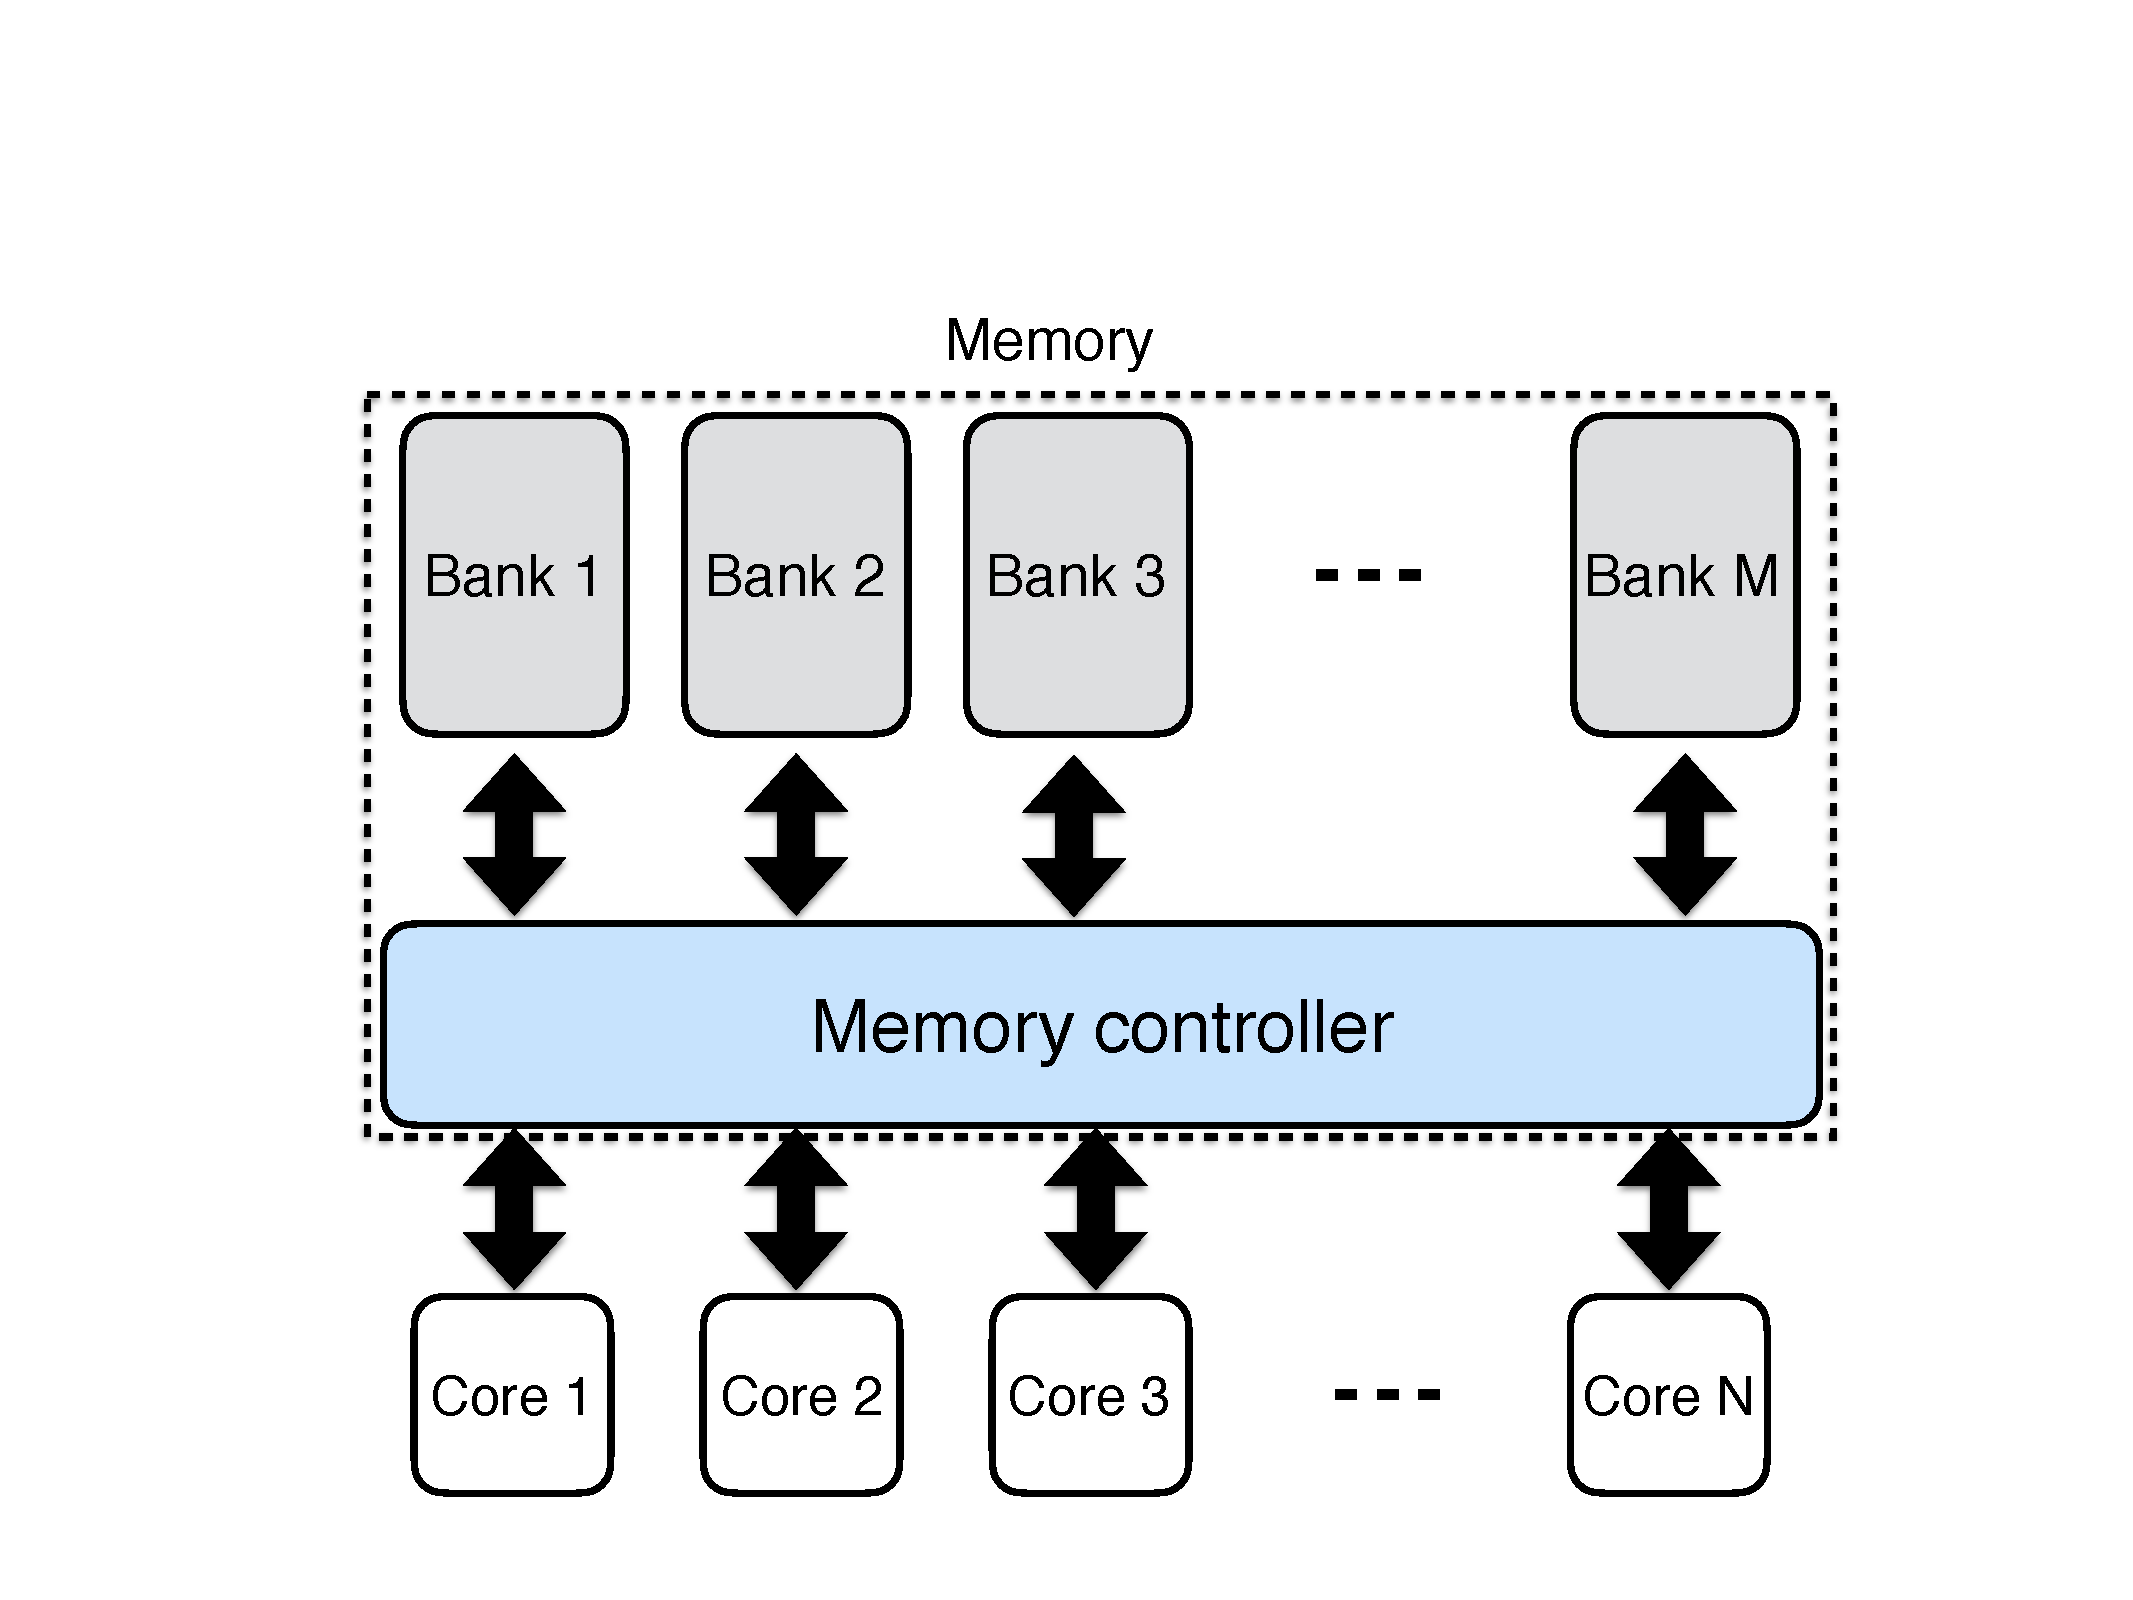
\includegraphics[width=0.85\linewidth]{figures/multicore-sys.pdf} 
\caption{Multi-core Architecture with shared memory.}
\label{fig:multicore}
\end{figure}
%%%%%%%%%%%%%%%%%%%%%%%%%%%%%%%%

 

%%%%%%%%%%%%%%%%%%%%%%%%%%%%%%%%%%%%%%%%%%%%%%
% Background and Related Work
%%%%%%%%%%%%%%%%%%%%%%%%%%%%%%%%%
\section{Background}
\label{sec:bg}

This section provides relevant background information multi-core memory architectures, and coding theory, and related work.

\subsection{Multi-core Setup and Bank Conflicts}
\label{sec:multi-core}

We consider the generic multi-core architecture illustrated in Figure~\ref{fig:multicore}, where $N$ processor cores rely on a shared memory consisting of $M$ memory banks. All the cores operate in a parallel manner and issue access requests to the shared memory in the event of last level cache misses. These access requests are received by memory controller, which then arbitrates and schedules the requests to be served by different memory banks based on the information stored on the memory banks. In particular, the memory controller maintains different queues for each of the $M$ memory banks, which hold the read and write requests corresponding to the associated bank. These queues are then sequentially served every memory cycle and the acknowledgment with data (in the case of a read requests) is sent to the processor which issued the access request. 

Assuming that the storage space of the shared memory consists of single port memory banks, i.e., it can support a single access request during a memory cycle, multiple access requests issued for content stored on the same bank cannot be served in a single memory cycle. This event is known as a \textit{bank conflict} and leads to increased access latency. The effect of these bank conflicts on the overall access latency of the shared memory becomes even more pronounced as the number of cores increases. Thus, the memory controller needs to avoid such bank conflicts while mapping the access requests from different cores to the memory banks. One straightforward solution to mitigate bank conflicts is to employ multi-port memory banks which can support multiple access requests to the same bank in a single memory cycle~\cite{patterson1997case}. However, the existing designs for multi-port memory banks suffer from increased circuit complexity and large area overhead~\cite{kapasi2003programmable}. Furthermore, in a multi-core setup with large number of cores, it is very likely for a bank to receive multiple simultaneous accesses that can exceed the number of ports present at the bank. Therefore, it's imperative to explore other solutions to the bank conflict problem beyond simply employing multi-port memory banks.

%%%%%%%%%%%%%%%%%%%%%%%%%%%%%%%%%%%%%%%%%%%%%%%%%%%%%%%%%%%%%%%%%%%%%%
%%%%%%%%%%%%%%%%%%%%%%%%%%%%%%%%%%%
%
%%%%%%%%%%%%%%%%%%%%%%%%%%%%%%%%%%%
%%%%%%%%%%%%%%%%%%%%%%%%%%%%%%%%%%%%%%%%%%%%%%%%%%%%%%%%%%%%%%%%%%%%%%
\subsection{Coding Techniques: Preliminaries}
\label{sec:coding_prelims}

Coding theory is the study of various approaches to transform available information into alternative representations with the aim of precisely controlling data redundancy, which enables reliable and efficient processing of the information. Coding has been successfully used in various fields of engineering and computer science, including communications, compression, cryptography, and data storage. The underlying transformation is referred to as a code, and its specific form depends on the application at hand. 

\subsubsection{Block Codes}
\label{sec:block-codes}
In coding theory literature, block codes are one of the most studied classes of codes. An $(n, k)$ block code transforms (encodes) $k$ message symbols belonging to a finite alphabet $\Sigma_1$ to $n$ code symbols belonging to another finite alphabet $\Sigma_2$. In many applications, these finite alphabets are finite fields which are equipped with addition and multiplication operations. The binary set $\{0, 1\}$ with modulo $2$ addition and usual multiplication is an example of a finite field. In addition, we assume that both alphabets are the same finite field $\mathbb{F}$. Under this setup, 
an $(n, k)$ block code encodes vectors in $\mathbb{F}^k$ to vectors in $\mathbb{F}^n$. The vectors in $\mathbb{F}^n$ that are obtained through the encoding process are called {\em codewords}.

The quality of a code is characterized by two parameters: 1) \textit{Rate}, which measures the amount of redundancy introduced during the transformation; and 2) \textit{Minimum distance}, which measures the maximum number of code symbols that can fail without compromising the code's ability to recover the correct message symbols. The rate of a block code is defined as 
$$
\rho = \frac{k}{n}.
$$
The minimum distance of the code $d_{\min}$ is defined as the minimum number of positions at which any two codewords differ. A block code with the minimum distance $d_{\min}$ can allow reconstruction of the original message even after the loss of any $d_{\min} - 1$ codeword symbols~\cite{MacSlo}. Ideally, one would like both the rate and the minimum distance of the underlying code to be as large as possible, however, there is a trade-off between these two parameters~\cite{MacSlo}. Most notably, the Singleton bound dictates that $d_{\min} \leq n-k+1$. Maximum distance separable (MDS) codes attain this bound with equality which makes them optimally resource efficient (as these codes achieve the highest possible rate) for a given failure tolerance. 

Reed-Solomon (RS) codes~\cite{RS1960} are the most celebrated family of MDS codes that exist for all $n$ and $k$. However, these codes typically require working with large field sizes that scale linearly with $n$. That said, we can map the arithmetic over these large fields to the operation of binary field by viewing each element of the large field as a bit vector, e.g., see \cite{shanmugam, GW16}. We will rely on vectorized RS codes in this paper. In contrast to other coding schemes that are employed in existing memory systems like SEC-DED \cite{intel}, BAMBOO \cite{kim}, and ChipKill \cite{ibm}, the RS based memory design in this paper allows for more intelligent memory controller design by improving data access.

\begin{comment}
When available, Reed Solomon codes provide an explicit MDS construction for the pair of parameters $(n,k)$. Often this comes at the expense of a large field size, but in the sequel we describe a method to map the arithmetic to binary operations on the individual bits of each byte vector \cite{shanmugam, GW16}. 
Throughout the design process, adjusting the RS parameters will allow us to achieve other points on the overhead-performance tradeoff. In contrast to other coding schemes for memory systems like SEC-DED \cite{intel}, BAMBOO \cite{kim}, and ChipKill \cite{ibm}, the proposed coding scheme allows for more intelligent memory controller design by improving data access and error correction capability.
\end{comment}

\subsubsection{Encoding Memory Banks}
\label{sec:encoding}

As mentioned above, a coding scheme is characterized by an encoding process that converts message to codewords. In the context of memory banks, we will restrict ourselves to systematic encodings, where message symbols appear as part of the codewords. In particular, we arrange the given information on some memory banks which are referred to as {\em data banks}. Then we generate {\em parity symbols} which are functions of the symbols stored in the data banks and store these parity symbols in new sets of memory banks, referred to as {\em parity banks}. Note that these additional banks, constitute the redundancy in the storage space. Furthermore, in this paper, we only consider encoding across the same row address, i.e., only the content stored on a given row address in the data banks is utilized to generate the parity symbols stored on the same row address in the parity banks.

The following example helps illustrate the key concepts and notation related to encoding memory banks to generate redundant storages space in memory systems. 

 \begin{example}
Consider the setup where information is arranged in two data banks $\mathbf{a}$ and $\mathbf{b}$. Each bank has $L$ rows, each of which can store $W$ bits. Therefore, each bank can be viewed as an $L \times W$ array. For $i \in [L] \triangleq \{1,\ldots, L\}$, let $a(i)$ and $b(i)$ denote the $i$-th row of the banks $\mathbf{a}$ and $\mathbf{b}$, respectively. Moreover, for $i \in [L]$ and $j \in [W] \triangleq \{1,\ldots, W\}$, we use $a_{i, j}$ and $b_{i, j}$ to denote the $j$-th element in the rows $a(i)$ and $b(i)$, respectively. Therefore, for $i \in [L]$,
\begin{align}
a(i) = \big(a_{i,1}, \ldots, a_{i, W}\big) \in \{0, 1\}^W,\nonumber \\
b(i) = \big(b_{i,1}, \ldots, b_{i, W}\big) \in \{0, 1\}^W. \nonumber
\end{align}
Now, given a map $f: \{0, 1\}^W \times \{0, 1\}^W \to \{0, 1\}^W$, we generate a parity bank $\mathbf{p} = f(\mathbf{a}, \mathbf{b})$ such that, for $i \in [L]$, we have
\begin{align}
p(i) = \big(p_{i, 1},\ldots, p_{i,W}\big) = f\big(a(i), b(i)\big).
\end{align}
Among many choices, if we take the function $f$ to be a bit-wise XOR, then we get $\mathbf{p} = \mathbf{a} \oplus \mathbf{b}$, i.e., for $i \in [L]$, 
\begin{align}
p(i) &= \big(p_{i, 1},\ldots, p_{i,W}\big) = a(i) \oplus b(i)\nonumber \\
&\triangleq \big(a_{i,1}\oplus b_{i,1},\ldots, a_{i,W}\oplus b_{i,W}\big). 
\end{align}
Figure~\ref{fig:example1} illustrates this coding scheme. 
%Since the parity bank is based on those rows of the data banks that are indexed by the set $[L'] \subseteq [L]$, we also use the following concise notation to represent the encoding of the parity bank. 
%$$
%\mathbf{p} = \mathbf{a}([L']) +  \mathbf{b}([L']).
%$$
%In general, we can use any subset $\mathcal{S} = \{i_1, i_2,\ldots, i_{L'}\} \subseteq [L]$ comprising $L'$ rows of data banks to generate the parity bank $\mathbf{p}$. In this case, we have
%$$
%\mathbf{p} = \mathbf{a}(\mathcal{S}) +  \mathbf{b}(\mathcal{S}),
%$$ 
%or
%$$
%p(l) = a(i_l) + b(i_l)~\text{for}~l \in [L'].
%$$
%Figure~\ref{fig:example1_case2} illustrates the case with a generic set $\mathcal{S}$.% $ = [L - L'  + 1,\ldots, L]$.
\end{example}

%------------------------------------------------------------
\begin{figure}[t!]
  \centering
  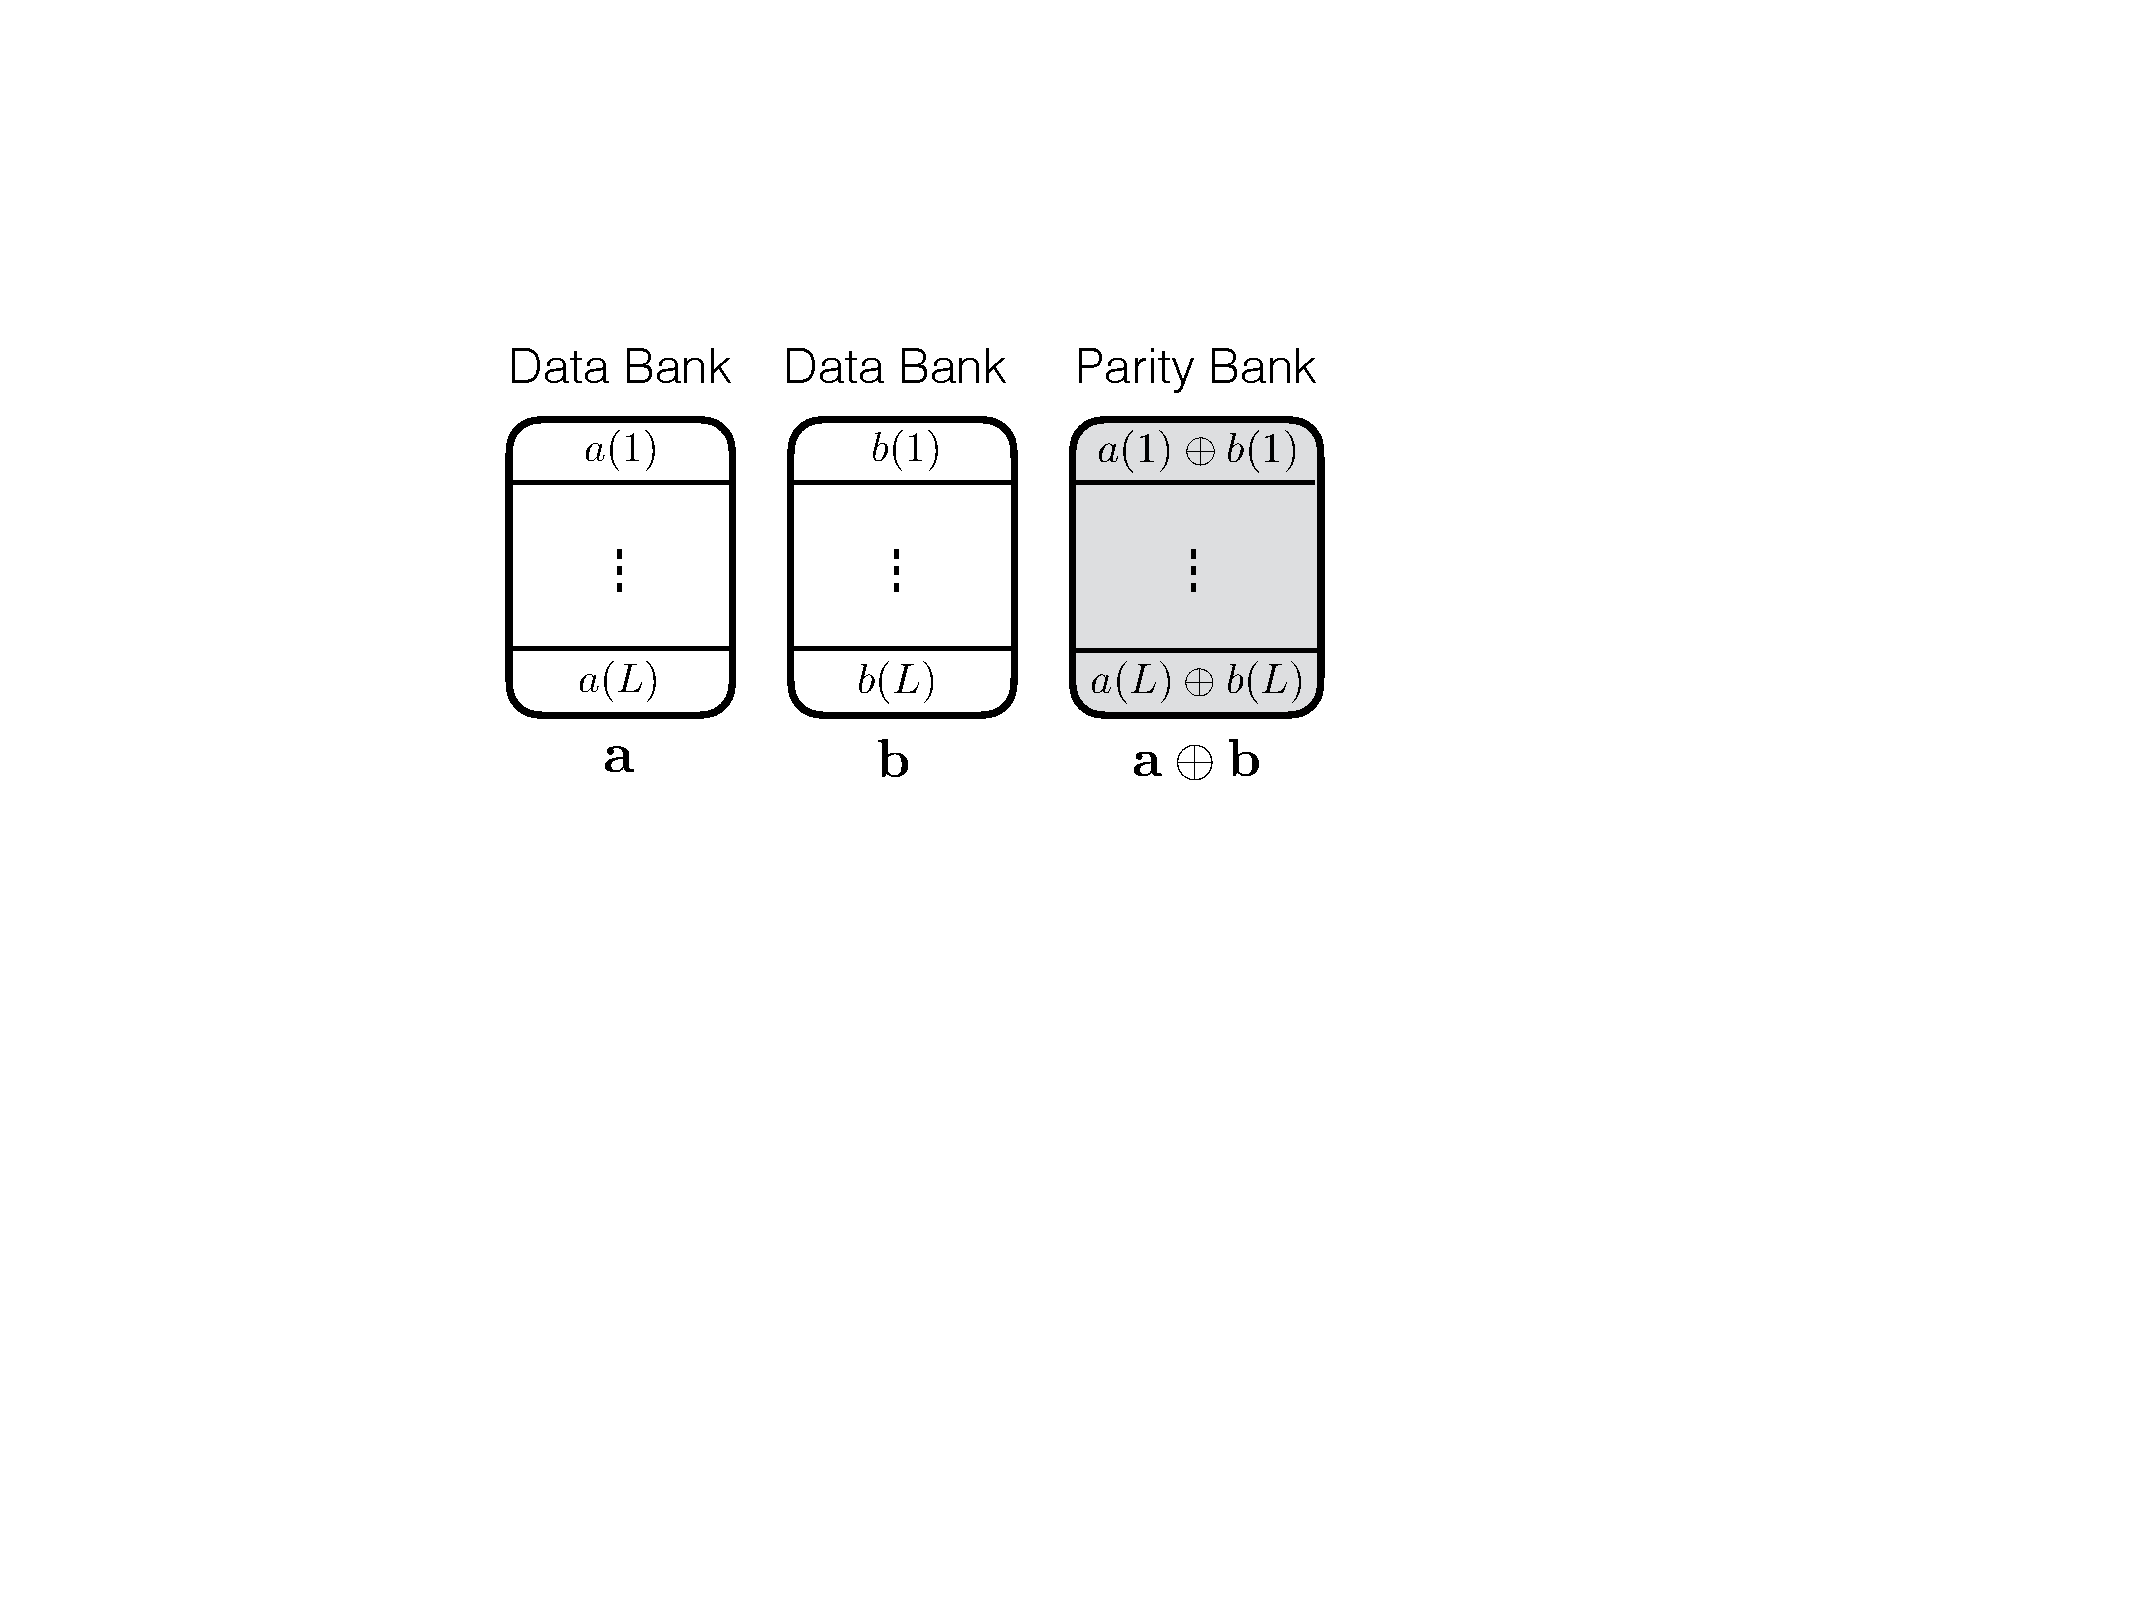
\includegraphics[width=0.65\linewidth]{figures/example-inter-bank.pdf} 
  \caption{Parity bank obtained by performing bit-wise XOR on the two data banks $\mathbf{a}$ and $\mathbf{b}$.}
  \label{fig:example1}
\end{figure}
%------------------------------------------------------------

\begin{comment}
 {\color{blue}
\begin{remark}
{\color{red} Note that we allow for the data banks and parity banks to have different sizes, i.e., $L \neq L'$. This freedom in memory design can be utilized to reduce the storage overhead of parity banks based on the underlying application. The case when the size of a parity bank is smaller than a data bank, i.e., $L' < L$, we say that the parity bank is a {\em shallow bank}. We note that it's perfectly reasonable to have the provisions for shallow banks, especially in proprietary designs of integrated memories in a system on a chip (SoC).}
\end{remark}
}
\end{comment}
%%%%%%%%%%%%%%%%%%%%%%%%%%%%%%%%%%%%%%%%%%%%%%%%%%%%%%%%%%%%%%%%%%%%%%
%%%%%%%%%%%%%%%%%%%%%%%%%%%%%%%%%%%
%
%%%%%%%%%%%%%%%%%%%%%%%%%%%%%%%%%%%
%%%%%%%%%%%%%%%%%%%%%%%%%%%%%%%%%%%%%%%%%%%%%%%%%%%%%%%%%%%%%%%%%%%%%%
\subsection{Emulating Multi-port Memories}
\label{sec:emulation}
A multi-port memory supports multiple simultaneous accesses to content stored in the same memory bank. As evident, such a memory reduces bank conflicts, where some access requests might get delayed due to a single access request accessing a particular memory bank. Therefore, multi-port memories form an essential component of a high performance multi-core setup. That said, designing true multi-port memory banks incurs large cost both in terms of circuit complexity and memory density as compared to single-port memory banks~\cite{Suzuki,WLCH14}.

This has motivated various research efforts to explore algorithm and/or system level designs to emulate the functionality of a multi-port memory using a collection of single-port memory banks, e.g., see \cite{ACP88, EMY91, RG91,CCES93, Memoir_xor, Memoir_xor_virtual} and references therein. The key idea in most of the work in this direction is to employ single port memory banks to store the content in a redundant manner. As a result, when the memory system encounters concurrent accesses leading to bank conflict in a memory bank, it uses the redundancy in the memory banks to create ways to simultaneously serve these accesses using disjoint groups of memory banks. The design of redundant storage space using single-port memory banks is typically based on two general approaches: 1) replication~\cite{ACP88}; and 2) erasure coding~\cite{RG91, Memoir_xor, Memoir_xor_virtual}. 

We briefly illustrate in Fig.~\ref{fig:emulation} how such emulations of multi-port memories work. In particular, consider a setup where we need to store $2L$ rows of data $\mathbf{a} = [a(1),\ldots, a(L)]^T$ and $\mathbf{b} = [b(1),\ldots, b(L)]^T$. We are given single-port memory banks with each bank having capacity to store $L$ rows of data. In order to simplify the exposition, we ignore the write requests for the moment. Our objective is to emulate a multi-port memory that can support $2$ simultaneous read requests to $\mathbf{a}$ and $\mathbf{b}$. Fig.~\ref{fig:emulation_r} describes a replication-based design to support $2$ simultaneous read accesses. Similarly, Fig.~\ref{fig:emulation_ec} shows how one can generate a parity bank by taking element-wise XOR of two data banks to enable $2$ simultaneous accesses. As it is evident from this example, in order to support the same number of read accesses, the replication-based scheme incurs higher storage cost as it requires more single-port memory banks to emulate a multi-port memory bank. This observation is consistent with similar trends observed in other applications, which usually provide opportunities for sophisticated coding schemes to replace replication schemes~\cite{MacSlo, Weatherspoon:2002}. However, in order to make a coding-based solution viable, especially in the context of memory systems, it is essential to employ coding schemes with low computational complexity.

It is easy to generalize the replication scheme (cf.~Fig.~\ref{fig:emulation_r}) to support $r$ simultaneous read accesses by storing $r$ copies of each data element on $r$ distinct single-port memory banks. Similarly, it is possible to employ more sophisticated coding schemes compared to the one in Fig.~\ref{fig:emulation_ec} to support multiple concurrent read accesses~\cite{batchcodes, RSDG16, WKCB17}. However, in order to translate this approach to a viable solution for a memory system, it is necessary to account for write requests as well. Note that the key challenge in employing a redundant storage space in the presence of write requests is to manage consistency across multiple copies of the data. In addition, one needs to ensure that the stale content, i.e., the content modified by a write request, is not supplied in response to a later read request. 

%--------------------------------------------------------------------
\begin{figure}[t!]
\begin{subfigure}{0.52\linewidth}
  \centering
  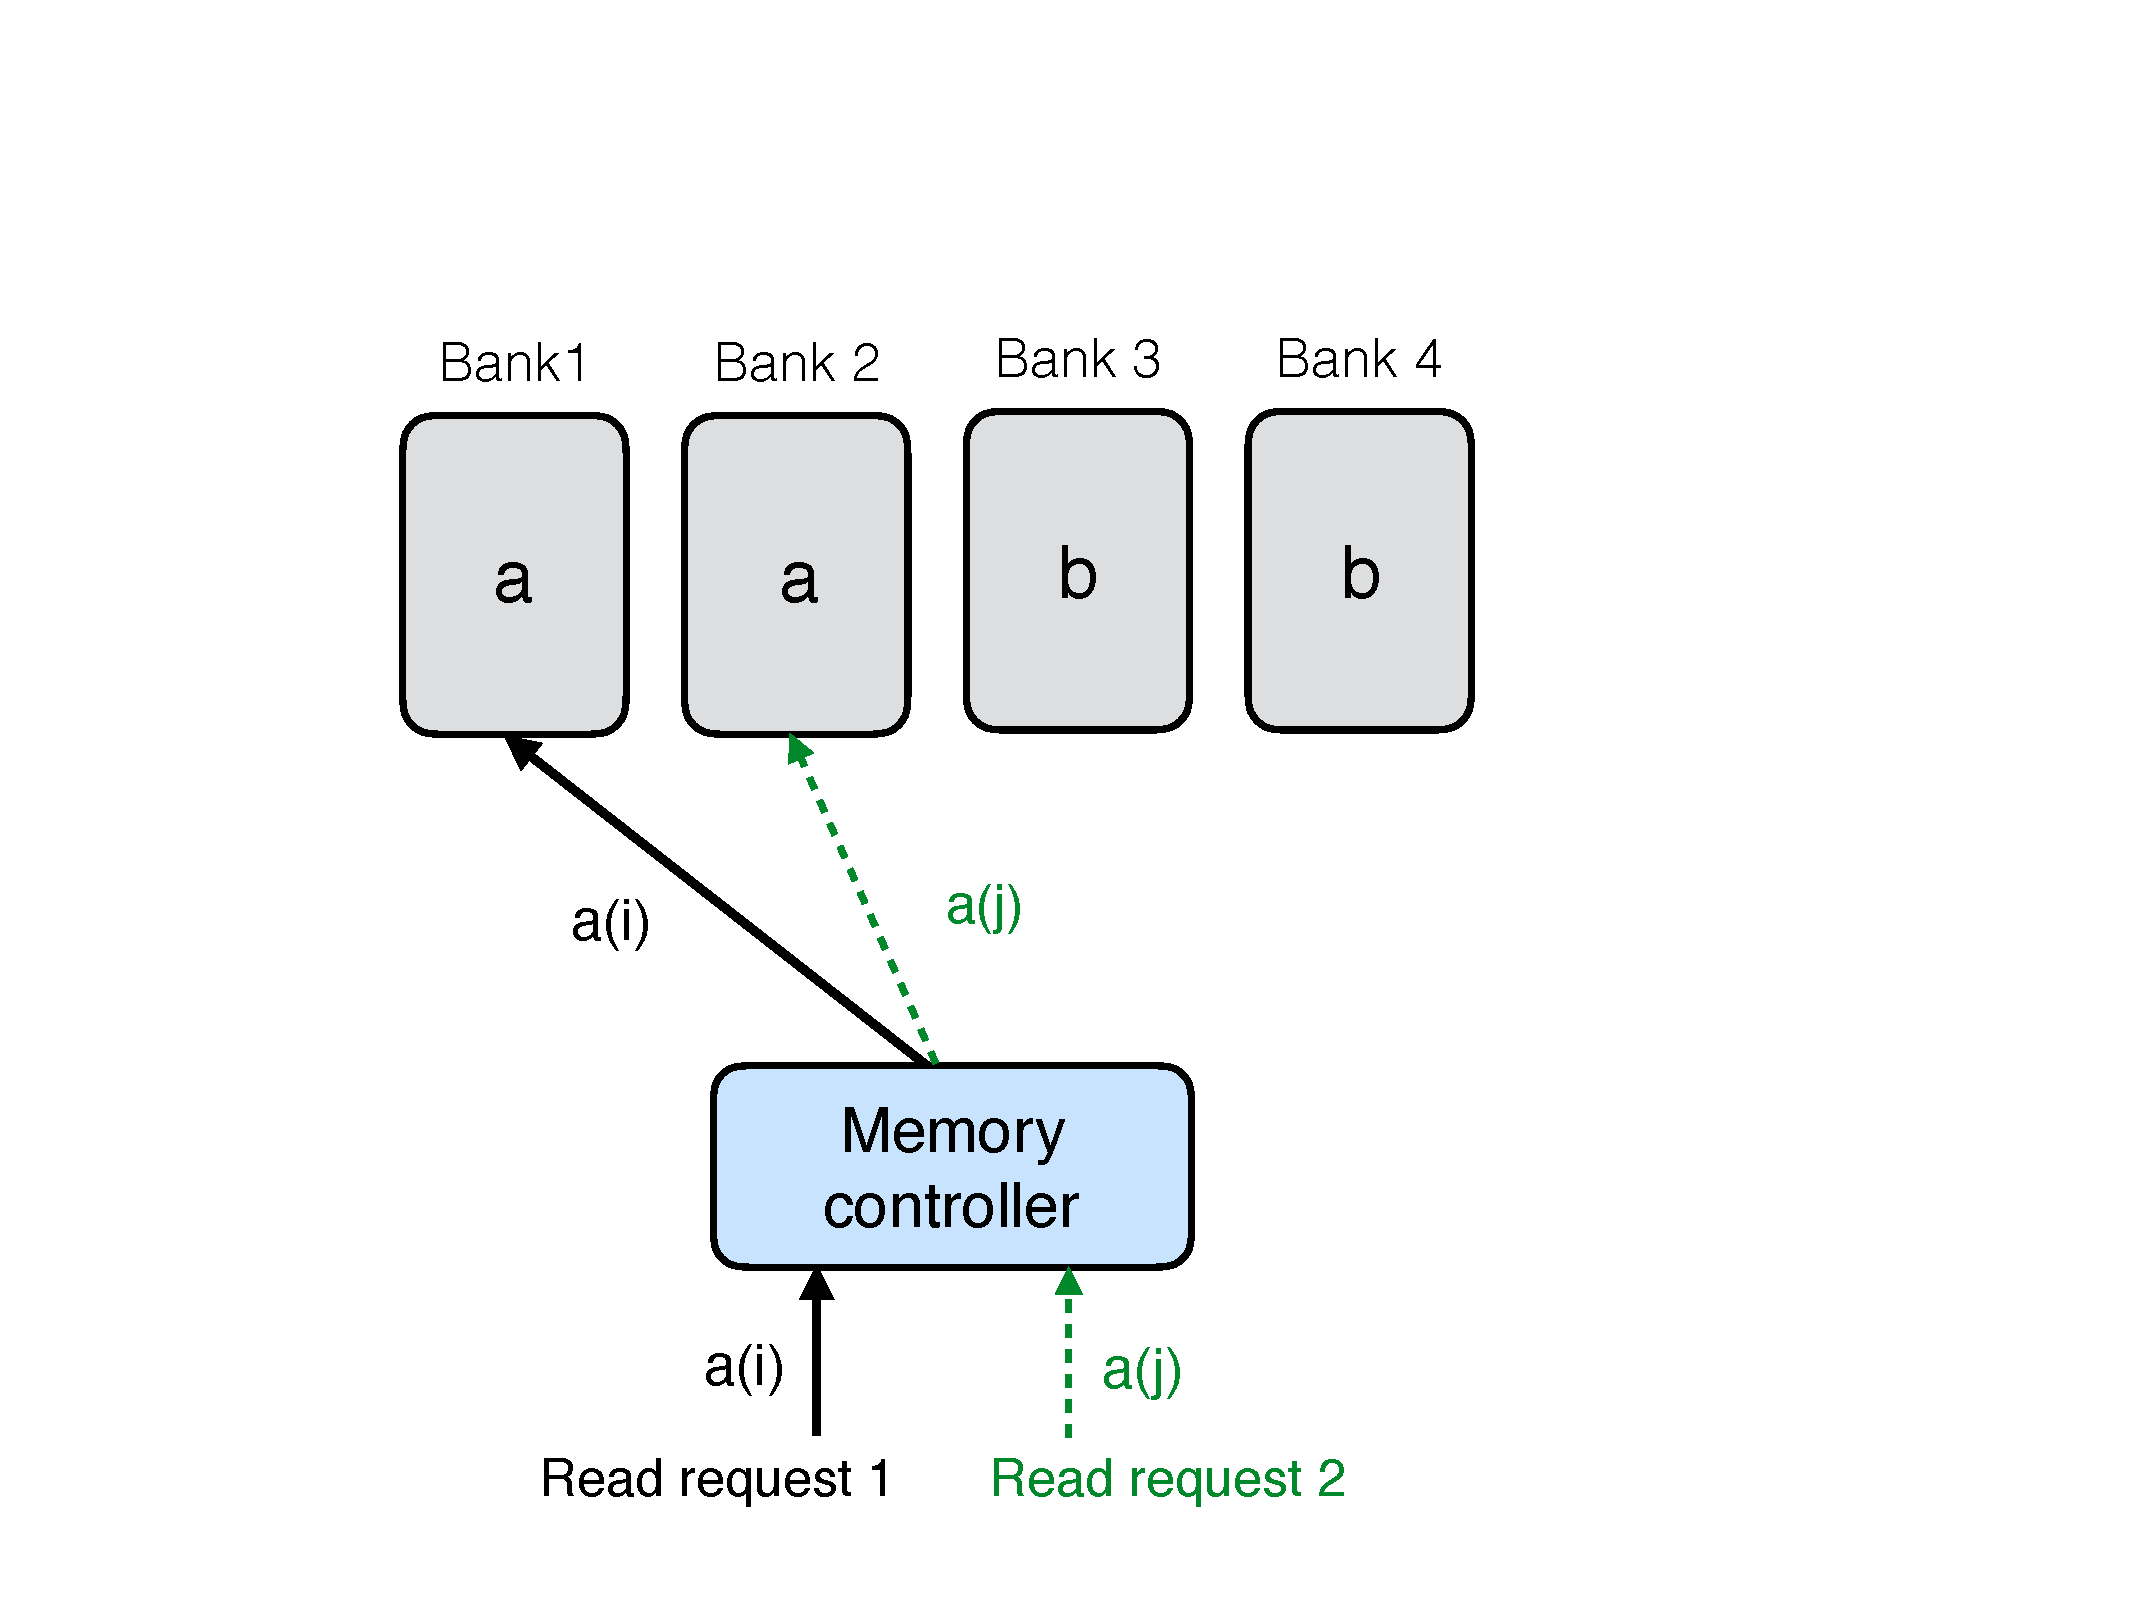
\includegraphics[height=0.92\textwidth]{figures/read-replication.pdf} 
  \caption{$2$-replication scheme.}
  \label{fig:emulation_r}
\end{subfigure}
\begin{subfigure}{0.43\linewidth}
  \centering
  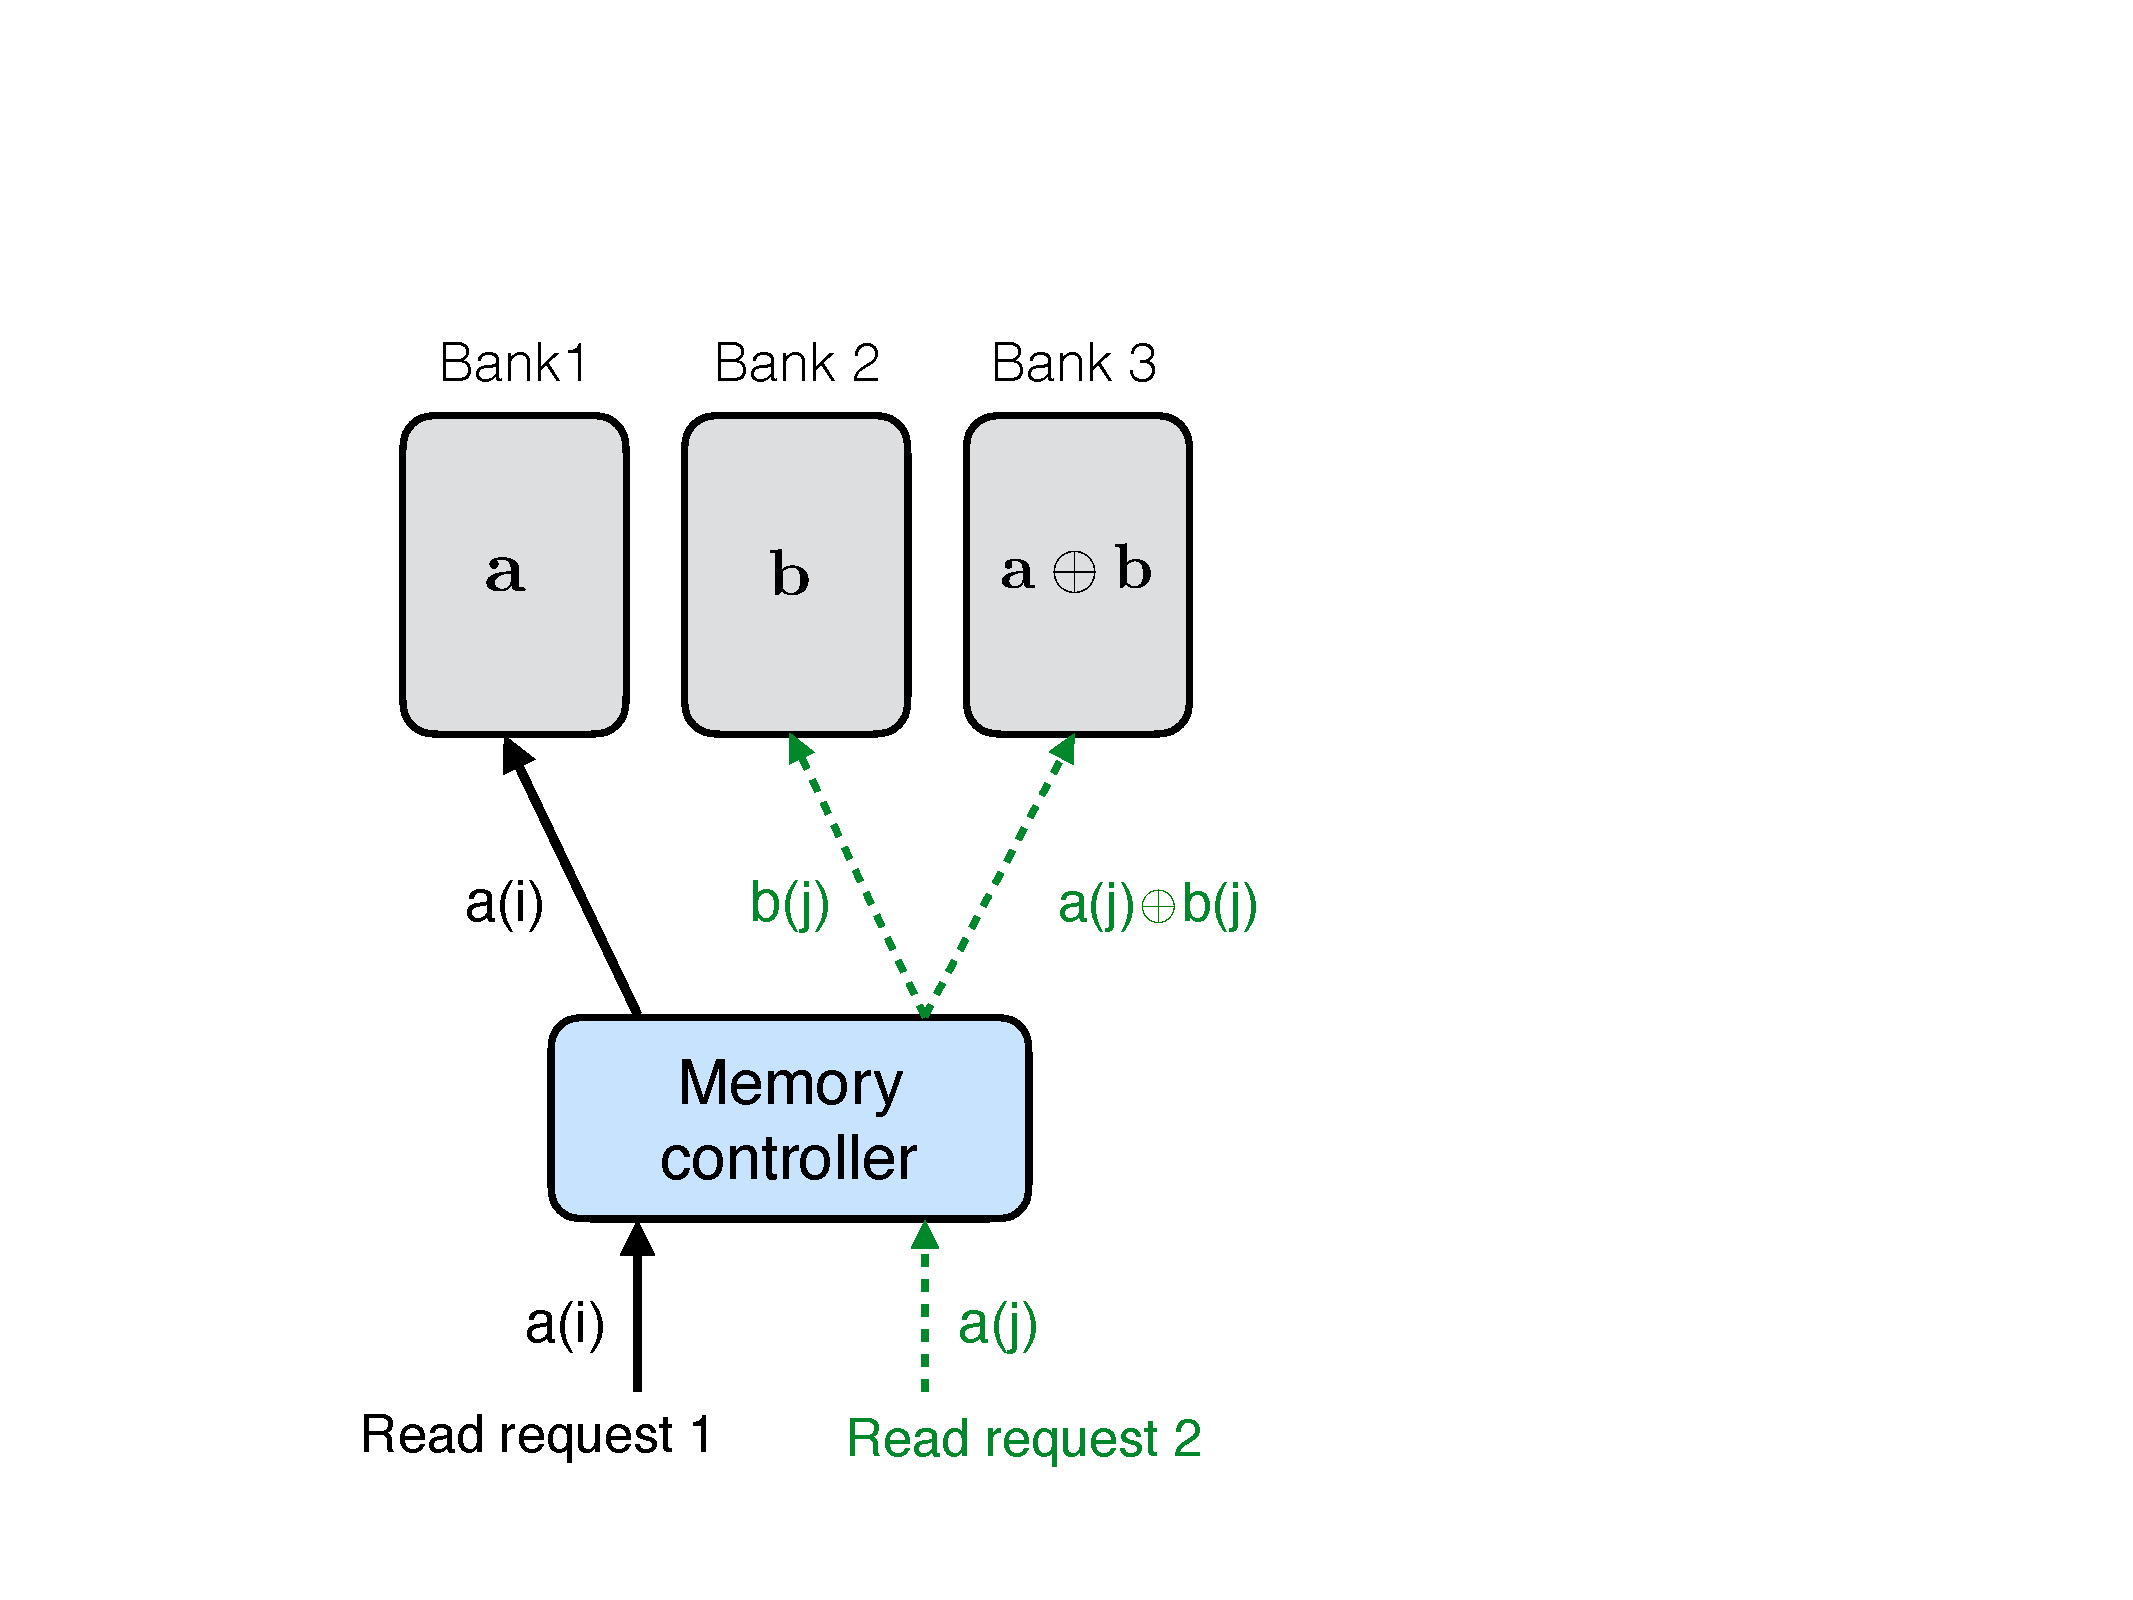
\includegraphics[height=1.1\textwidth]{figures/example-xor.pdf} 
  \caption{Bit-wise XOR.}
  \label{fig:emulation_ec}
\end{subfigure}
\caption{Supporting multiple simultaneous read accesses using single-port memory banks. Let's consider two concurrent requests for data  $\{a(i), a(j)\}$ which cause bank conflict in a single memory banks. 1)  For the replication-based design, since both $a(i)$ and $a(j)$ are stored on $2$ banks, one of those banks can be used to serve each request without causing any bank conflicts. 2) In the coded memory system, as shown in Figure~\ref{fig:emulation_ec}, we can deal with bank conflict in the following manner:  1) First request for $a(i)$ can be directly served by Bank 1, and 2) The read request for $a(j)$ can be served by downloading $b(j)$ and $a(j) + b(j)$ from Bank 2 and Bank 3, respectively.}
\label{fig:emulation}
\end{figure}
%--------------------------------------------------------------------

Towards this, Auerbach et al. demonstrate a replication-based emulation of multi-port memory using single-port memory banks~\cite{ACP88}. This emulation simultaneously supports $r$ read accesses and $w$ write accesses by storing $r\cdot(w + 1)$ copies of each data element on $r\cdot(w+1)$ distinct single-port memory banks. In order to see this, assume that these banks are partitioned in $r$ groups with each group containing $w + 1$ copies of each data element. The $r$ different groups of banks are used to serve $r$ distinct read accesses. Assuming that each group has at least one bank that stores the updated (valid) copy of each data element, we can use that bank to serve the read request from the group. In parallel, for every group, we can perform $w$ write requests on $w$ unused banks in the group. Note that this process does not cause any bank conflicts and all the write requests do get performed inside each group. 

Focusing on coding-based memory designs to support concurrent read accesses, we can modify the ideas from \cite{ACP88} to support write requests as well. We can take set of banks that support $r$ simultaneous read accesses and replicate it $(r+w)$ times~\footnote{We note that depending on the specific coding scheme, one can present a more storage-efficient design. Here, we present a universal scheme that works for any coding scheme.}. Each of these copies is referred to as a \textit{group} of banks. Now, given $r$ read requests we look for the minimum number of groups that store the most updated version of the data elements associated with these read requests and serve all the read requests. In the worst case, this would require using $r$ different groups. For the $w$ write requests, we commit these $w$ requests to $w$ different groups that are not used to serve read requests. Note that there are at least $w$ such groups. While performing a write request inside a group, we update all the memory banks of the group accordingly. 

\begin{remark} Note that the replication-based emulation described above incurs a large overall storage cost as this approach has information rate ${1}/{(r\cdot(w + 1))}$. Moreover, even though the coding-based scheme is storage-efficient in the presence of only read requests, the need to accommodate write requests makes the storage cost of this approach prohibitively large as well. Assuming that the coding scheme has information rate $\rho$, the final rate after $(r + w)$ replications is ${\rho}/{(r + w)}$. In addition to the memory banks, these designs also require additional storage space to store pointers which keep track of which memory banks store the latest versions of the data elements. In order to manage this additional storage requirement, a practical implementation must periodically synchronize every bank with the most recent version of the data.
%{\color{red}In order to keep the storage requirement for maintaining these pointers in check, we need to periodically synchronize all the banks with the most recent version of the data elements.} 
\end{remark}

In the memory architecture proposed in this paper, we completely do away with the additional replications required by the aforementioned emulation approaches to incorporate write requests. In this paper, we instead propose to handle the write requests by modifying the design of the memory controller (cf.~Section~\ref{sec:controller}). This way, we manage to preserve the storage-efficiency of a coding-based solution.

%%%%%%%%%%%%%%%%%%%%%%%%%%%%%%%%%%%%%%%%%%%%%%%%%%%%%%%%%%%%%%%%%%%%%%
%%%%%%%%%%%%%%%%%%%%%%%%%%%%%%%%%%%
%
%%%%%%%%%%%%%%%%%%%%%%%%%%%%%%%%%%%
%%%%%%%%%%%%%%%%%%%%%%%%%%%%%%%%%%%%%%%%%%%%%%%%%%%%%%%%%%%%%%%%%%%%%%

\begin{figure}[t!]
\centering
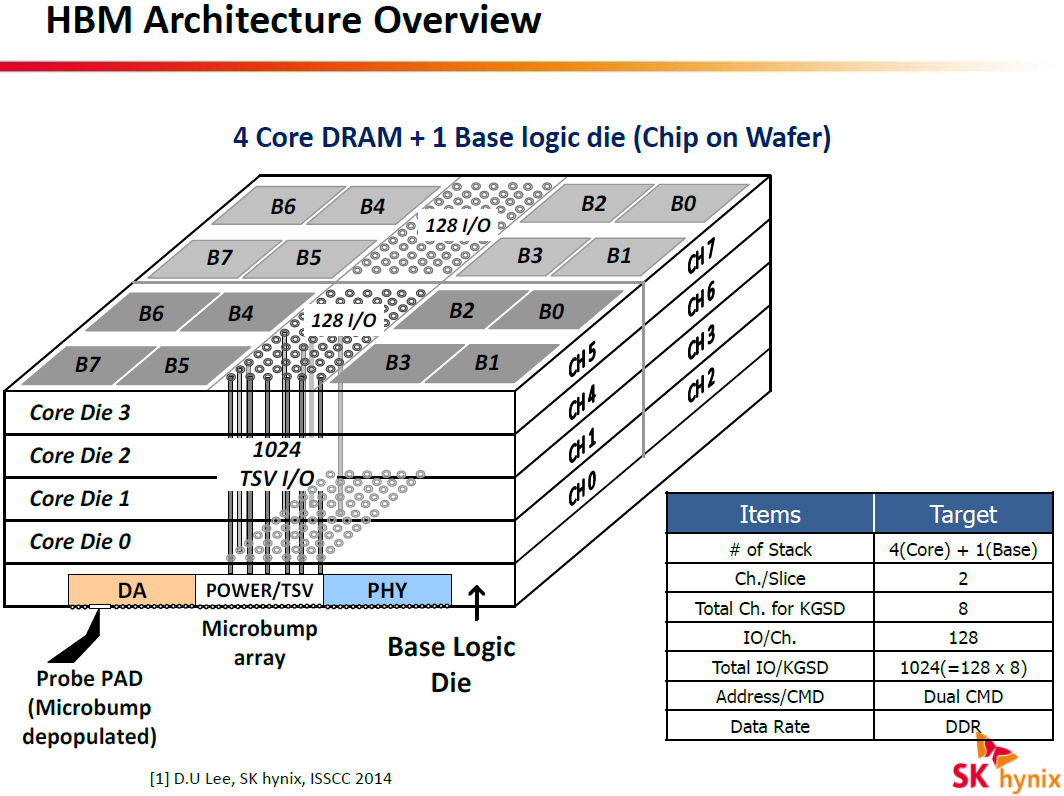
\includegraphics[width=0.99\linewidth]{figures/sk_hynix_hbm_dram_3.jpg} 
\caption{High Density Memory (HBM) architecture\protect\footnotemark. The 3D stacking of memory channels provides an orthogonal plane to pack a large amount of storage in a smaller footprint while maintaining the system's electromagnetic characteristics.}
\label{fig:hbm-arch}
\end{figure}
\footnotetext{Courtesy: \url{http://www.skhynix.com}}


\subsection{High Bandwidth Memory}
\label{sec:hbm}

High bandwidth memory (HBM) standard is defined to enable future high-performance devices such as GPUs. Figure~\ref{fig:hbm-arch} shows a stack of HBM, where it shows $4$ memory core dies vertically integrated together. Each die has $2$ channels, each one with $8$ DRAM banks ($B0$ - $B7$). This memory design enables a 3D scaling of memory, which packs more data in the same space as compared to 2D scaling, while maintaining the I/O signal integrity. The architecture also helps the computing cores to parallelize their access channels, meeting the high data access requirements while consuming less power. Here we only mention the key features of the HBM architecture that are relevant to our goal of reducing access latency using coding techniques. We refer the readers to \cite{kim2014hbm} for a detailed account of various features and specifications of the architecture. 

The key design feature of HBM that allows for parallel access to channels facilitates coded memory storage and retrieval. This enables various storage schemes where both the data and the parity symbols can be stored in the memory banks.


% There are multiple key design parameters in the HBM architecture that facilitates coded memory storage and retrieval. First, the HBM architecture enables ability to access the channels in parallel. This can allow for various storage schemes where the data and codes can be stored. Second, the HBM architecture has a provision where the memory controller can be stored closer to the memory. Additionally, it is also possible to integrate a small logic function next to each bank, which interfaces with the memory controller and performs certain preset arithmetic functions. As shown in Figure~\ref{fig:HBM}, each data bank is now capable of computing codes on the fly by accessing elements from its memory and constructing arithmetic combinations with its locally available logical block. This capability helps the code designers to structure codes which can be constructed dynamically to improve overall efficiency of the system. Local arithmetic also allows designers to draw from similar results and techniques from the field of distributed memory systems for large data servers. Finally, the HBM architecture allows for inter-bank communication, where the data from one back can directly transfer to another bank without going through the main controller. This can allow for optimal reorganization of the memory to improve the access latency. 
%This will enable a distributed memory architecture and thus, will allow for higher optimization of the flow of data and codes between the memory banks and the controller. 
%{\color{blue}Moreover, the ability to have independent channel control for clocks, timing, self refresh, and commands also enhances the capability of a coded architecture. Finally, we also note that HBM architecture provides support for bank grouping, and semi-independent row and column command interface to facilitate activate/pre-charge in parallel with read/writes.} \Ankit{Do we absolutely need the blue colored text? It sounds very vague...If we are not explicitly using these properties in our simulations..we can drop this paragraph.}

%---------------------------
\begin{figure}[t!]
\centering
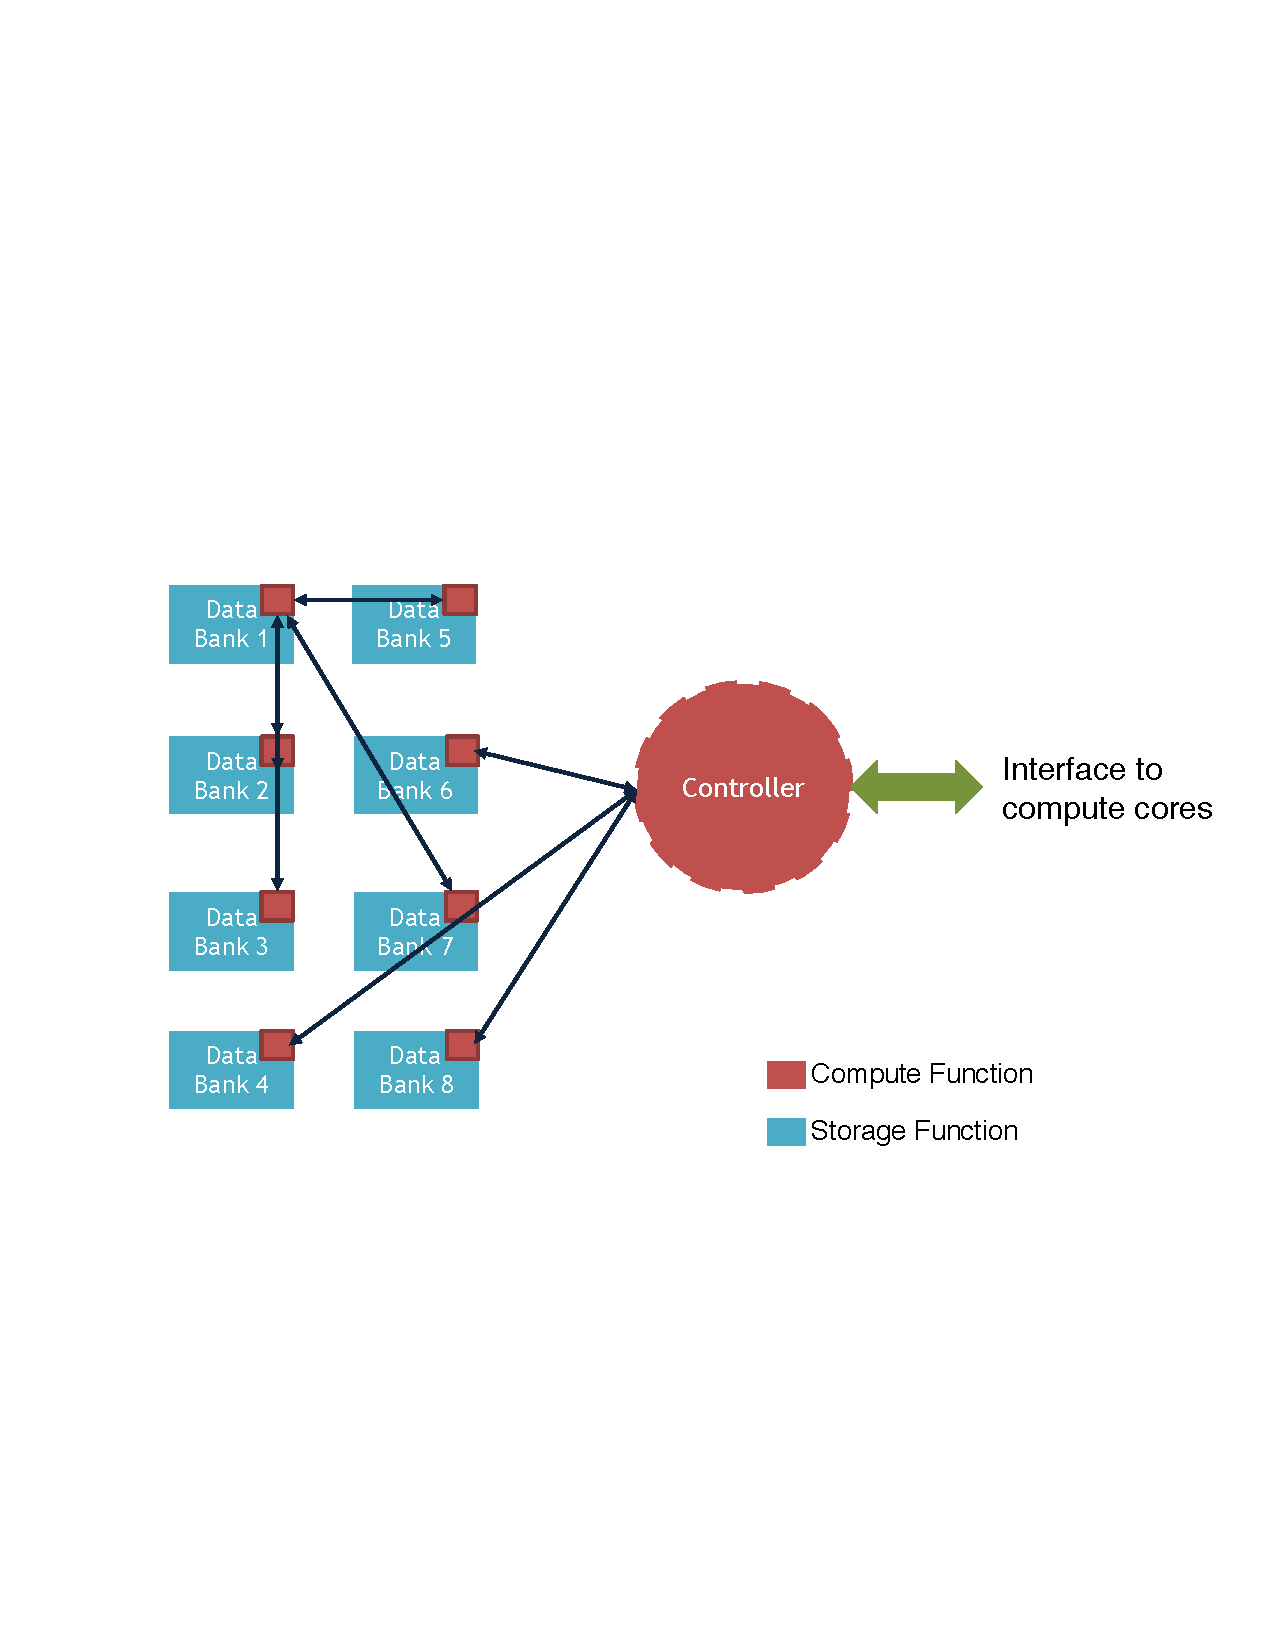
\includegraphics[width=1\linewidth]{figures/New_architecture.pdf}
\caption{Block diagram description of new memory system architectures with distributed memory controllers. This architecture includes a control logic closer to the data bank. This control logic is capable of certain fixed computation that can be exploited to reduce the access bandwidth between the bank and the main controller.%\Ethan{place compute function inside or next to storage function?}
}
\label{fig:HBM}
\end{figure}
%---------------------------

% {\color{red}
% \subsection{Hybrid memory cube}
% \label{sec:hmc}
% \Ethan{remove?}
% A hybrid memory cube (HMC) is a single package containing either four or eight DRAM die and one logic die (Figure 3), all stacked together using through-silicon via (TSV) technology. Within each cube, memory is organized vertically; portions of each memory die are combined with the corresponding portions of the other memory die in the stack. Each grouping of memory partitions is combined with a corresponding controller within the logic die, forming what is referred to as a vault.

% Key features of HMC memory organization:
% \begin{itemize}
% \item Closed-bank memory architecture
% \item Built-in memory controller for each vault
% \item Automatic refresh control over all temperatures
% \item Internal ECC data correction
% \item Advanced RAS features including data scrubbing
% \item Post-assembly repair capability
% \item In-field repair for ultimate reliability
% \item 12.5 Gb/s, 15 Gb/s, 25 Gb/s, 28 Gb/s, or 30 Gb/s SerDes I/O interface
% \item Up to four 16-lane, full-duplex serialized links
% \begin{itemize}
% \item Half-width link (8-lane) and quarter-width link (4-lane) configurations also supported
% \item Up to 320 GB/s effective bandwidth
% \end{itemize}
% \item Packet-based data/command interface
% \item Supports 16, 32, 48, 64, 80, 96, 112, 128, and 256 byte references per request
% \item Error detection (cyclic redundancy check [CRC]) for packets with automatic retry
% \item Power management supported per link
% \item Through-silicon via (TSV) technology
% \item Built-in self-test (BIST)
% \item JTAG interface (IEEE 1149.1-2001, 1149.6)
% \item I2C interface up to 1 MHz
% \item SPI master interface
% \end{itemize}
% }

\begin{remark}
We note that the Hybrid Memory Cube (HMC) architecture~\cite{HMC_slides} is somewhat similar to the HBM architecture discussed here. While our proposed approach could be used in either system, this paper focuses on HBM because it has more publicly available information and data for conducting experiments. The HMC architecture has a provision where the memory controller can be stored closer to the memory. Additionally, it is also possible to integrate a small logic function next to each bank, which interfaces with the memory controller and performs certain preset arithmetic functions. As shown in Figure~\ref{fig:HBM}, each data bank is now capable of computing parity symbols on the fly by accessing elements from its memory and constructing arithmetic combinations with its locally available logical block. This capability helps the code designers to structure codes which can be constructed dynamically to improve overall efficiency of the system. Local arithmetic also allows designers to draw from similar results and techniques from the field of distributed memory systems for large data servers. The HMC architecture also allows for inter-bank communication, where the data from one bank can directly transfer to another bank without going through the main controller. This can allow for optimal reorganization of the memory to improve the access latency. 
%This will enable a distributed memory architecture and thus, will allow for higher optimization of the flow of data and codes between the memory banks and the controller. 
\end{remark}

\newpage

%%%%%%%%%%%%%%%%%%%%%%%%%%%%%%%%%%%%%%%%%%%%%%%%%%%%%%%%%%%%%%%%%%%%%%
%%%%%%%%%%%%%%%%%%%%%%%%%%%%%%%%%%%
%
%%%%%%%%%%%%%%%%%%%%%%%%%%%%%%%%%%%
%%%%%%%%%%%%%%%%%%%%%%%%%%%%%%%%%%%%%%%%%%%%%%%%%%%%%%%%%%%%%%%%%%%%%%
\subsection{Related Work}
\label{sec:related}

\noindent {\bf Coding for distributed storage systems:~}In this paper, we employ coding techniques to store information across multiple memory banks. This is very similar to the application of coding to store data over distributed network of storage nodes in large scale storage systems~\cite{khan, dimakis, Azure12, sathiamoorthy, Hitchhiker}. However, coding for memory systems comes with stringent architectural constraints that need to be taken into account. A memory controller should not be required to perform complex computation during the accesses to the coded information. Moreover, the coding for memory systems also needs to support a significant portion of write requests during memory accesses. Therefore, even though application of coding for improved access latency has been previously explored in distributed storage systems~\cite{batchcodes, RPDV16, RSDG16, WKCB17}, achieving the same goal in the context of memory systems is a challenging problem. 

\noindent{\bf Coding for shared memory:~}In \cite{luan2017dynamic,luan2017intelligent,luan2017intelligent2}, the authors develop a coded data storage architectures which mainly applies to integrated memories in system-on-chip (SoC) subsystems. The proprietary memory design on SoC provides a lot of flexibility to design and implement a complicated coding scheme with less overhead. However, such architectures are limited to a certain subset of products and do not scale to ubiquitous DRAM memories deployed in most computing systems today. The more prevalent DRAM memories are manufactured by multiple vendors and are governed with set industry standards and protocols. Interoperability with commercial devices (and conformity to standards) requires a new design for coded data storage, one which can be implemented by enhancing the memory controller and enables the benefits of a coded architecture. The coding schemes described in \cite{luan2017dynamic,luan2017intelligent,luan2017intelligent2} are suboptimal for the standard memory systems including DRAM and HBM as their specific architectures (cf.~Section~\ref{sec:hbm}) provide the opportunities for further optimization.

In \cite{RG91, Memoir_xor, Memoir_xor_virtual}, the authors also explore coding theoretic techniques in memory systems in order to emulate multi-port memory using single-port memory banks. However, we note that the overall solution proposed in this paper significantly differs from this prior work in both the employed code design and the accompanied memory controller architecture. 

As mentioned earlier, there have been multiple efforts in realizing multi-port memory functionality using various circuit designs (e.g., see \cite{EMY91} and references therein). In this paper we focus on a coding theoretic approach to explore an orthogonal design space. We believe that the previously studied techniques, e.g. pipelined, time-sharing access~\cite{EMY91}, may very well be combined with our coding theoretic framework in order to obtain a more comprehensive solution for high performance memory systems.

%%%%%%%%%%%%%%%%%%%%%%%%%%%%%%%%%%%%%%%%%%%%%%
% Code design
%%%%%%%%%%%%%%%%%%%%%%%%%%%%%%%%%
%  


\begin{comment}
%%%%%%%%%%%%%%%%%%%%%%%%%%%%%%%%%%%
\begin{figure*}[t!]
\begin{subfigure}[htb]{0.42\linewidth}
  \centering
  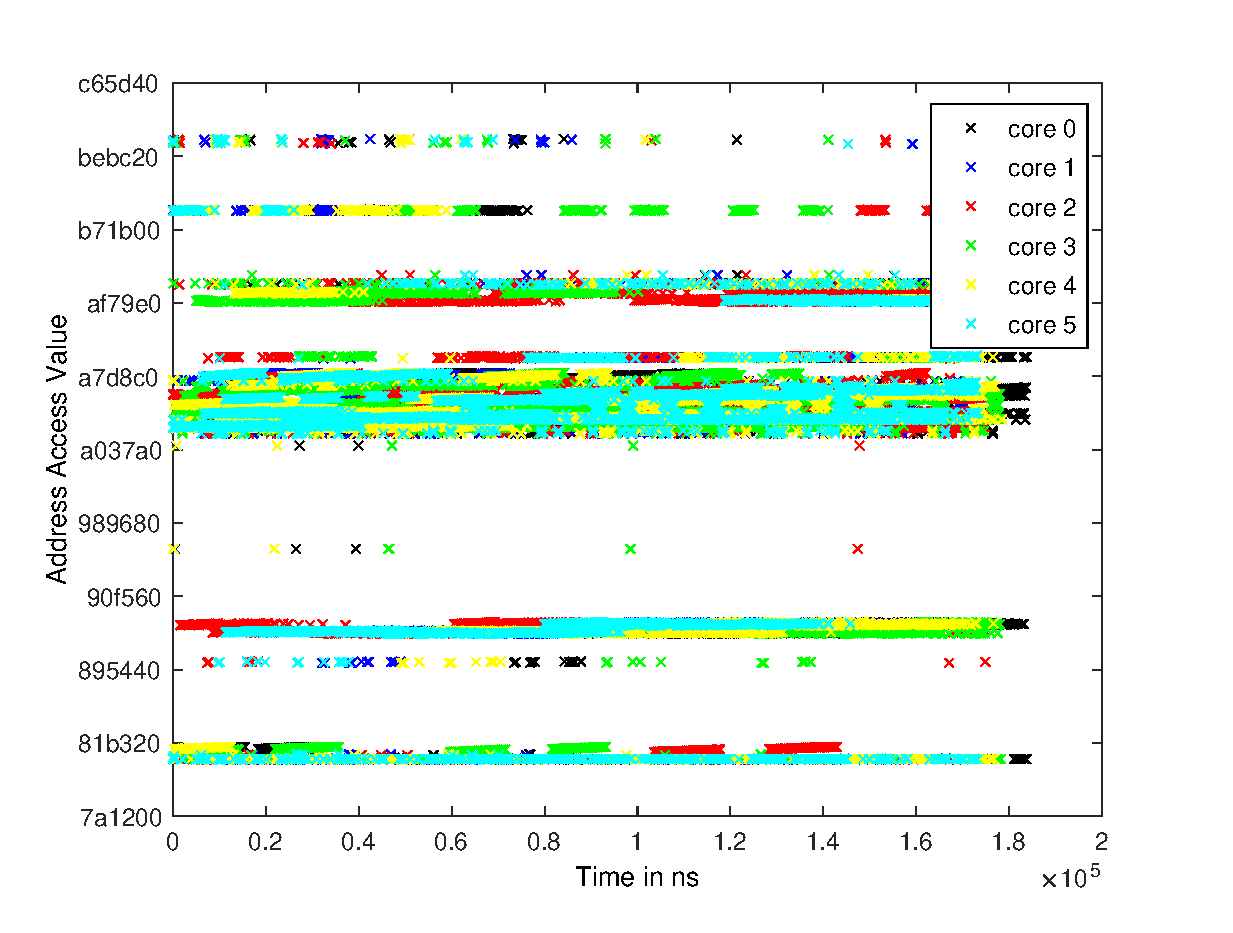
\includegraphics[height=\textwidth]{figures/add-access-soc1.eps} 
  \caption{This is a address access trace taken from a real multi-core SoC system that shows the performance of the data memory access pattern while it is executing commands. Access patterns are bulky in general.}
  \label{fig:dynamic_coding1}
\end{subfigure}
\hspace*{\fill}
\begin{subfigure}[htb]{0.42\linewidth}
  \centering
  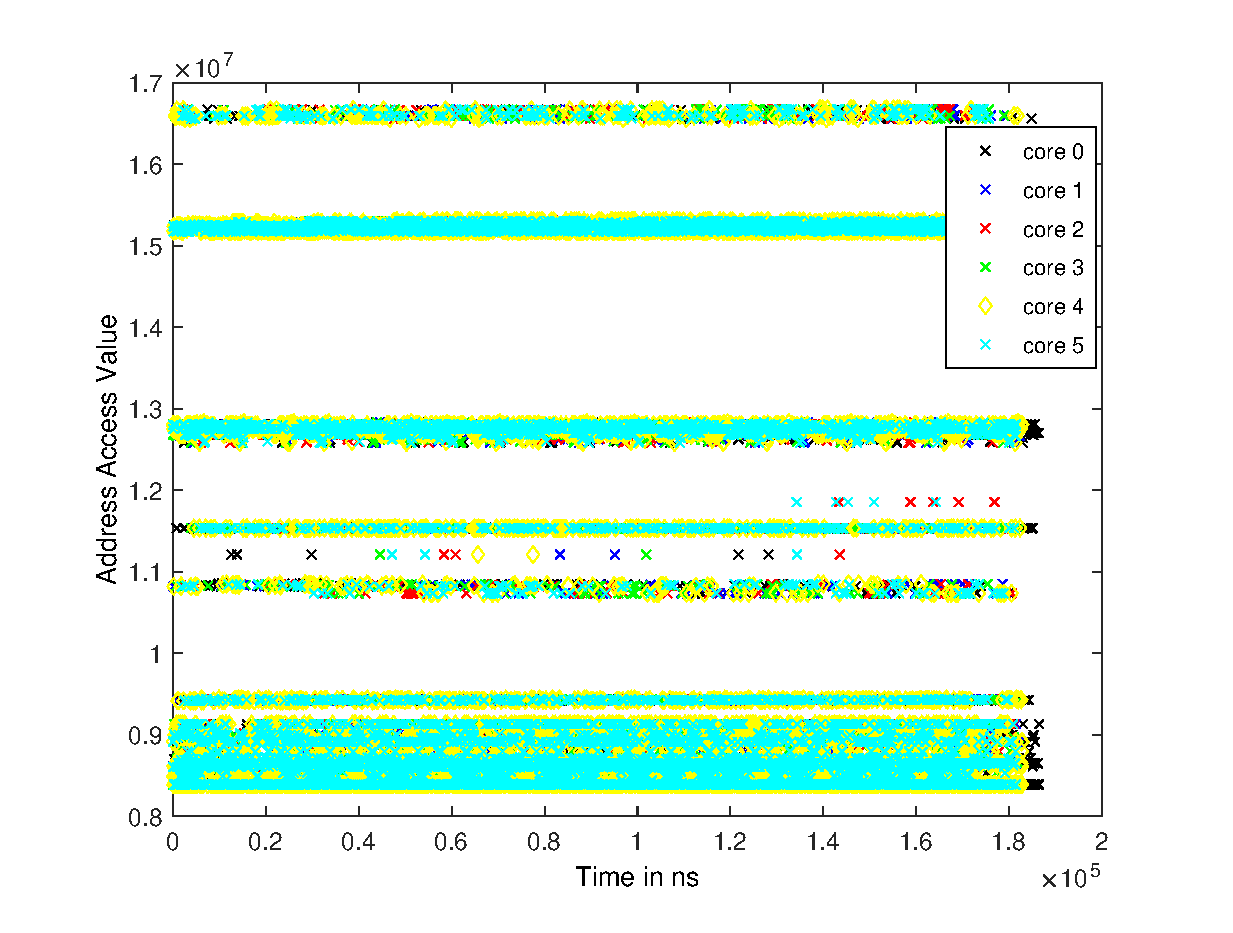
\includegraphics[height=\textwidth]{figures/add-access-soc2.eps} 
  \caption{This is an accesss pattern from another SoC system showing a multi-core access. The accesses here is more concentrated on smaller memory regions where the proposed scheme in this paper can help spread out the access resulting in higher latency. }
  \label{fig:dynamic_coding2}
\end{subfigure}
\caption{Illustration of the locality in memory access patterns using two real-life traces.}
\label{fig:dynamic_coding}
\end{figure*}
%%%%%%%%%%%%%%%%%%%%%%%%%%%%%%%%%%%%%%


\subsubsection{Dynamic coding}
\Ethan{Remove entire subsection?}
The contention in memory accesses from various cores occurs mostly when the access are to shared memory, especially when they are localized to certain memory regions. We explore the locality of the memory access over a period of time to reduce the memory overhead for storing the codes. In a multi-core system, when various cores try to work from a shared memory location, they tend to generate accesses to a localized region of memory. This motivates the idea of coding the localized region during the period of heavy access, and dynamically changing the region whenever there is change in the locality of memory accesses.

Figure \ref{fig:dynamic_coding1} shows the access pattern of a wireless SoC cores $0$ to $6$. The $y$-axis of the figure shows the address accessed by the first set of wireless SoC cores over a period of time. The $x$-axis denotes the time in nanoseconds. This plot shows that most of the access from various cores are limited to the memory range from \texttt{0x007a1200} to \texttt{0x00c65d40} (lower and higher range on the $y$-axis). It also suggests that most (about 60\%) of the accesses belong to the memory region of \texttt{0x00a037a0} to \texttt{0x00b71b00}. We make similar observation from Figure \ref{fig:dynamic_coding2} for another set of traces with highly concentrated, spottier access patterns. Here again, all of the access for a duration of approximately 0.2 ms is in the address range of \texttt{0x007a1200} to \texttt{0x01036640}.

From the above observations, we demonstrate the idea of coding the highly accessed portion of the memory. This scheme benefits from a huge reduction of the memory overhead with coding. The reduction the memory overhead can be used to reduce the complexity of the decoder by using simple coding functions (e.g. XOR) and for densely coding (e.g. repeatedly coding a single element using 2 elements). 
The scheme of dynamic coding requires that the currently coded region changes when the access pattern changes. That is, the localized memory area that is most heavily accessed can change, and it will require the system to recode the new localized access region. We assume that the working area of a program changes with change in the input parameters to the program. It can be easily observed from the above figures that the working area or the localized area is constant for at least $0.2$ ms\Ankit{Is $0.2$ ms long enough?}. This suggests that the switching of the coded region is not very frequent. During these periods of coding switches, it is also guaranteed that the number of accesses served from the memory is at worst equal to the number of banks available. In other words, coding the memory has no performance degradation compared to non-coding during these times. 

The system also needs to maintain an algorithm to observe the access pattern of the cores, and make a decision when it is time to code a new memory region. To do this, the memory controller tracks the most accessible region during a time period and makes a decision to slide/shift the coded region. This shift in the coded region requires the update of the parity bank for the new region. This process is carried out in conjunction with the ongoing access to the newly coded region. Therefore, this operation only requires writes to the parity banks, since we can use the current reads from the coded region to access the data that is to be coded. In addition, reads are also scheduled in the idle periods, when there is no read or write request to the bank/banks.


Dynamic coding requires the system to divide the memory into subregions and to keep track of accesses in these sub-regions. Once the number of accesses to a sub-region reaches a given threshold, it must then make this region the currently coded area. We propose this mechanism based on window concept. The system maintains a tuple of sub-regions such as [Starting Address, Length]. Each sub-region is thus given a starting address and length. Any access to a particular sub-region is considered as a hit. The system has a hit counter associated with each of the sub-region which is incremented for each hit. The system makes a decision of coding a particular sub-region based on its counter value. The number of coded sub-regions at a particular time is based on the sub-region size and the code storage size. The eviction of a coded region follows the LRU policy similar to cache.


%%%%%%%%%%%%%%%%%%%%%%%%%%%%%%%%%%%
\begin{figure*}[htb] \centering
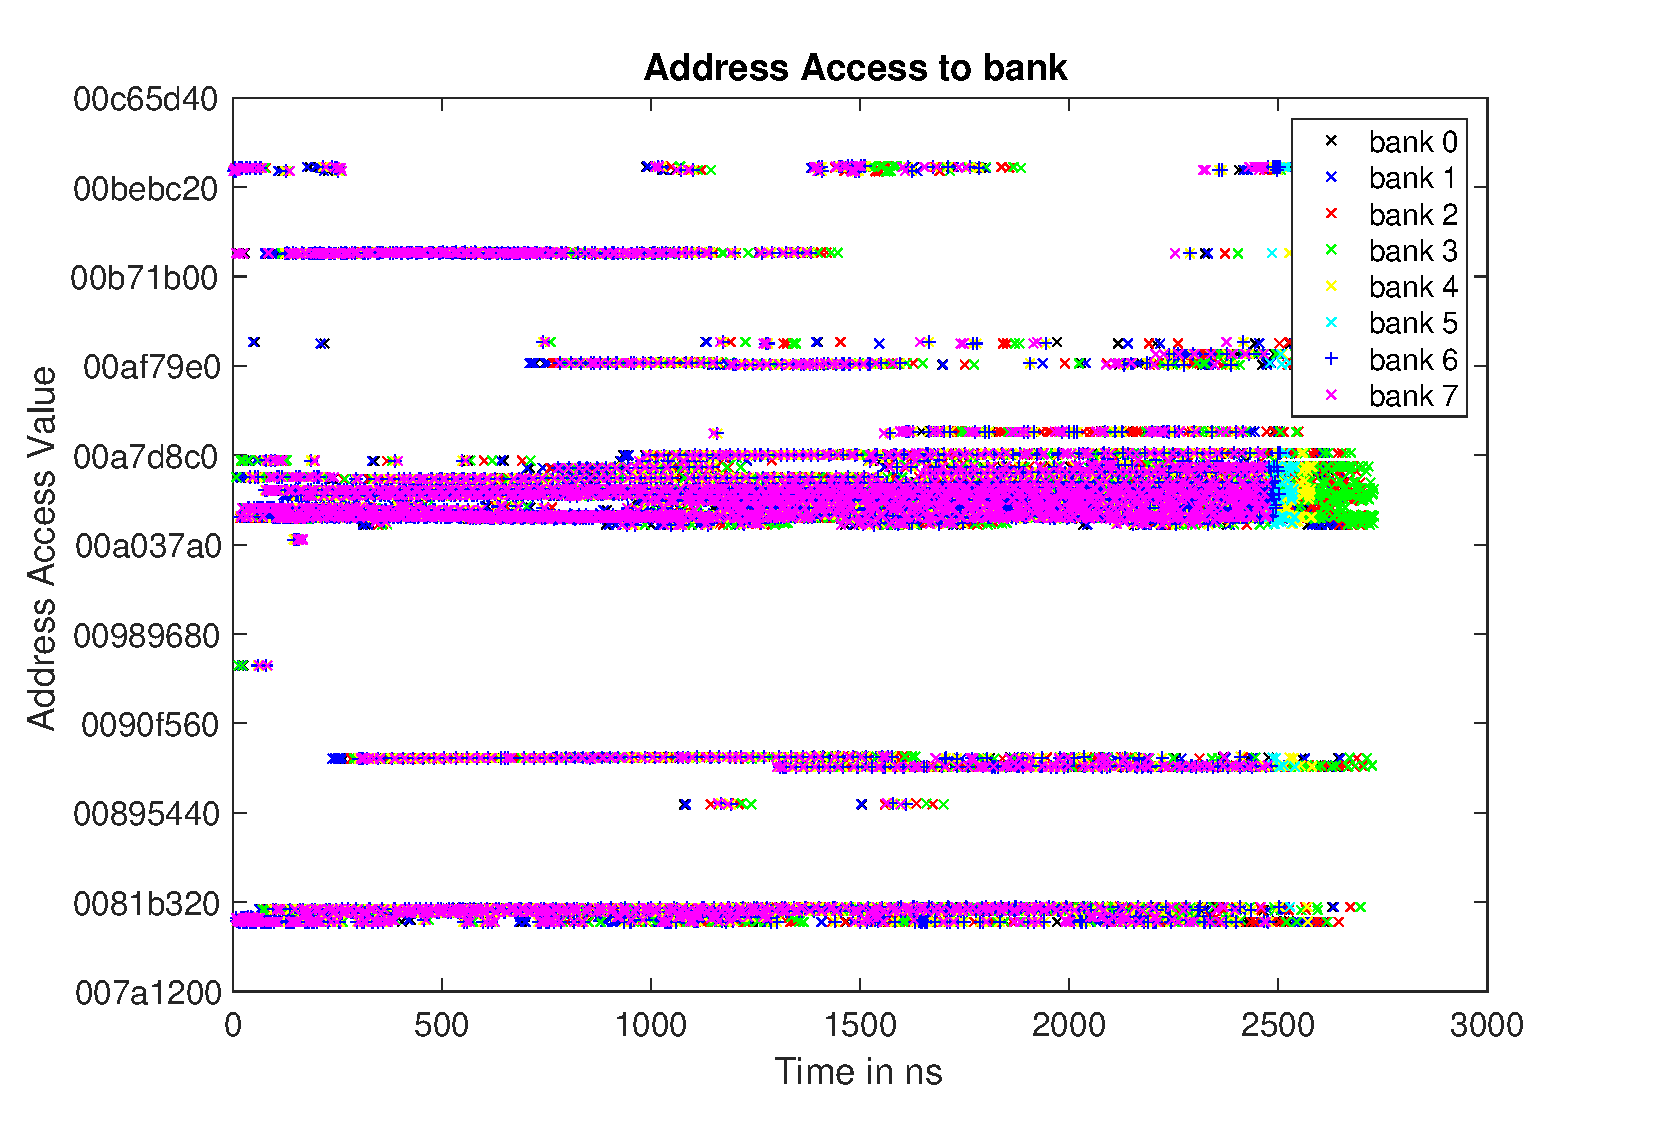
\includegraphics[width=0.48\linewidth]{figures/prefetch1.eps} 
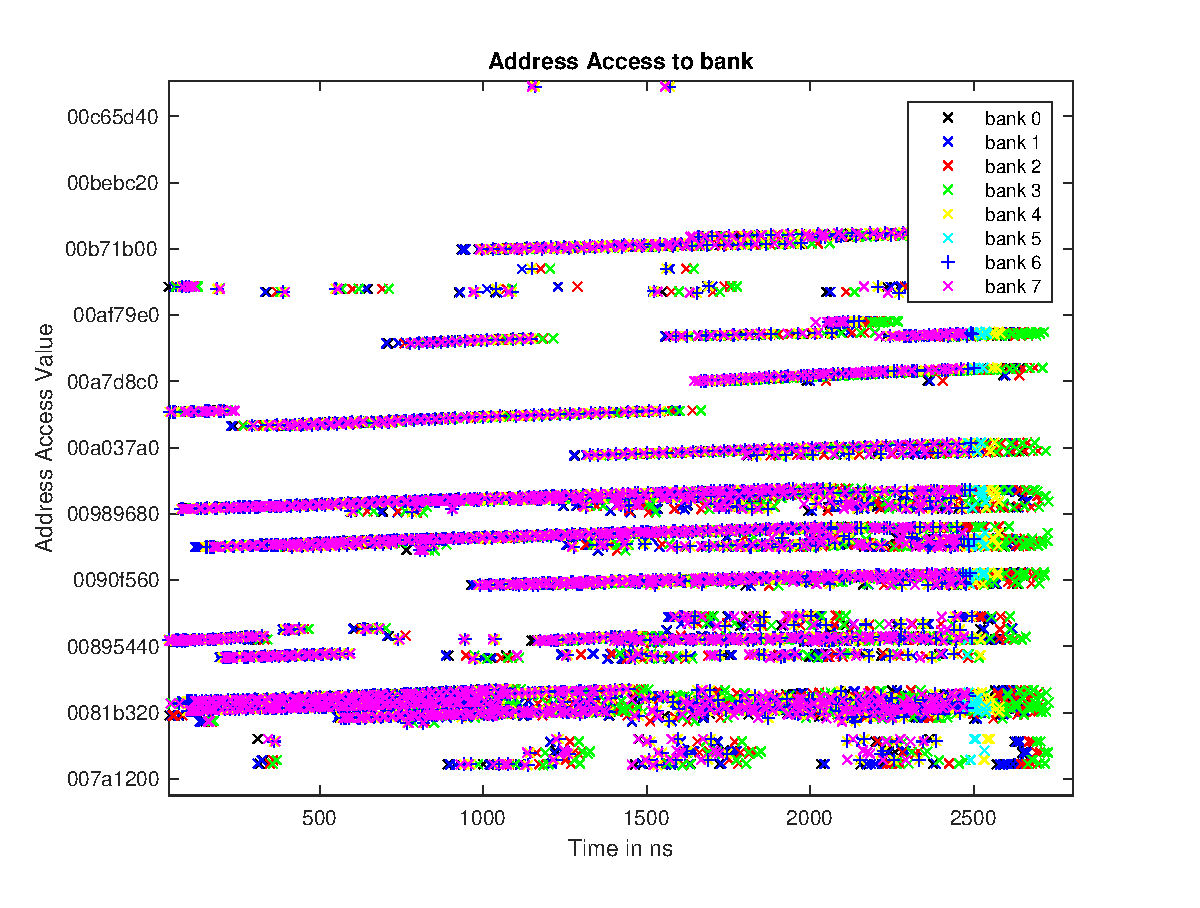
\includegraphics[width=0.48\linewidth]{figures/prefetch2.eps} 
\caption{memory accesses to a bank with respect to time}
\label{fig:prefetch1}
\end{figure*}
%%%%%%%%%%%%%%%%%%%%%%%%%%%%%%%%%%%

\subsubsection{Prefetching codes}
\Ethan{Remove entire subsection?}
The technique of dynamic coding reduces the memory overhead by exploiting the localized nature of memory accesses from the cores. In this subsection, we explore prefetching the coded data to reduce the access overhead and contention caused for fetching the codes. This is done by using the gaps in the memory access to any bank and using these gaps to prefetch the code/data for a future memory access. During a program, there are access cycles when certain banks do not have any access scheduled for a read/write. We propose the prefetching technique where we look forward in the queue and anticipate a prefetch for the data/code for that bank. We explore the implementation of a memory prefetching unit, similar to an instruction or cache prefetching unit. This unit can detect linear access patterns to regions in memory.  For example, if a string of memory accesses are issued in sequential byte sized order, then the prefetching unit will predict the next access to be in byte increments. The memory prefetching works by fetching a predicted address from the parity bank during accesses that the parity bank is idle. When future memory accesses are issued, they are first checked with the prefetched data to see if they can be used to decode any subsequent accesses memory accesses. If so, the memory access is obtained from the current accesses and prefetched data. 

For example, say the prefetcher sees 2 consecutive memory requests in a row. It then predicts that the next two accesses, locations $a_0$ and $b_0$, are likely to be accessed in the near future. It reads $a_0 + b_0$ from the parity bank for future use. Next, access to location $a_0$ and $b_0$ are issued to the memory. Now, instead of reading both $a_0$ and $b_0$, only a single location has to be read from in memory, while the other location can be obtained from the prefetched data. This allows for an additional access to be issued from the now free memory bank.  In these cases, it is possible to obtain up to two additional memory accesses in a given cycle, one from the prefetched data and one from the parity bank.

Implementation of a memory prefetch should only require overhead for space and the associated logic to implement it. Since memory accesses are often stalled due to bank conflicts, checking pending accesses to the prefetched data should require no additional time overhead. As memory accesses wait to be issued in the bank queues, they can simultaneously be checked with the prefetched data. Thus, no extra latency is anticipated by the addition of a memory prefetching unit.

Figure~\ref{fig:prefetch1} shows two plots of memory accesses to a bank with respect to time. The left figure shows the accesses to the memory bank by various cores. The right side figure shows a zoomed view of the accesses in the dense access region. This figure suggests the linearity of accesses. The system can look ahead in the queue to detect the consecutive address request for a memory bank and schedule a prefetch of the associated code. In Figure~\ref{fig:prefetch2}, we simulate the prefetching of the code by using a window of length $100$. That is, we look ahead to $100$ request in the queue and find out the occurrence of consecutive address in the window. The plot suggest high occurrence of the consecutive addresses in the bank which can be served by prefetching the codes. 
\end{comment}

%%%%%%%%%%%%%%%%%%%%%%%%%%%%%%%%%%%%%%%%%%%%%%
% Coding Architecture for HBM
%%%%%%%%%%%%%%%%%%%%%%%%%%%%%%%%%
\begin{figure*}[t!] \centering
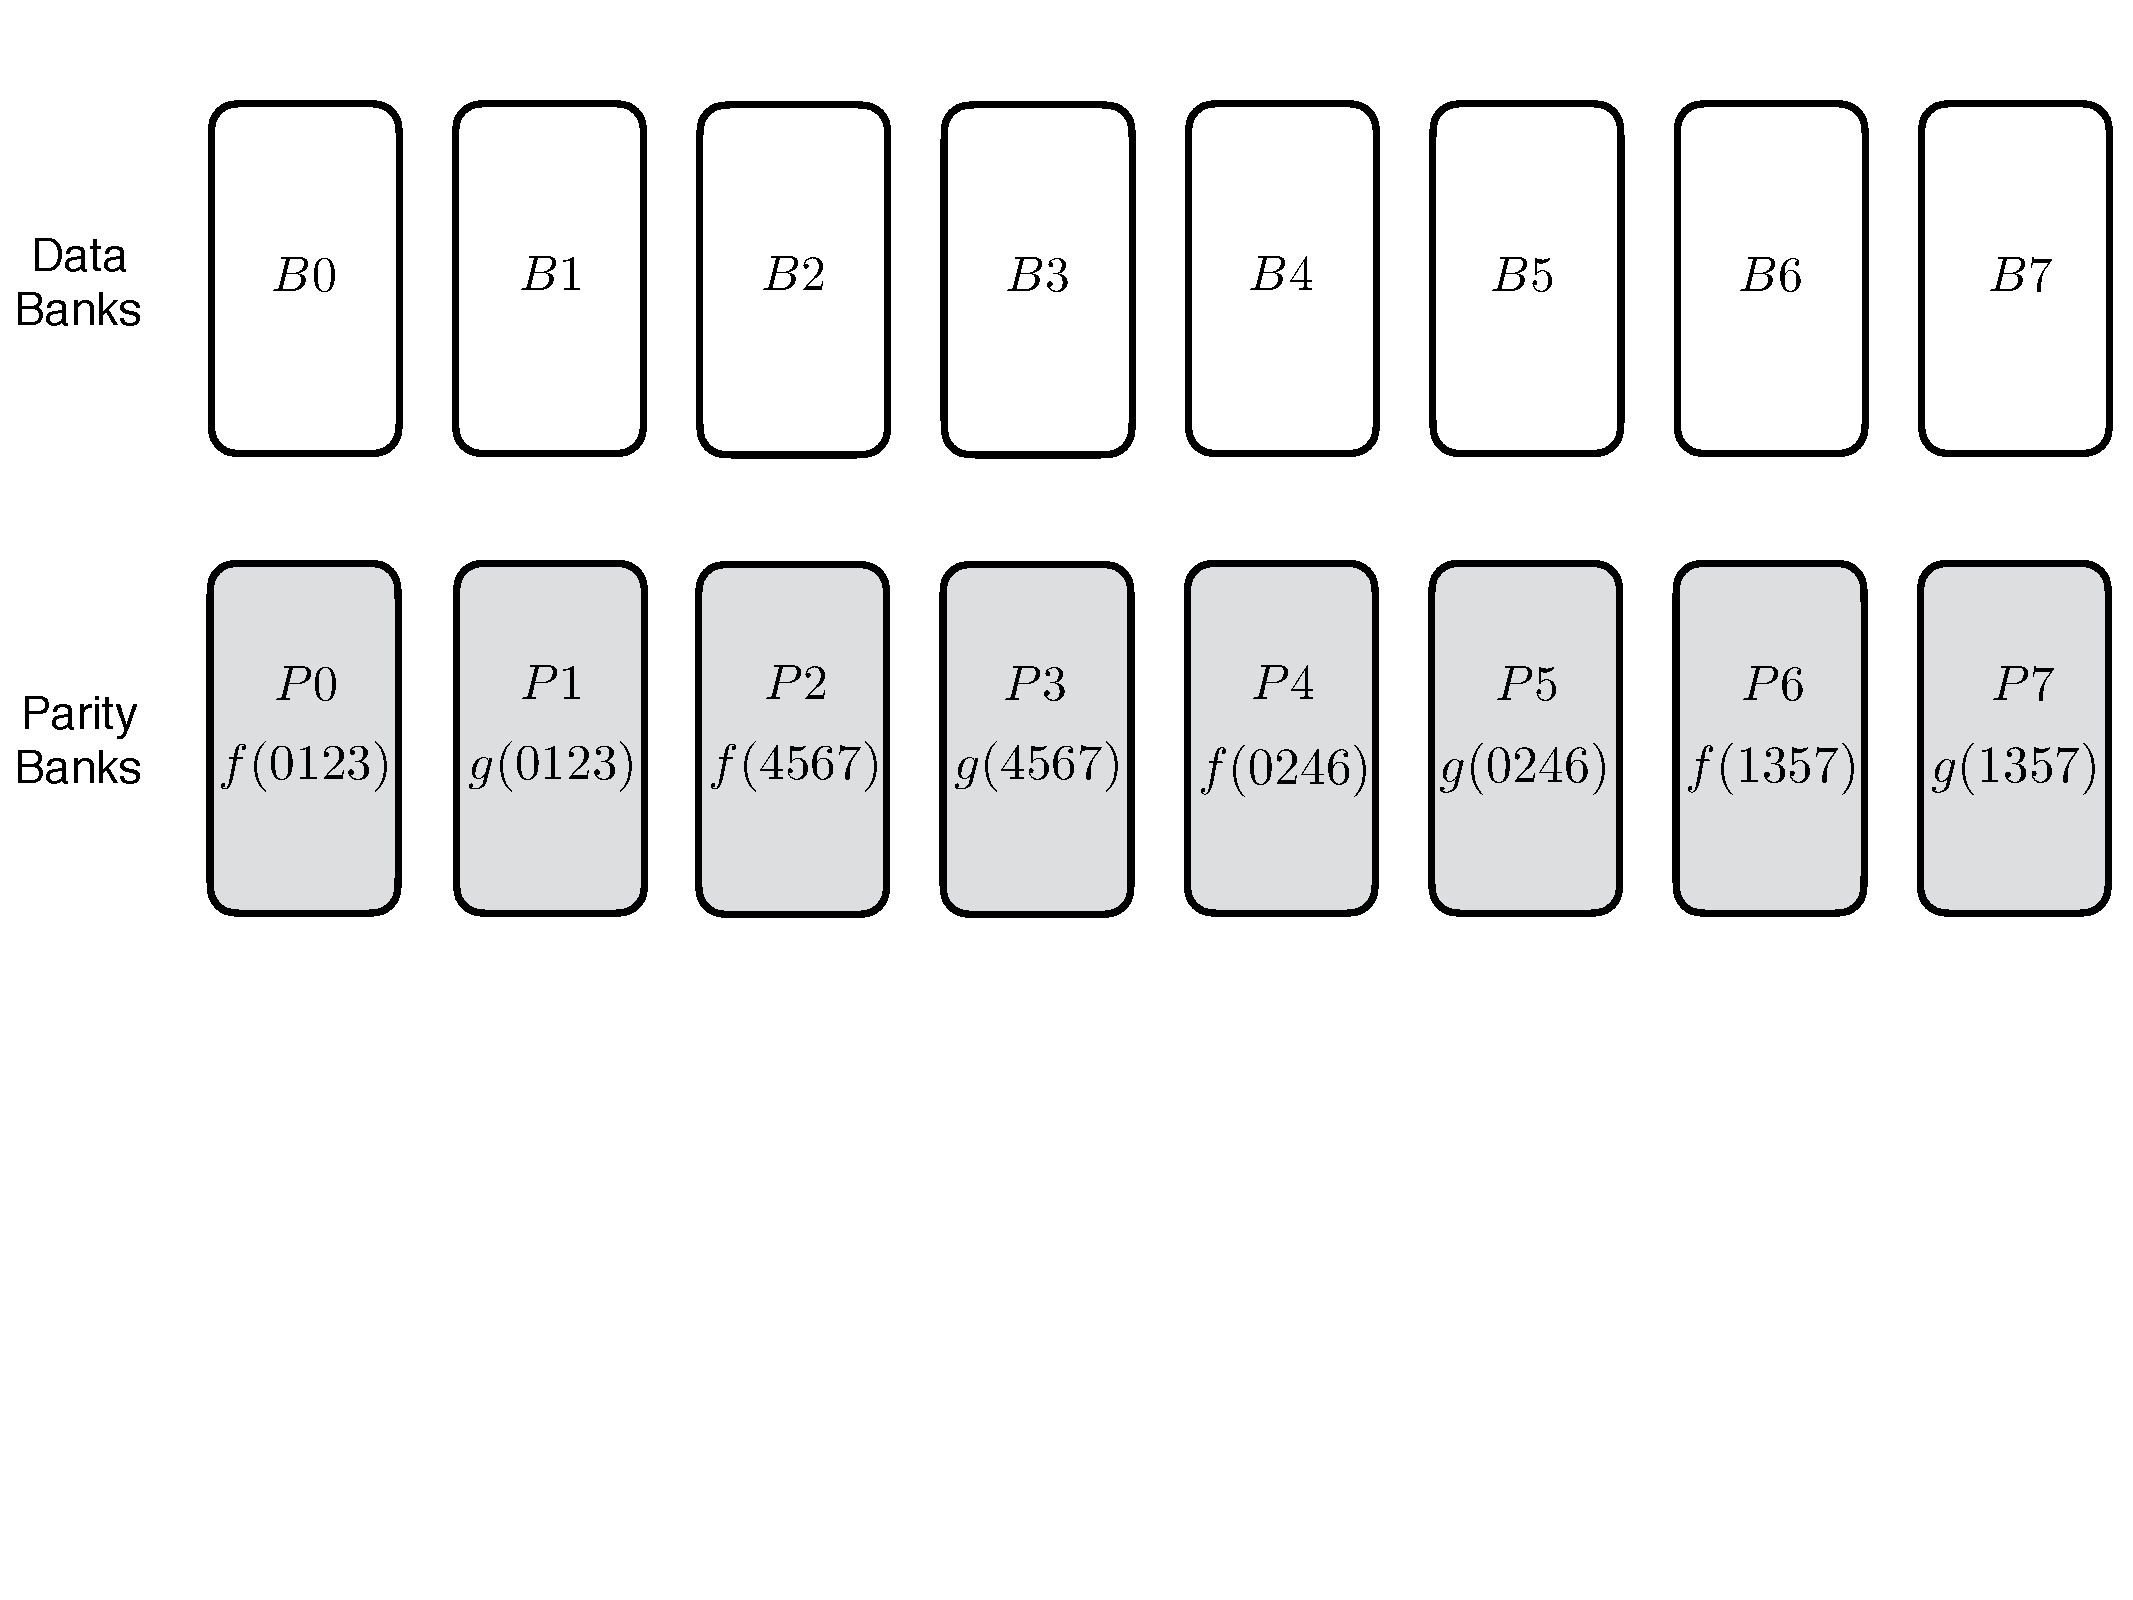
\includegraphics[width=0.7\linewidth]{figures/Code-Design.pdf} 
\caption{Data storage layout for coded memory system}
\label{fig:memsys}
\end{figure*}


\section{CODED MEMORY SYSTEM}
\label{sec:codingArchitecture}

In this paper, we aim to extend the benefits of coding theoretic techniques to dynamic random-access memory systems. In particular, we achieve this by storing the information across single port memory banks in a redundant manner. Traditionally, when multiple requests to a single bank are issued by the cores, a stall occurs as only one address from a single bank can be accessed at a time. As a result, the cores must wait for the first request to the bank be served before their other requests to the bank can be processed. This is where a redundant storage space based on a carefully designed coding scheme comes to the rescue. During a given memory cycle, any data bank that is blocked/busy serving an access can be viewed as a failure as far as other accesses are concerned. Now, other accesses intended for this blocked bank can be served by accessing the content stored in a group of other memory banks. This way, redundant storage space allows concurrent accesses to the same information and alleviates the stalls that are unavoidable in a memory system comprised of non-redundant storage space. 

In this section, we describe our specific memory design in detail. First, we present how to use Reed-Solomon codes to introduce redundancy in the memory storage space. We then discuss the memory controller, the other essential block of our design. Our proposed controller exploits memory bank redundancies to reduce the effect of concurrent read accesses to the stored information. Additionally, the memory controller also maintains consistency and validity of the stored data, which arises due to the presence of write accesses. 




\subsection{Coded Multi-bank Storage Space}
\label{sec:codedBanks}

We rely on a systematic Reed-Solomon (RS) coding scheme as a building block to design the storage space of our proposed memory system. In particular, the storage space consists of $16$ memory banks\footnote{We believe that a $16$ bank design is quite reasonable given that the next generation memory architectures feature many more memory banks than current DRAM architectures.} with $8$ memory banks serving as the data banks and the remaining $8$ banks serving as the parity banks (cf.~Section~\ref{sec:encoding}). As detailed later in this subsection, the parity banks are generated using a systematic $(6,4)$ RS code which is defined over a finite field of size $2^8$, denoted by $GF(2^{8})$.  In any codeword of this systematic $(6,4)$ RS code, it's possible to generate all $4$ associated message symbols given any $4$ symbols of the codeword. 

Before we describe the process of generating the parity blocks, we discuss the reasons behind employing RS codes as opposed to other possible coding schemes. First, RS codes are MDS codes (cf.~Section~\ref{sec:block-codes}), i.e., these codes are optimal in terms of their storage efficiency. 
 Additionally, decades of study has lead to efficient encoding and decoding schemes for RS codes. Crucially, these schemes can be easily \textit{hardcoded} into the memory controller in order to achieve good runtime performance. Finally, RS codes have been proven to be useful in previous work on distributed storage, both in theory and in practice \cite{huang,sathiamoorthy,shanmugam}. In fact, $(14,10)$-RS code is used in production at Facebook in their HDFS-RAID system \cite{sathiamoorthy}. This makes these codes a natural starting point for our dense memory storage architecture.

We now describe the detailed design of the storage space of our proposed memory system. Let the underlying systematic $(6,4)$ RS code map $4$ message symbols $u, v, w, x \in GF(2^{8})$ to a codeword containing $6$ symbols 
$$
\big(u, v, w, x, f(u, v, w, x), g(u, v, w, x)\big) \in GF(2^{8})^6,
$$
where $f, g~:~GF(2^{8})^4 \to GF(2^{8})$ are two linear maps. We arrange the information in $8$ data banks $B0, B1, \ldots, B7$ as shown in Figure~\ref{fig:memsys}. The parity banks $P0, P1,\ldots, P7$ then store the parity symbol which are generated according to the $(6,4)$ RS code described above\footnote{Recall the encoding process and associated notation defined in Section~\ref{sec:encoding}. For example, the functions $f$ and $g$ are applied to the symbols stores in a given row address of $B0, B1, B2,$ and $B3$ to obtain the symbols stored in the same row address of the parity banks $f(0123) \triangleq f(B0,B1,B2,B3)$ and $g(0123) \triangleq g(B0, B1, B2, B3)$, respectively.}. In particular, the first two parity banks $P0$ and $P1$ store the parity symbols that are functions of the information stored in the first four data banks $B0, B1, B2,$ and $B3$. Note that this implies that the symbols stored on the same row address of the six banks $\{B0,\ldots, B3, P0,P1\}$ form codewords of the underlying $(6,4)$ RS code. Similarly, the parity symbols generated from the remaining four data banks $B4, B5, B6,$ and $B7$ are stored in the parity banks $P2$ and $P3$. 

In our design, we ensure that each data bank is part of $2$ codewords of the $(6,4)$ RS code, which are formed by disjoint sets of parity banks. This creates disjoint ways of recovering the information stored in the same data bank. We utilize the parity banks $P4, P5, P6,$ and $P7$ to generate the second codewords associated the data banks. In particular, parity banks $P3$ and $P4$ store the parity symbols generated from the information stored on the even numbered data banks $B0, B2, B4,$ and $B6$. Similarly, the parity banks $P6$ and $P7$ store the parity symbols generated from the odd numbered data banks $B1, B3, B5,$ and $B7$. 

\begin{remark}
\label{rem:degraded}
Note that the redundancy in the storage space helps enable concurrent read accesses by treating the blocked data banks as failures. For example, assume that $B0$ and $B1$ are blocked due to some read accesses. Now, another read access to $B0$ can be realized by using $B2, B3, P0 = f(B0, B1, B2, B3),$ and $P1 = g(B0, B1, B2, B3)$ to recover the symbol in $B0$ required by the access. Similarly, consider a different scenario, where $B0$ is busy serving a read access. Now, another read access for the information stored in $B0$ can be served by reconstructing that information with the help of three data banks $B1, B2, B3,$ and one parity bank $P0 = f(B0, B1, B2, B3)$ or $P1 = g(B0, B1, B2, B3)$.
\end{remark}

%\Ankit{Please somebody rewrite these two lines and then put them in right place...} {\color{blue}The upper part of the bank stores Pseudo Channel 0, and the lower part of the bank stores Pseudo Channel 1. 
%Wherever possible, we try to interleave the banks. This ensures that most large, linear accesses will be spread across multiple banks with reduced contention.}


\subsection{Memory Controller Design}
\label{sec:controller}
The proposed architecture of the memory controller consists of a scheduler which converts memory access requests from the cores into memory access patterns that are mapped to different memory banks. The scheduler has three main components: 1) {\em reorder buffer}, 2) {\em read algorithm}, and 3) {\em write algorithm}. The reorder buffer stores the list of pending or recently served access requests by the memory system. In addition, the reorder buffer also keeps track of the status of the data stored on memory banks as it gets {\em stale} ({\em invalid}) as a result of write requests. The scheduler compares each read and write request to the content of the reorder buffer in order to decide how the request gets served by the read algorithm and the write algorithm, respectively. Next, we describe each of these three main components of the memory controller in detail. 
Table~\ref{fig:rob} shows the behavior of our proposed memory controller architecture on an example request pattern.
%
%\begin{table*}[t!]
% \small
%  \centering
%  \begin{tabular}{c|c|c|c|c|c|c|c|c|c|c|c|c|c|c|c|l}
%    \cline{2-16}
%&    $ROW$ & $Done$ & $R/W$ & $D_{\rm valid}$ & $P_{\rm valid}$ & $DB_{0}$ &  $DB_{1}$ & $DB_{2}$ &$\cdots$ & $DB_7$  & $PB_0$ &  $PB_{1}$ & $PB_{2}$ & $\cdots$ & $PB_7$ \\
%    \cline{2-16}
%t=$1$ &   \texttt{0x2} & 0 & R  & 0 & 0  & 1 & 1 & 0 & 0 & 0 & 0 & 0  & 0 & 0& 0 & {\scriptsize Read $DB_0 - DB_1$}\\
%    \cline{2-16}
%t=$2$ &    \texttt{0x2} & 0 & R & 1 & 1 & 1 & 1 & 1 & 1& 1 & 1& 1 &1 &1&1& {\scriptsize Read $DB_0 - DB_7$}\\
%   \cline{2-16}                          
%t=$3$ &    \texttt{0x2} & 0 & W & 0 & 0 & 0 & 1 & 1 & 1& 1 & 0 & 0 & 0 & 0 & 0 & {\scriptsize Write $DB_0$} \\
%   \cline{2-16}                          
%t=$4$ &    \texttt{0x2} & 0 & W & 1 & 0 & 1 & 1 & 1 & 1& 1 & 0 & 0 & 0 & 0 & 0& \\
%    \cline{2-16}   
%t=$5$ &    \texttt{0x2} & 0 & R & 1 & 0 & 1 & 1 & 1 & 1& 1 & 0 & 0 & 0 & 0 & 0 & {\scriptsize Read $DB_4 - DB_6$}\\
%    \cline{2-16} 
%t=$6$ &    \texttt{0x2} & 1 & R & 1 & 1 & 1 & 1 & 1 & 1& 1 & 1 & 1 & 1 & 1 & 1 &\\
%    \cline{2-16} 
%t=$7$ &    \texttt{0x2} & 1 & R & 1 & 1 & 1 & 1 & 1 & 1& 1 & 1 & 1 & 1 & 1 & 1 &{\scriptsize Read $DB_0 - DB_7$} \\
%    \cline{2-16}                                                     
%  \end{tabular}
%  \caption{Example of a single entry \texttt{0x2} in the reorder buffer across time during a Read-Write-Read request pattern. At t=$1$, there is a read from $DB_0$--$DB_1$, followed by a read at $t=2$ from $DB_0$--$DB_7$ which includes both data and parity banks. A write request to $DB_0$ occurs from $t=3$ to $t=6$, during which $DB_0$ is updated, $D_{\rm valid}$ is set to $1$,  parities $PB_0$--$PB_7$ are updated, $P_{\rm valid}$ is set to $1$, and $Done$ is set to $1$. Since data banks are valid after $t=4$, a read from $DB_{4} $--$DB_6$ is served using only data banks at $t=5$, which sets the $R/W$ bit to $R$. A read from $DB_0 $--$DB_7$ occurs at $t=7$, which does not change the state of the reorder buffer.}
%  \label{fig:rob}
%\end{table*}

\begin{table*}[t!]
 \small
  \centering
  \begin{tabular}{c|c|c|c|c|c|c|c|c|c|c|c|c|c|c|c|l}
    \cline{2-16}
&    $ROW$ & $Done$ & $R/W$ & $D_{\rm valid}$ & $P_{\rm valid}$ & $DB_{0}$ &  $DB_{1}$ & $DB_{2}$ &$\cdots$ & $DB_7$  & $PB_0$ &  $PB_{1}$ & $PB_{2}$ & $\cdots$ & $PB_7$ \\
    \cline{2-16}
t=$1$ &   \texttt{0x2} & 0 & R  & 0 & 0  & 1 & 1 & 0 & 0 & 0 & 0 & 0  & 0 & 0& 0 & {\scriptsize Read $B0 - B1$}\\
    \cline{2-16}
t=$2$ &    \texttt{0x2} & 0 & R & 1 & 1 & 1 & 1 & 1 & 1& 1 & 1& 1 &1 &1&1& {\scriptsize Read $B0 - B7$}\\
   \cline{2-16}                          
t=$3$ &    \texttt{0x2} & 0 & W & 0 & 0 & 0 & 1 & 1 & 1& 1 & 0 & 0 & 0 & 0 & 0 & {\scriptsize Write $B0$} \\
   \cline{2-16}                          
t=$4$ &    \texttt{0x2} & 0 & W & 1 & 0 & 1 & 1 & 1 & 1& 1 & 0 & 0 & 0 & 0 & 0& \\
    \cline{2-16}   
t=$5$ &    \texttt{0x2} & 0 & R & 1 & 0 & 1 & 1 & 1 & 1& 1 & 0 & 0 & 0 & 0 & 0 & {\scriptsize Read $B4 - B6$}\\
    \cline{2-16} 
t=$6$ &    \texttt{0x2} & 1 & R & 1 & 1 & 1 & 1 & 1 & 1& 1 & 1 & 1 & 1 & 1 & 1 &\\
    \cline{2-16} 
t=$7$ &    \texttt{0x2} & 1 & R & 1 & 1 & 1 & 1 & 1 & 1& 1 & 1 & 1 & 1 & 1 & 1 &{\scriptsize Read $B0 - B7$} \\
    \cline{2-16}                                                     
  \end{tabular}
  \caption{Example of a single entry \texttt{0x2} in the reorder buffer across time during a Read-Write-Read request pattern. At t=$1$, there is a read from $B0$--$B1$, followed by a read at $t=2$ from $B0$--$B7$ which includes both data and parity banks. A write request to $B0$ occurs from $t=3$ to $t=6$, during which $DB_0$ is updated, $D_{\rm valid}$ is set to $1$, bits for parities banks, i.e., $PB_0$--$PB_7$, are updated, $P_{\rm valid}$ is set to $1$, and $Done$ is set to $1$. Since data banks are valid after $t=4$, a read from $B{4} $--$B6$ is served using only data banks at $t=5$, which sets the $R/W$ bit to $R$. A read from $B0 $--$B7$ occurs at $t=7$, which does not change the state of the reorder buffer. \Matt{Why does writing to B0 set all PB bits to 0? not all parity banks are a function of B0.}}
  \label{fig:rob}
\end{table*}

\subsubsection{Reorder buffer}
\label{sec:reorder}

As mentioned earlier, all access requests need to go through the reorder buffer. The reorder buffer stores the data downloaded from the memory banks in order to serve read access requests from the cores. Similarly, the reorder buffer also stores the new data that arrives with write requests and need to be written on the coded memory banks (after generation of consistent parity data). In addition to storing the actual data, the reorder buffer maintains metadata to keep track of the rows of the memory banks that are present in the reorder buffer and the validity of these rows across data banks and parity banks. Each write request invalidates the content of (some of) the data banks. The data on these banks (and on the corresponding parity banks which depend on them) then needs to be updated. The metadata of the reorder buffer is used to ensure this consistency across the data and parity banks when the memory controller maps a write request to be written on the memory banks. The reorder buffer size is a key design parameter which trades off faster access speeds for increased overhead, as shown in Section~\ref{sec:experiments}.


For each row address in the memory banks, the reorder buffer stores {\em at most $1$} entry along with the following $20$ bits of metadata (cf.~Table~\ref{fig:rob}). 
\begin{itemize}
\item {$Done$:~}This bit indicates if this particular row address had a write request associated with it in the past that has not yet been written to the memory banks. If $Done$ bit is set to $1$, this implies that this row address was affected by the write requests and the content on the memory banks need to be updated when this row is removed from the metadata of the reorder buffer.
\item {$R/W$:~} This bit denotes the nature of the most recent access request for the row address associated with the entry in reorder buffer. $R$ and $W$ refers to the read request and the write request, respectively.
\item {$D_{\rm valid}$:~}This bit indicates if the reorder buffer stores the valid data for the corresponding row address in each of the {\em data} banks. $D_{\rm valid}$ bit is set to $1$ when the reorder buffer has the valid copies of the content for all the data banks.
\item {$P_{\rm valid}$:~}This bit indicates if the reorder buffer stores the valid data for the corresponding row address in each of the {\em parity} banks. $P_{\rm valid}$ bit is set to $1$ when the reorder buffer stores the valid copies of the data for all the parity banks.
\item {$DB_0, \ldots, DB_7$:~}Similar to the $D_{\rm valid}$ bit, for $0 \leq i \leq 7$, $DB_{i}$ bit is set to $1$ to denote that the reorder buffer stores the valid data for the associated row address in the $i$-th data bank $Bi$.
\item {$PB_0, \ldots, PB_7$:~}Similar to the $P_{\rm valid}$ bit, for $0 \leq i \leq 7$, $PB_{i}$ bit is set to $1$ to indicate that the reorder buffer stores the valid version of the content for the associated row address in the $i$-th parity bank $Pi$.
\end{itemize}
Note that $D_{\rm valid}$ and $P_{\rm valid}$ are logical $AND$s  of $DB_{0}-DB_{7}$ and $PB_{0}-PB_{7}$, respectively. 
\begin{remark}
Even though the data stored in a particular row in the memory banks might be invalid, the reorder buffer may store its valid version which would lead to the $D_{\rm valid}$ and/or $P_{\rm valid}$ bits to be set. It's the responsibility of the write algorithm to transfer this valid data from the reorder buffer to the memory banks when the corresponding row is evicted from the reorder buffer.
\end{remark}

\begin{remark}
\label{rem:priority}
Here, we note that the reorder buffer can also be utilized to incorporate different priority levels among access requests, if the memory systems is required to support multiple access types with different priority levels.
\end{remark}


\subsubsection{Read algorithm}
\label{sec:read}

For a given state of the reorder buffer and the set of pending read requests from the cores, the main purpose of the read algorithm is to maximize the number of read requests that can be served in a given memory cycle. This is accomplished by utilizing the redundant parity banks in an efficient manner without increasing the algorithm's overall complexity. Note that in our coded memory design (cf.~Section~\ref{sec:codedBanks}), a parity bank is useful during data access only if some of the corresponding data banks are also accessed. In particular, assuming that all the relevant parity banks are valid, there are two possible ways of serving a read request by employing the parity banks: 1) content of $2$ data banks and $2$ parity banks is utilized; and  2) content of $3$ data banks and $1$ parity bank is utilized (cf.~Remark~\ref{rem:degraded}). In every cycle, the scheduler picks pending read requests {\em in order} and tries to serve them according to the read algorithm described in Figure~\ref{fig:read}. In addition to this, whenever all but $1$ data bank is present in the buffer, that data bank is automatically read from memory and the algorithm proceeds with $D_{\rm valid}$ set to $1$. \Matt{Read algorithm questions:
1) Where is the R/W bit set to read?
2) Regarding the $D_{valid} = true$ condition, Why does $D_{valid}$ need to be true to serve a request? Say I want to read from B0, and the DB0 bit is set. There is enough information in the Reorder buffer to serve the request. Why should I care if $D_{valid}$ is set?}
%-------------------------------------------------------------------------
\begin{figure}[h!] \centering
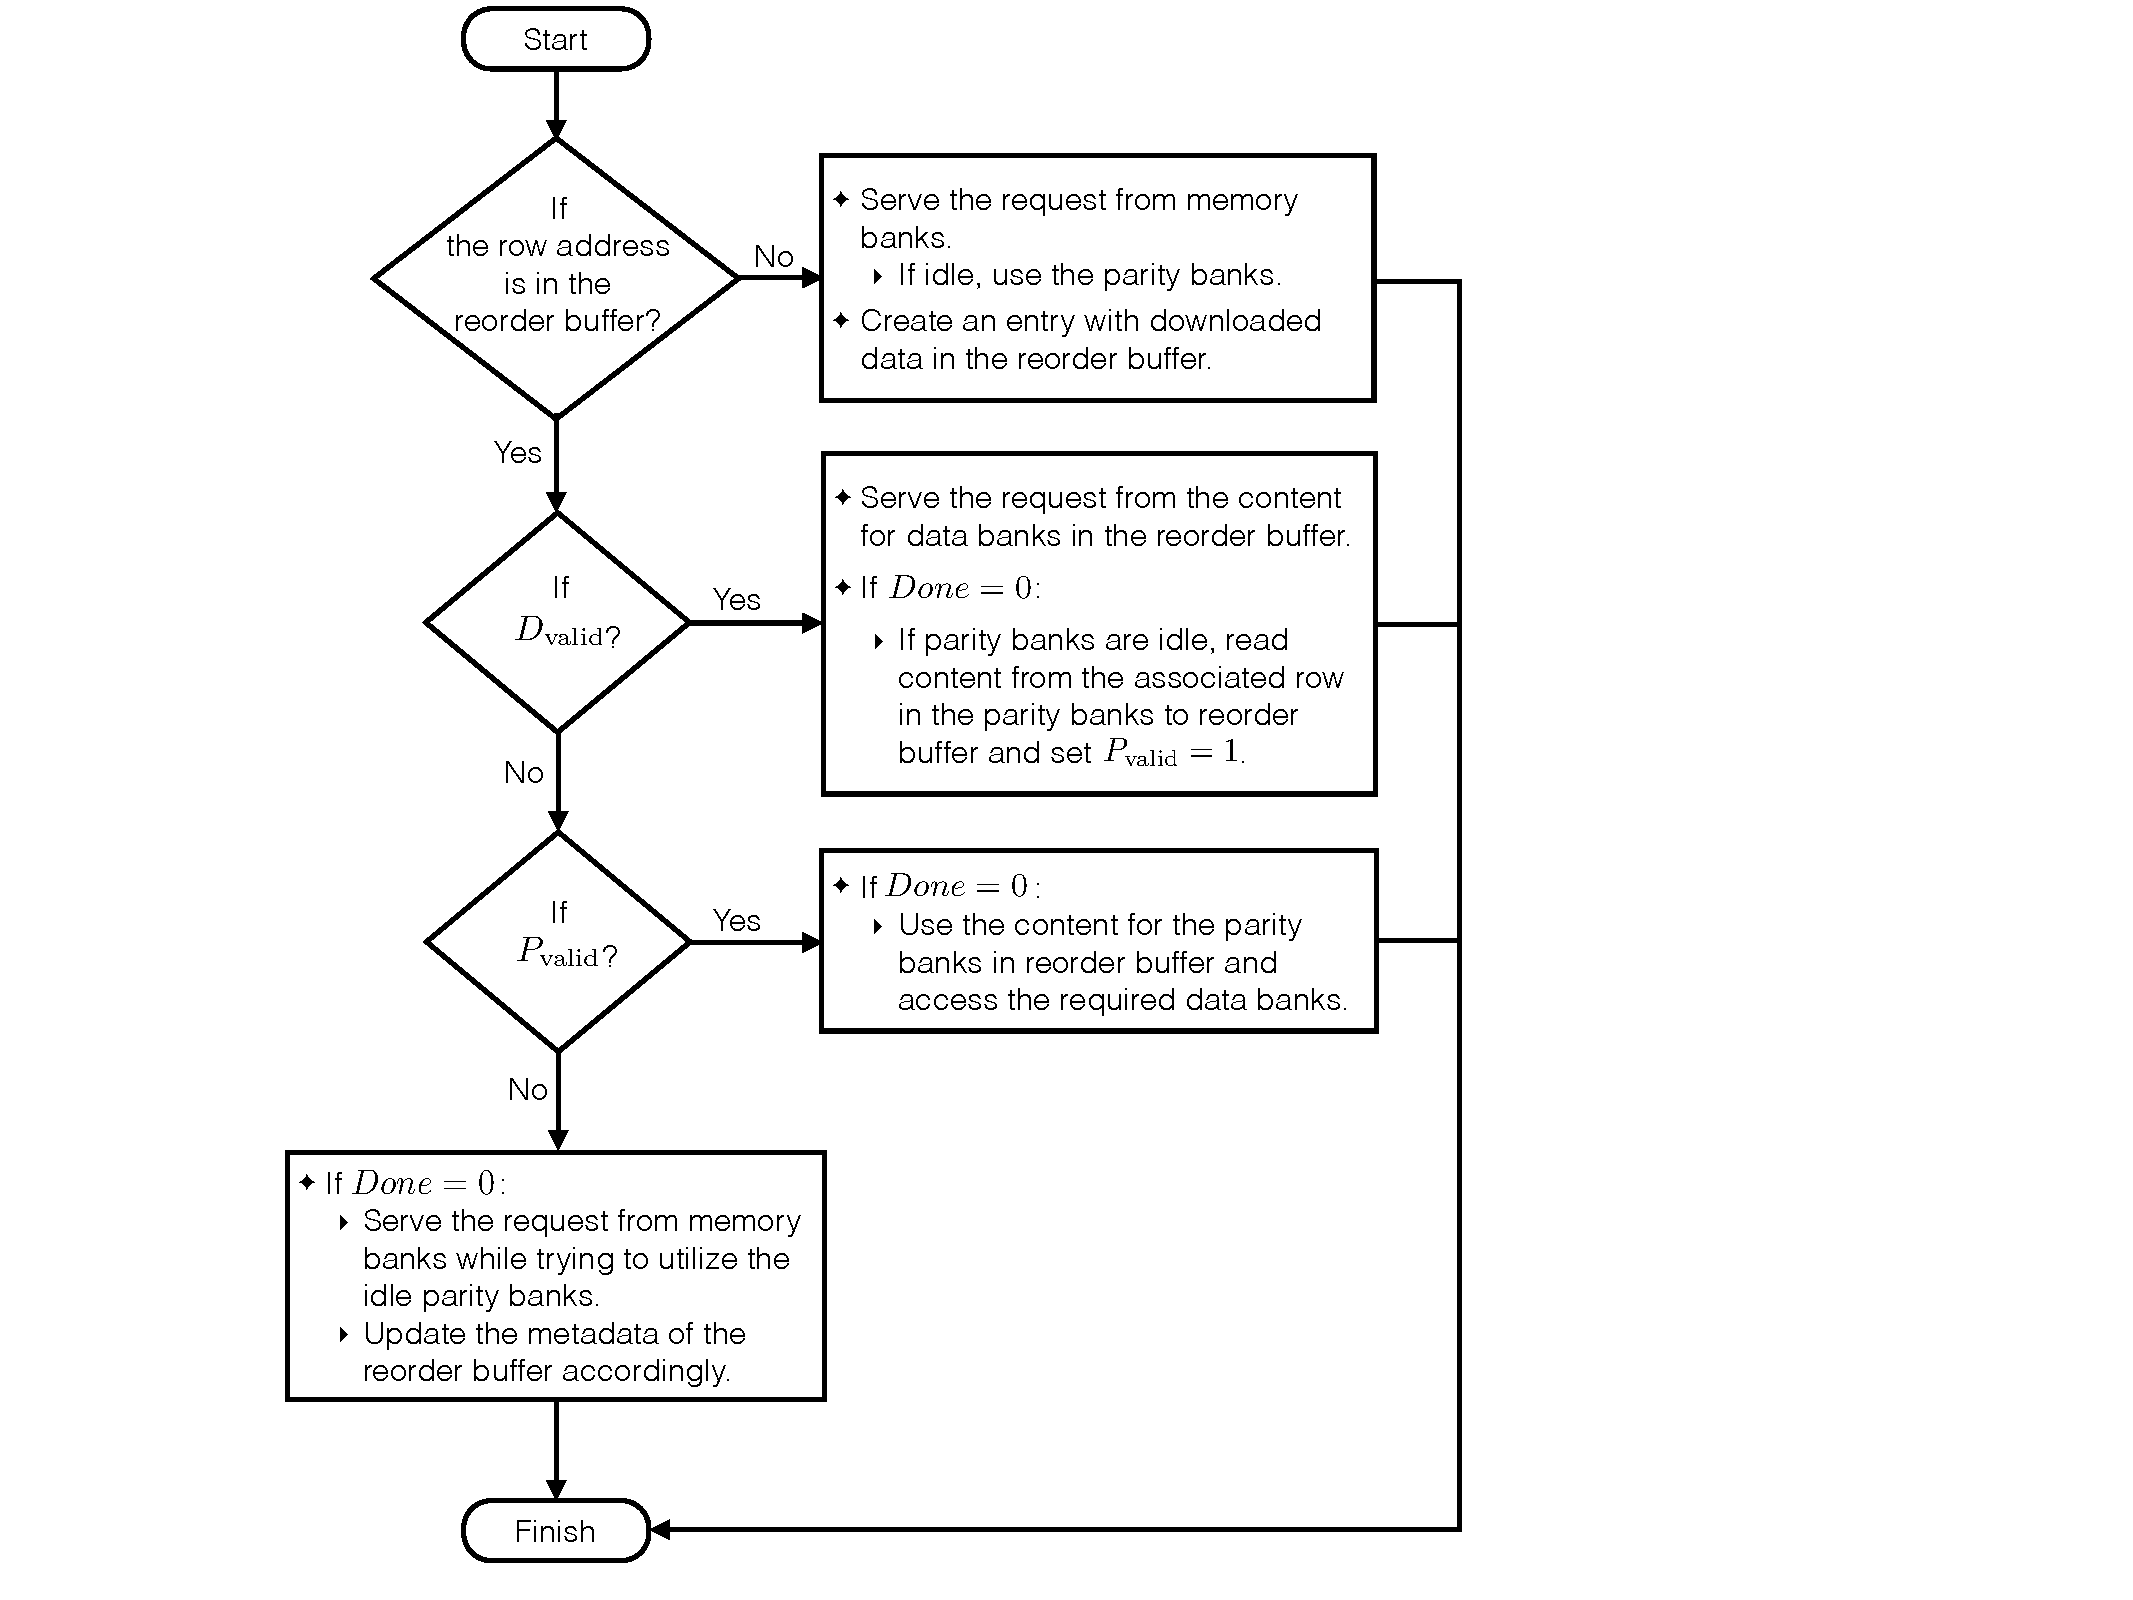
\includegraphics[width=0.85\linewidth]{figures/Read-algo-new.pdf} 
\caption{Description of the read algorithm.}

\label{fig:read}
\end{figure}
%-------------------------------------------------------------------------

\subsubsection{Write algorithm}
\label{sec:write}
Note that each write request is accompanied by the content that needs to be updated in (some of) the data banks. However, in order to have consistency across all the memory banks, every update in the data banks should be reflected in the associated parity banks as well. The write algorithm ensures that the reorder buffer stores consistent and valid data for each row address available in the buffer. The write algorithm achieves this task by following the procedure described in Figure~\ref{fig:write}. In particular, the write algorithm picks the pending write access requests from the core in order. The algorithm then determines if the associated row address is present in the reorder buffer. If it is not present, it makes an entry for the row in the reorder buffer. \Matt{Why set every parity bank bit to 0 when performing a write? Suppose you write to DB0. That shouldn't effect parity banks which are not functions of DB0}

\begin{figure}[h!] \centering
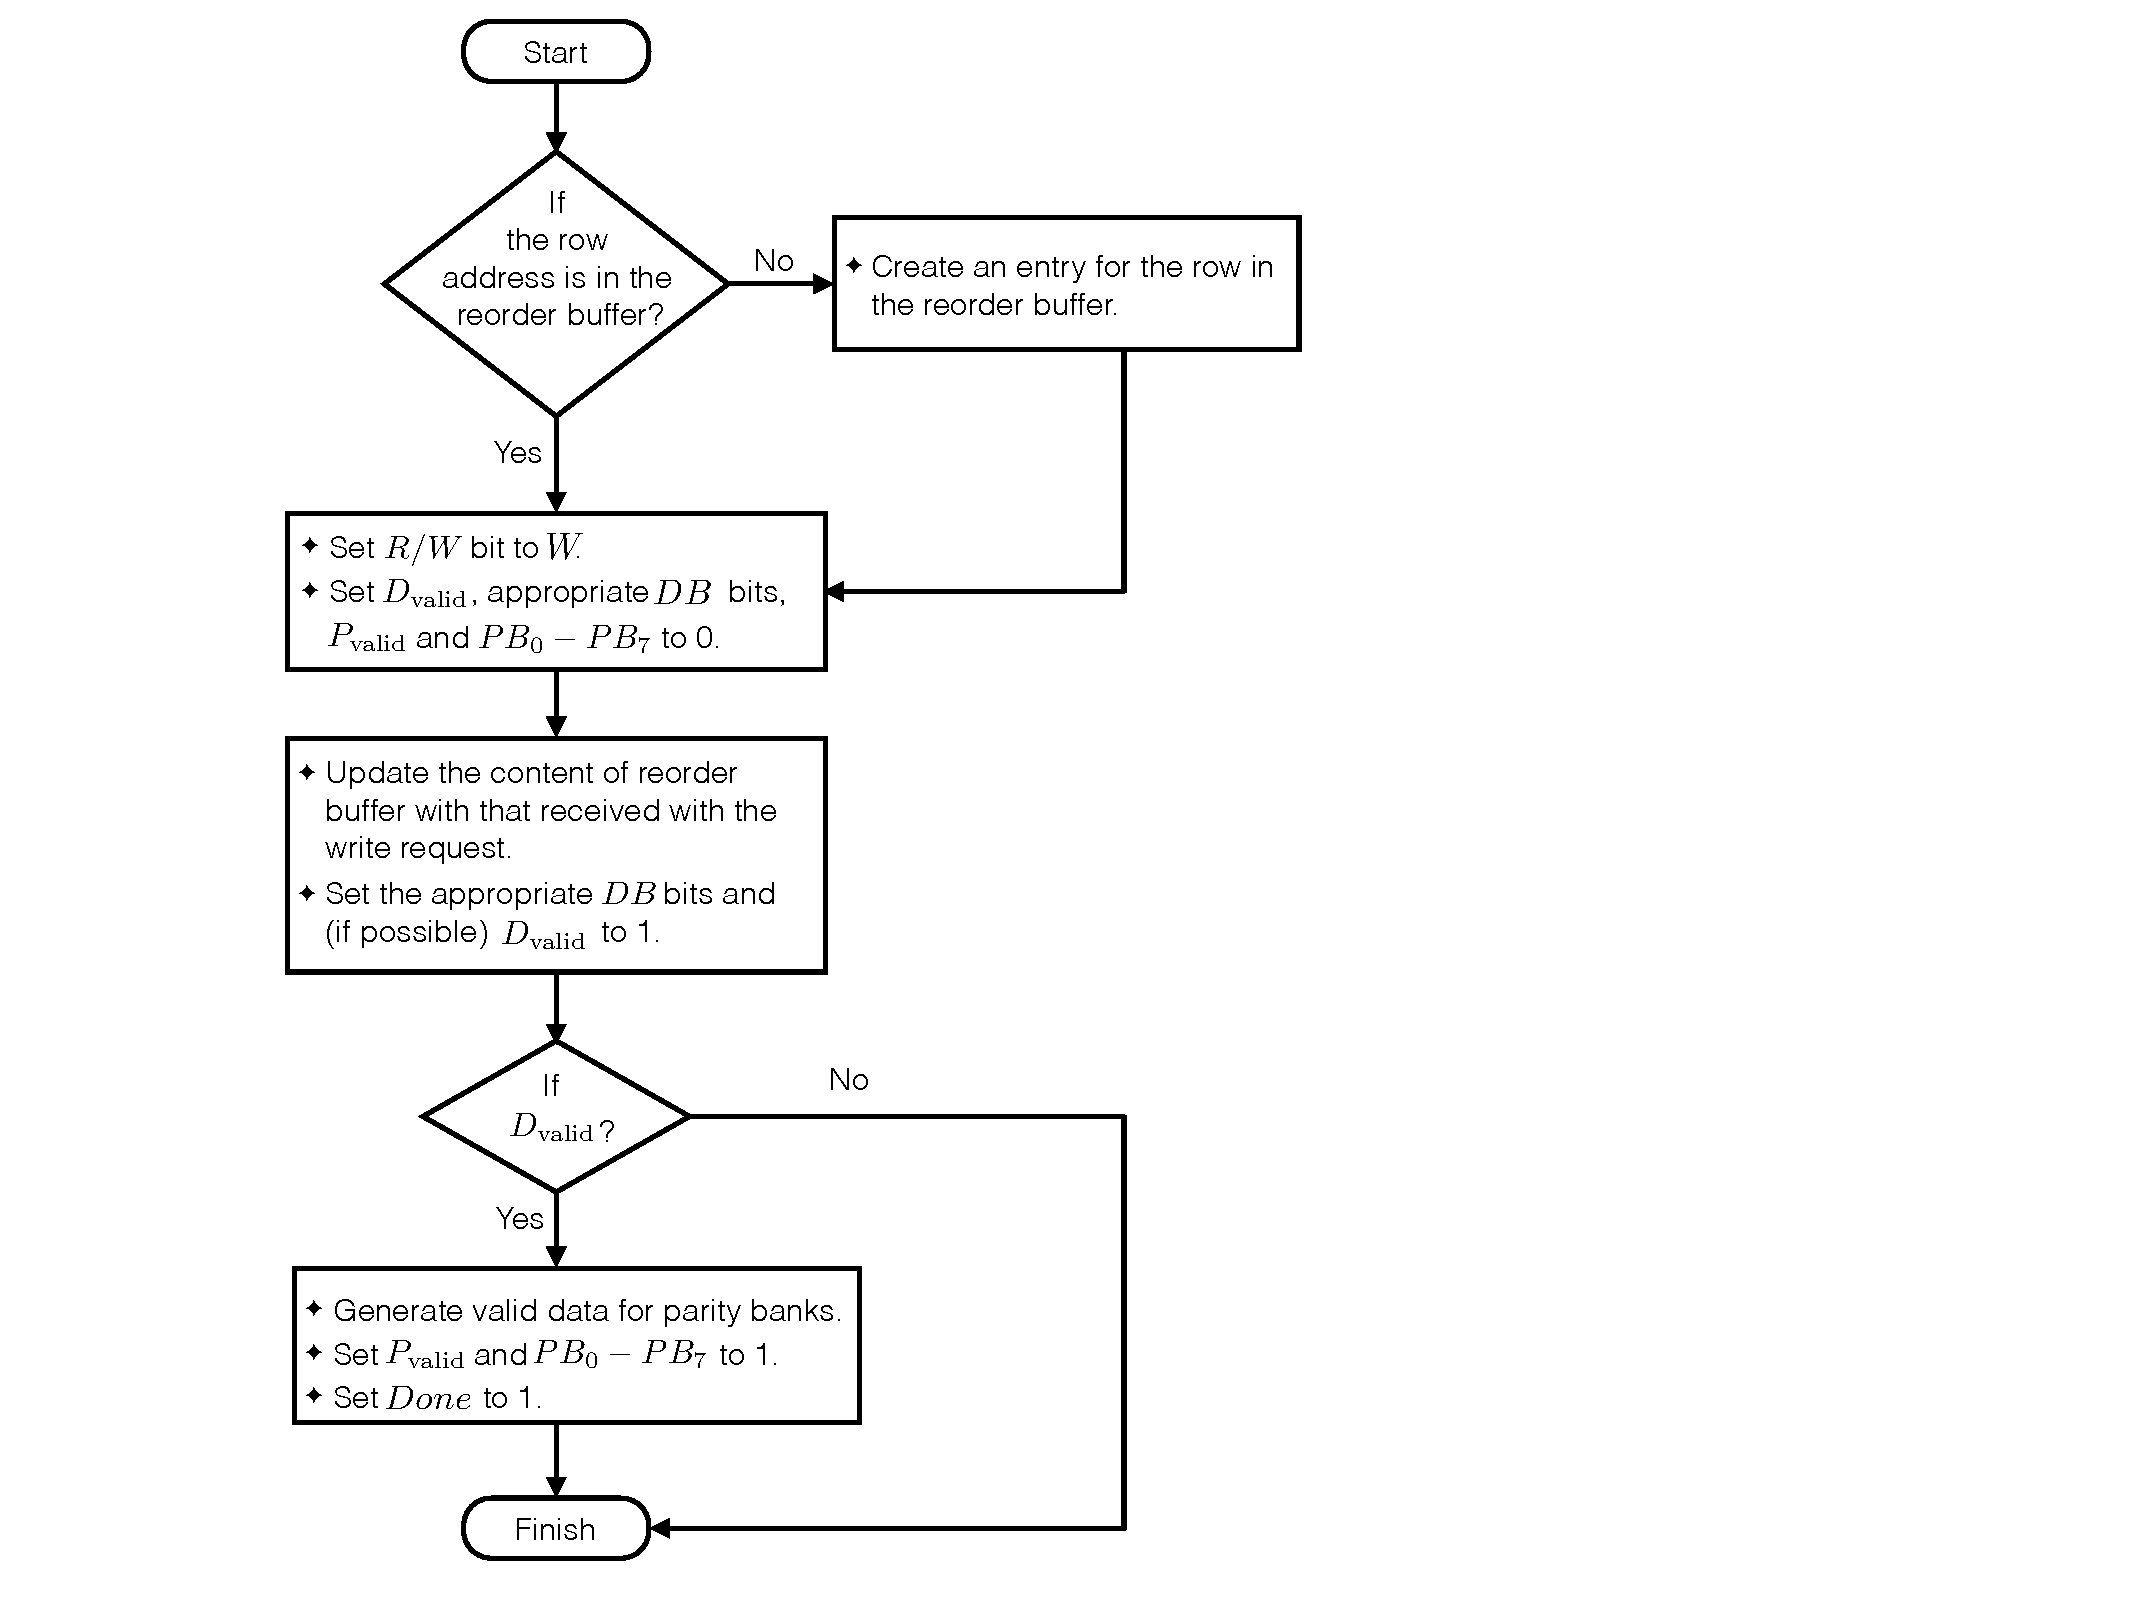
\includegraphics[width=0.80\linewidth]{figures/Write-algo-new.pdf} 
\caption{Description of the write algorithm.}
\label{fig:write}
\end{figure}


Once the reorder buffer has the entry for the row address, the write algorithm ensures that the buffer stores the valid content for the row address. This involves 1) copying the content received with the write request to update the content already available in the buffer from the data banks; 2) regenerating the updated content for the parity banks; and 3) updating the metadata of reorder buffer by modifying the entry corresponding to the underlying row address. Once the reorder buffer has valid and consistent data for a given row address, $Done$ is set to $1$. 

Table~\ref{fig:rob} illustrates these steps for an example write request. At $t = 3$, the write algorithm starts processing a write request for data bank $B0$ by setting the $R/W$ bit with the associated address to $W$. It also sets the $D_{\rm valid}$, $DB_{0}$, $P_{\rm valid}$ and $PB_{0}-PB_{7}$ to zero. In the subsequent steps, the write algorithm updates the content for data bank $B0$ in the buffer by replacing it with the content received with the write request. It then updates $DB_0$ and $D_{\rm valid}$ by setting those to $1$. If $D_{\rm valid}$ is $0$, the reorder buffer entry remains in the buffer until all data banks are updated. Once $D_{\rm valid}$ is indeed $1$, then the write algorithm generates the new content for the parity banks and sets $P_{\rm valid}$ and $PB_0 -PB_7$ to $1$. At this point, it also sets $Done$ to $1$.

Once the $Done$ bit is set to $1$, the write algorithm schedules the updated row to be written to the memory banks. Once the write is successfully performed on the memory banks, the entry in the reorder buffer is updated by setting $R/W$ bit to $R$ and $Done$ bit to $0$. Here, we note that the $R/W$ bit can get modified by a subsequent read request (as illustrated in Table~\ref{fig:rob}). However, the $Done = 1$ bit reminds the scheduler that the memory banks have not yet been updated.


%{\color{red}The write request is now considered successfully processed as far as the writing algorithm is considered. Note that the content stored on the memory banks has not been updated up to this point. This task of performing the updates on memory banks is handled by the writeback algorithm (cf. Section~\ref{sec:writeback}, which is invoked every time an entry is evicted from the reorder buffer.}

\subsubsection{Writeback algorithm}
\label{sec:writeback}
The scheduler uses the limited size reorder buffer to fetch data from the bank rows and to perform read, write and code operations. In the process, the scheduler ensures that every time the reorder buffer reaches near its capacity, it clears up entries based on the following set of rules: Rule 1 is to pop out the oldest entry in the reorder buffer. Rule 2 is to ensure that the evicted row from the reorder buffer matches the data in the memory bank. This is ensured by using the $Done$ bit in the reorder buffer. If a write instruction modifies a data bank entry, the scheduler reconstructs the code and makes $Done = 1$. 

%%%%%%%%%%%%%%%%%%%%%%%%%%%%%%%%%%%%%%%%%%%%%%
% Experiment methodology
%%%%%%%%%%%%%%%%%%%%%%%%%%%%%%%%%
  \section{Experiments}
\label{sec:experiments}

In this section, we describe our HBM implementation and Ramulator simulations on several SPEC2006 benchmarks.

\subsection{HBM Implementation}
%\Ethan{Move all implementation details here, is sub-channel the same as pseudo channel? OK or still repetitive?}
%\Ankit{Suddenly, there is too much jargon about HBM...Have we defined all these things in the background section?}
Our coding scheme is based on a single $16$-bank channel of HBM DRAM operating in Pseudo Channel Mode ($8$ banks per pseudo channel). To fit the layout of Figure~\ref{fig:memsys} and Section~\ref{sec:codingArchitecture}, Pseudo Channel 0 is used for data banks and Pseudo Channel 1 is used for parity banks. 
%
%The pseudo channel conceptually divides the memory of a single channel in half. 
%Since this mode divides a channel into two individual $8$ bank sub-channels, we assign one sub-channel for data banks and the other sub-channel for parity banks. 
%
Wherever possible, we try to interleave the banks. This ensures that most large, linear accesses will be spread across multiple banks with reduced contention.

In this mode, the 128-bit data bus is split into 2 individual 64-bit segments. 
However, the pseudo channels share the same address and command bus: commands and addresses may be sent to one pseudo channel or the other, but not to both. They also decode and execute commands individually. For commands that are common to both pseudo channels, strict timing conditions must be met to avoid conflicts.
%The burst length is set to $4$. This means that on each segment, a read or write transaction transfers $256$ bits in a burst of four $64$-bit cycles. 
Table~\ref{tab:design_params} describes additional design details.
%
\begin{table}[h!]
 \small
  \centering
  \begin{tabular}{|c|p{5cm}|}
    \hline
    Memory overhead & Storage of parity is limited to 50\% of the overall memory. \\
    \hline
    Memory Banks & 8 Data banks, 8 parity banks \\
    \hline           
    Cache Line Size & 128/256 bytes size \\ \hline  
    Element Size & Each element is 256 bytes \\ \hline  
    Number of Cores & 6-8 cores for Wireless SoC platform \\ \hline  
    Access Rate & 1GHz memory speed \\ \hline  
    Burst Length & 4 (256-bit transfer in four 64-bit bursts)\\ \hline
  \end{tabular}
  \caption{Summary table of design parameters.}
  \label{tab:design_params}
\end{table}


\begin{remark} %[{\bf Address mapping}]
\label{rem:address}
%\Ankit{I don't see any reason to present address mapping here...or probably this needs to presented in a better manner to create coherent story.} 
Figure~\ref{fig:mapping} describes the address mapping for each channel. The least significant ``OFFSET'' bits of the address signify the byte level addressing of the data. The $6$ most significant ``CA'' bits indicate column address, the next $14$ ``RA'' bits indicate row address, the $3$ ``BA'' bits decide the bank, and the remaining $3$ ``CH'' bits specify the channel. 
\end{remark}
%%%%%%%%%%%%%%%%%%%%%%%%%%%%%%%%%%%%%%%%%%%
\begin{figure}[h!] \centering
%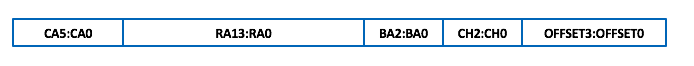
\includegraphics[width=0.95\linewidth]{figures/mapping.png} 
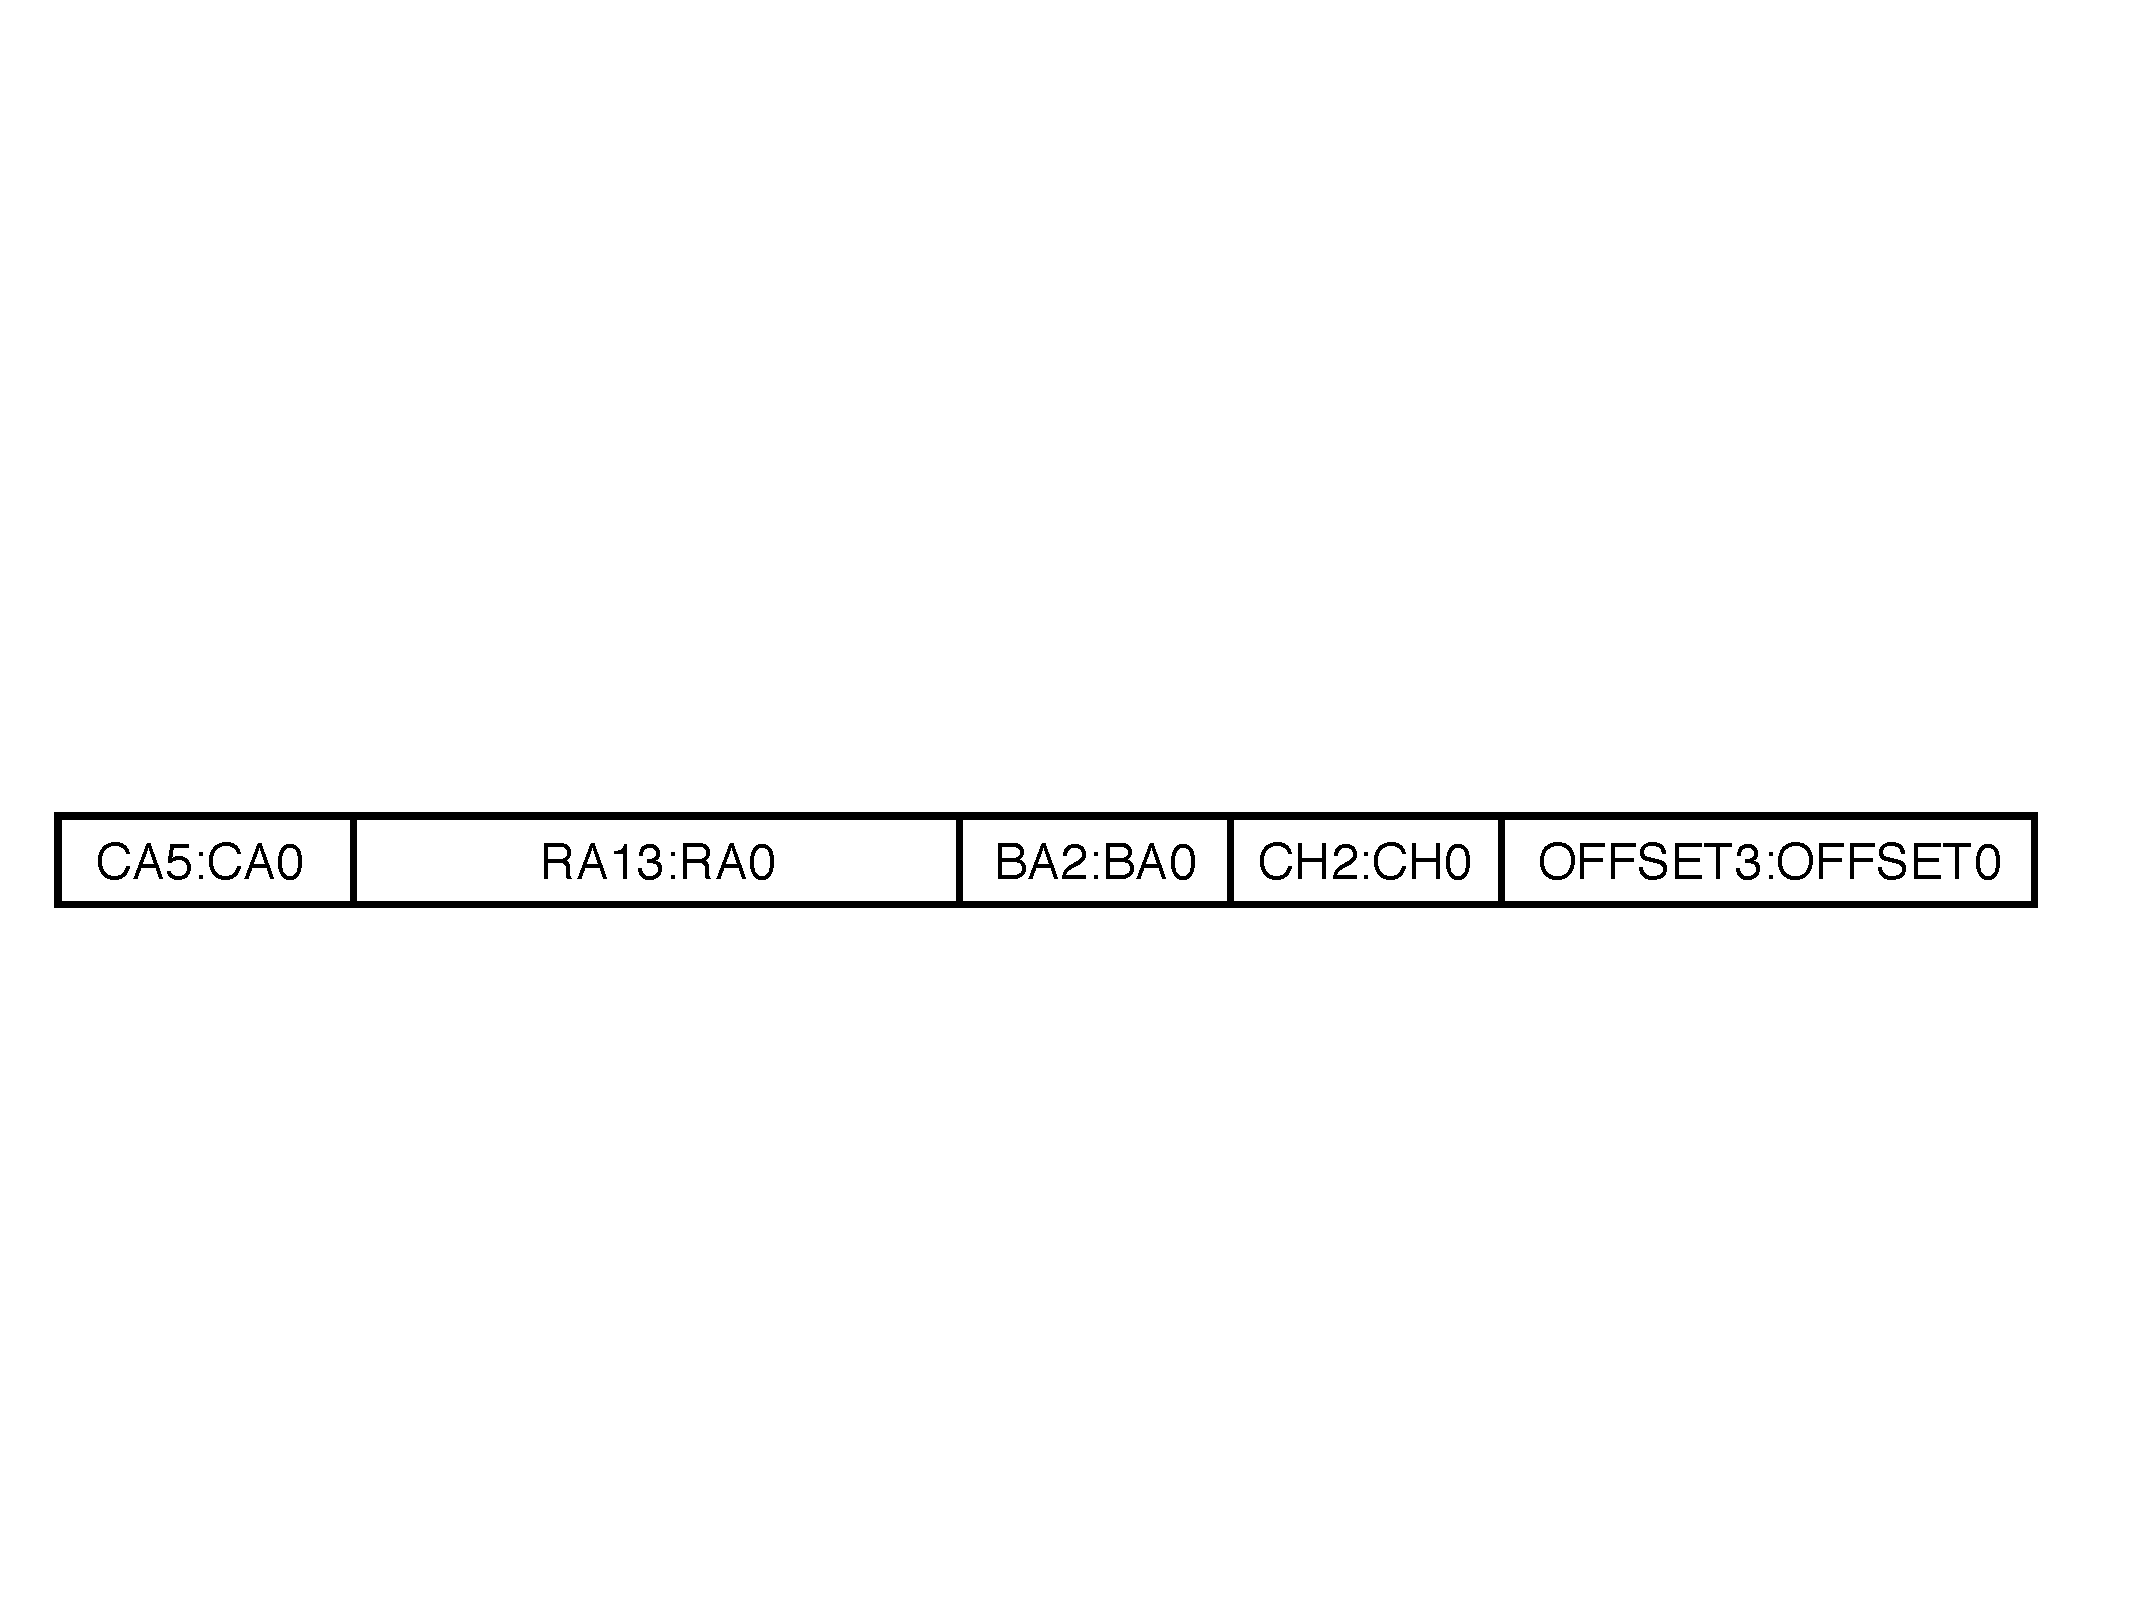
\includegraphics[width=0.98\linewidth]{figures/ChAddressing.pdf} 
\caption{Address mapping for channels.}
\label{fig:mapping}
\end{figure}
%%%%%%%%%%%%%%%%%%%%%%%%%%%%%%%%%%%%%%%%%%%


\begin{figure}[h!] \centering
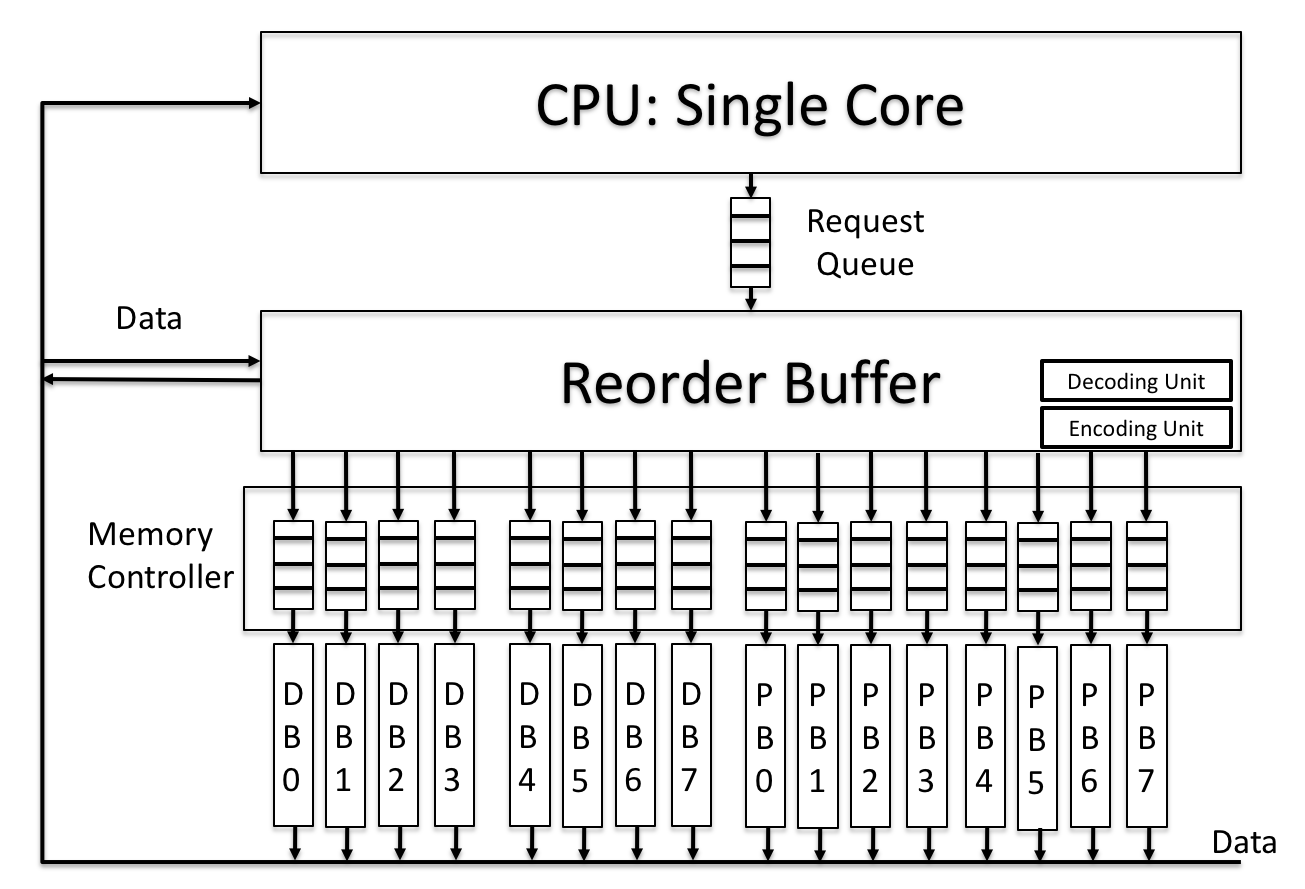
\includegraphics[width=0.9\linewidth]{figures/single-core-cpu.png} 
\caption{Single-core CPU Simulation.}
\label{fig:single-core-cpu}
\end{figure}

\begin{figure}[h!] \centering
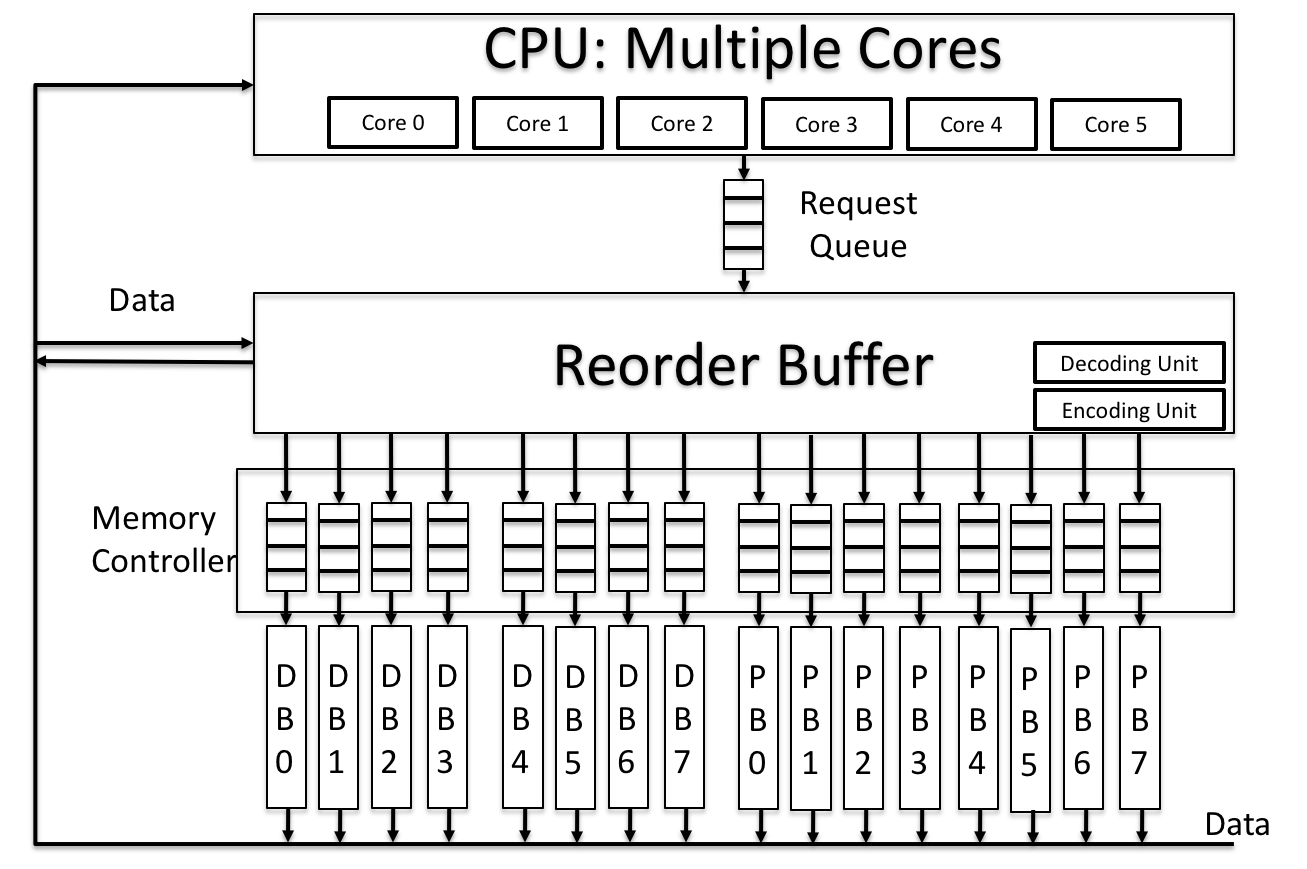
\includegraphics[width=0.9\linewidth]{figures/multi-core-cpu.png} 
\caption{Multi-core CPU Simulation.}
\label{fig:multi-core-cpu}
\end{figure}


%------------------------------------------------------------------------------------
\begin{figure*}[t!] \centering
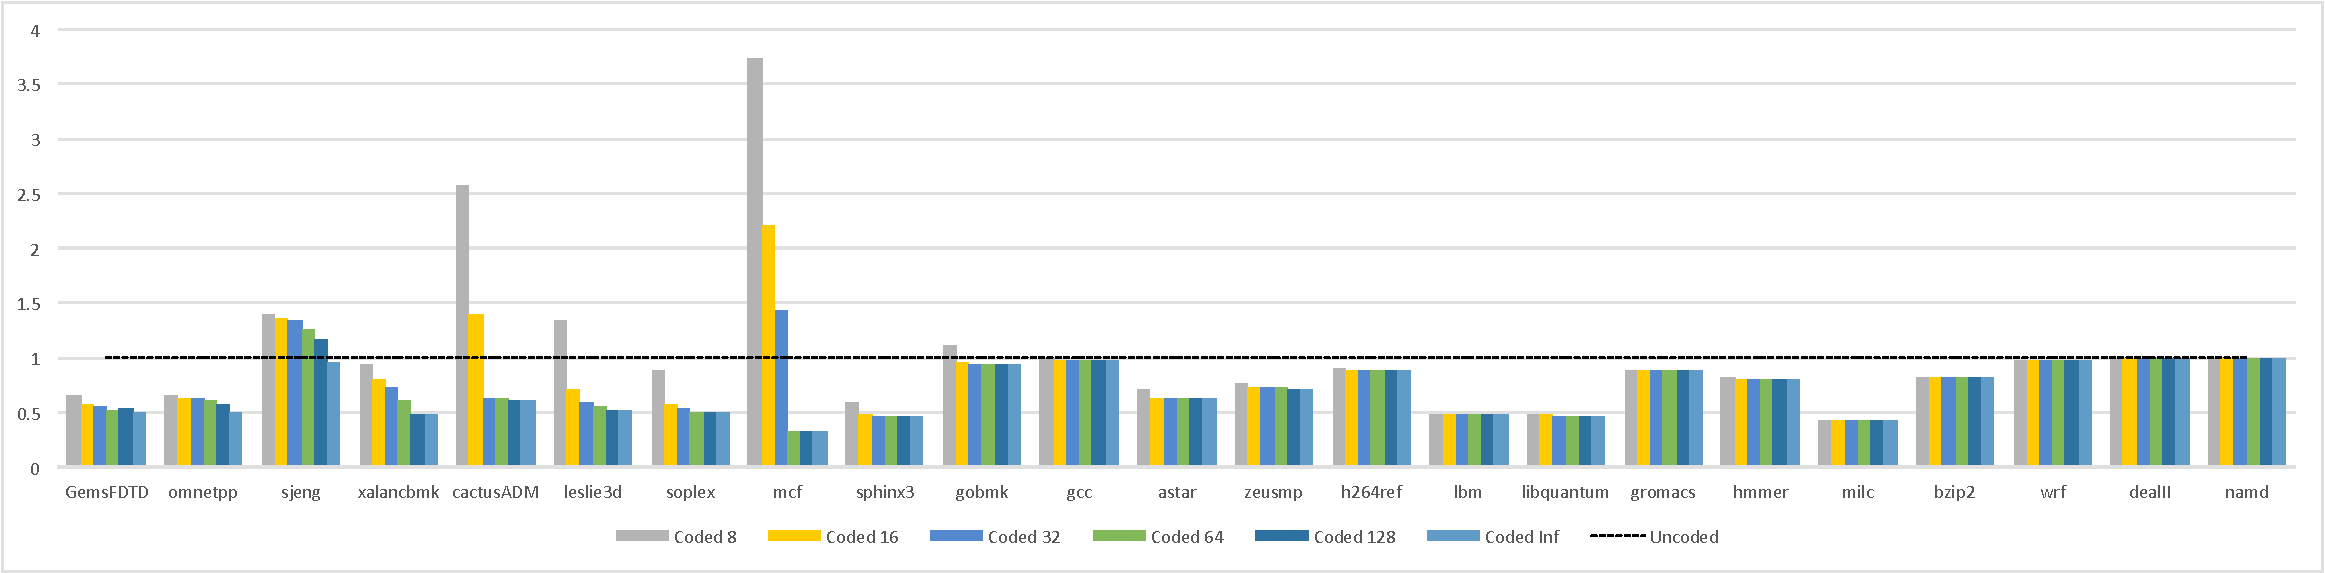
\includegraphics[width=1\linewidth]{figures/spec-cycles-all.pdf} 
\caption{Simulated Number of CPU cycles: Baseline HBM versus Coded HBM across different benchmarks (with reorder buffer size of $\{8,16,32,64,128,\infty\}$). }
\label{fig:spec-cycles}
\end{figure*}
%-----------------------------------------------------------------------------------


\subsection{Methodology}
Our code design was implemented on the Ramulator platform \cite{Ramulator} to evaluate memory access improvements compared to a baseline, uncoded memory layout. This platform allows for excitation of the memory scheduler module with standard benchmarks that represent differentiated and distributed computational and memory access patterns. Experiments were conducted on a single-processor system using the SPEC2006 benchmark \cite{SPEC2006}, and on a $6$-core and $8$-core systems using application traces from an off-the-shelf wireless SoC. 

The single-core architecture for the SPEC2006 benchmark is shown in Figure~\ref{fig:single-core-cpu}, and Figure~\ref{fig:multi-core-cpu} shows the architecture for the $6$-core processor simulation. The instruction traces are mapped to memory requests, which are pushed to a request queue and sent to the memory system's reorder buffer. For each request, the corresponding cycle number, read or write access, and address is stored. After the steps outlined in Section~\ref{sec:reorder}, the bank requests are generated and sent to the HBM memory controller. The corresponding data is sent back to the reorder buffer or to the CPU via the data bus. Since the simulator is cycle accurate, the $6$-core processor simulation may pop multiple requests from the reset queue at the beginning of each cycle.



\subsection{Cycle Simulation Results}
\label{sec:results}


%\subsubsection{Simulation Cycles}
Next, we present the results of SPEC2006 simulation cycles on the proposed coded model and a baseline model. The goal is to simulate the benefits of improved read accesses, which bounds the amount of improvement we can expect in a full hardware implementation. Encoding and decoding can be done offline in parallel and is therefore ignored. We also consider the delays of parity bank writebacks to be negligible. The coded model was evaluated with the following reorder buffer sizes: $\{8,16,32,64,128,\infty\}$.  
%\Ethan{Why are size and depth used interchangeably?}
%The modified model is running multiple times with different reorder buffer size, specifically, the size varies between infinite, 128, 64, 32, 16,8. 
For larger reorder buffer size, the increased memory overhead leads faster accesses.
Thus, the infinite reorder buffer simulation further bounds the performance improvements we expect in practice because no rows are evicted. 
%We can see that the performance improvement is higher when the reorder buffer size is larger. This is the design trade-off between the memory overhead and the performance.

Figure \ref{fig:spec-cycles} compares our memory scheme's performance improvements across different benchmarks. 
For cases such as \texttt{omnetpp} and \texttt{sjeng}, our scheme improves over the uncoded baseline and continues to improve as the buffer size increases.
We also see that for the \texttt{mcf} benchmark, our scheme reduces the read request latency and also reduces the number of CPU cycles to approximately $30\%$ of the uncoded case. This benchmark has the most significant improvements because most of its instructions are memory read requests. 
%Since we don't include the delays of the write back of parity banks and the encoding and the decoding steps, the improvements for each benchmark is the result of the reducing the latency of the read requests with the coded data from parity banks. 
However, \texttt{mcf} hits a performance bottleneck and does not continue improving when the reorder buffer size exceeds 64. This suggests that the \texttt{mcf} memory pattern is clustered such that all the memory requests can be stored in a reorder buffer of this size. The \texttt{mcf} benchmark is made up of a program that implements network simplex code that often works on large chunk of data intermittently~\cite{mcf}. The speed of access (subsequently the speed of the program) in this case improves significantly with the coded memory access.

The \texttt{mlic} benchmark shows reduction to about $40\%$ of the uncoded case for any buffer size. This variety of results suggests that additional improvements can be achieved by combining our scheme with other approaches.



%\Ethan{change to relative improvement like the others?} The number of cycles used for read and write accesses is shown in Figure \ref{fig:spec-cycles1} for the baseline and our coded HBM scheme assuming a reorder buffer of infinite size. This simulation further bounds the performance improvements we expect in practice because no rows are evicted from reorder buffer. For heavy access implementations like MCF, a large improvement can be seen in the reduction of cycles used to serve the requests. \Ethan{add soemthing about omnetpp, soplex, and/or sjeng}
% The subsequent Figures show the performance levels with various reorder buffer size. \par

%
%\begin{figure}[htb] \centering
%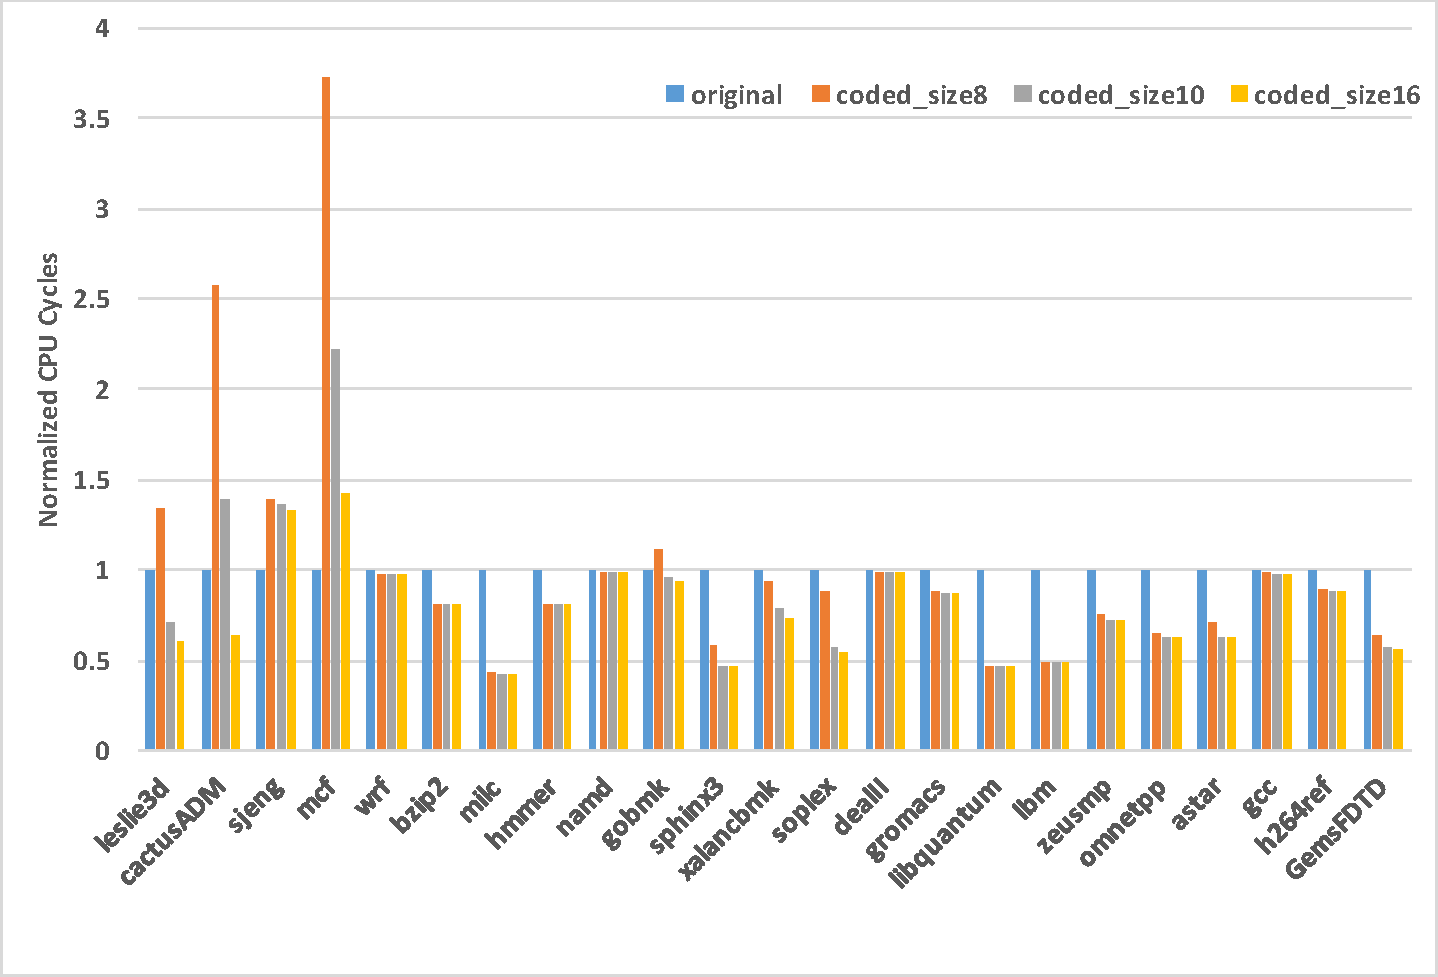
\includegraphics[width=\linewidth]{figures/spec-cycles2.pdf} 
%\caption{Simulated Number of CPU cycles: Baseline HBM versus Coded HBM across different benchmarks (with reorder buffer size of $8, 10, 16$). \Ethan{10 bits or 16 bits? label axes}}
%\label{fig:spec-cycles2}
%\end{figure}
%
%\begin{figure}[htb] \centering
%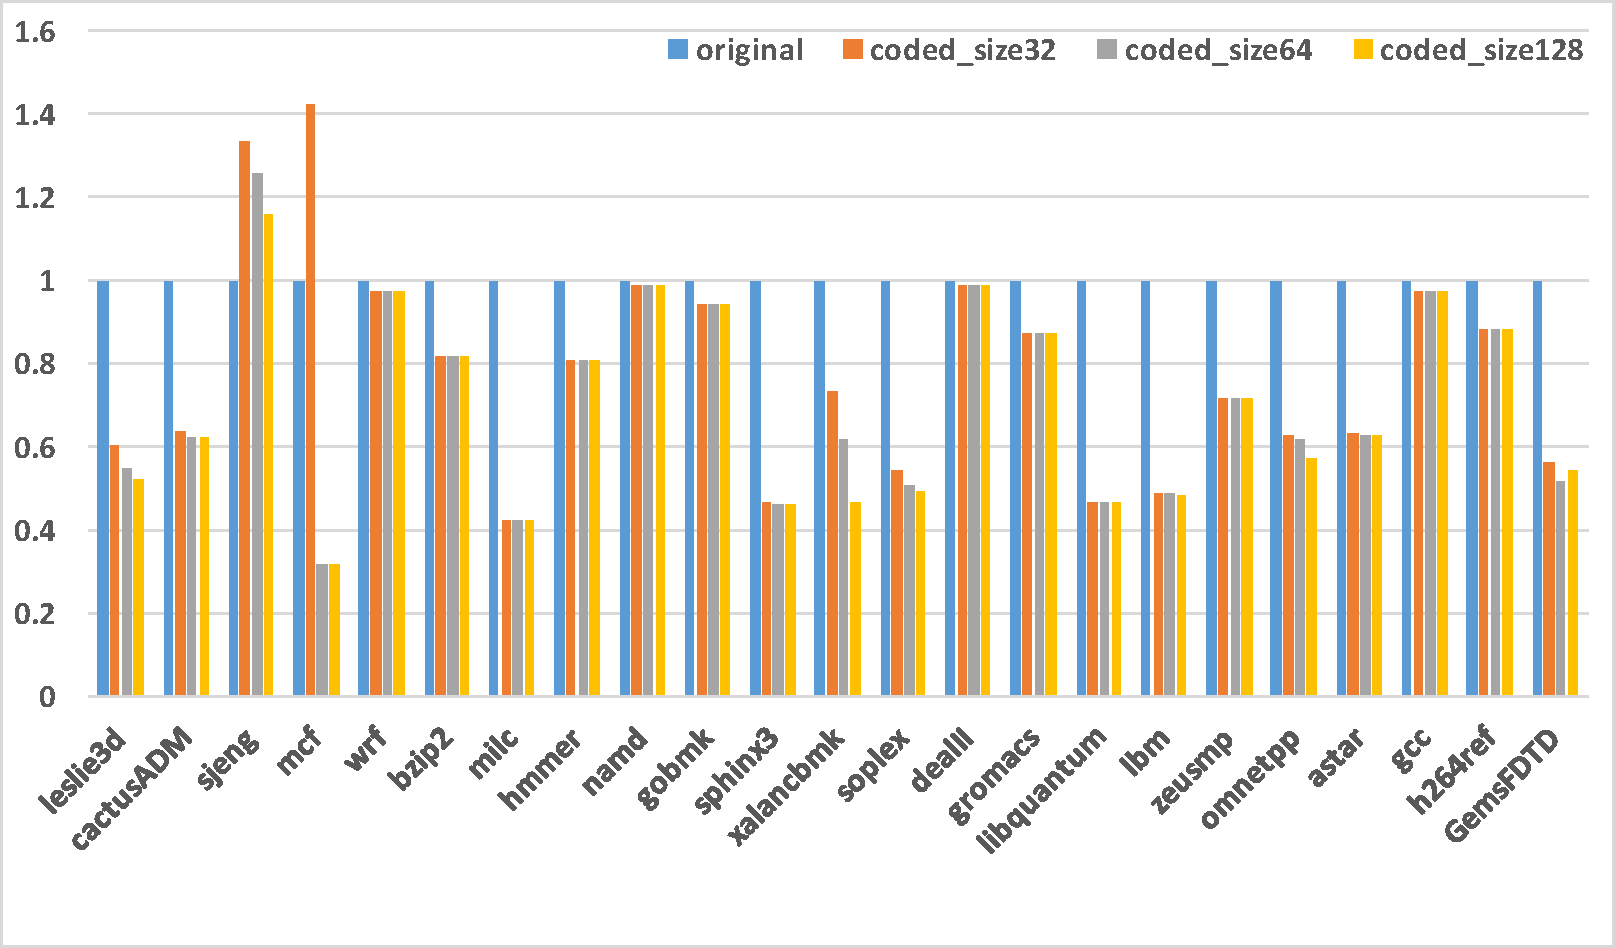
\includegraphics[width=1\linewidth]{figures/spec-cycles3.pdf} 
%\caption{Simulated Number of CPU cycles: Baseline HBM versus Coded HBM across different benchmarks (with reorder buffer size of $32, 64, 128$). \Ethan{label axes}}
%\label{fig:spec-cycles3}
%\end{figure}
%
%\begin{figure}[htb] \centering
%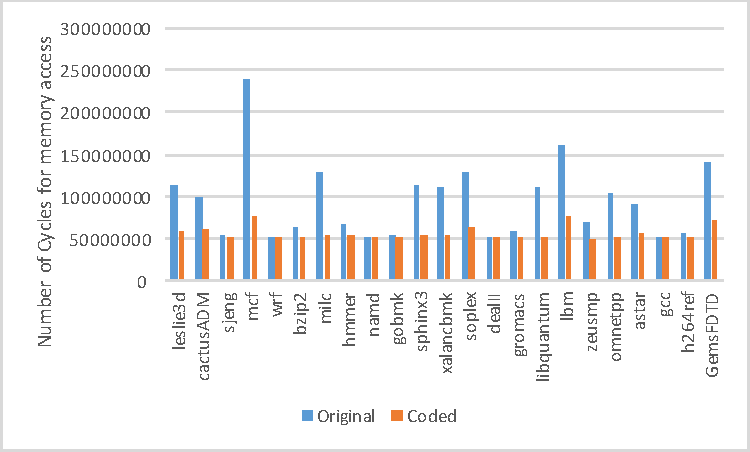
\includegraphics[width=1\linewidth]{figures/spec-cycles1.pdf} 
%\caption{Simulated Number of CPU cycles: Baseline HBM versus Coded HBM across different benchmarks (with infinite reorder buffer size). \Ethan{label axes}}
%\label{fig:spec-cycles1}
%\end{figure}

For the application traces in Figure \ref{fig:lte_umts}, the performance improvements are modest compared to those of the SPEC2006 benchmark. Our scheme hits a performance bottleneck with a reorder buffer size of only $16$ bits. We attribute this to the fact that memory patterns for the application traces are clustered more closely. Again, additional techniques must be used to exceed this observed performance barrier. \\

\begin{figure*}[htb] \centering
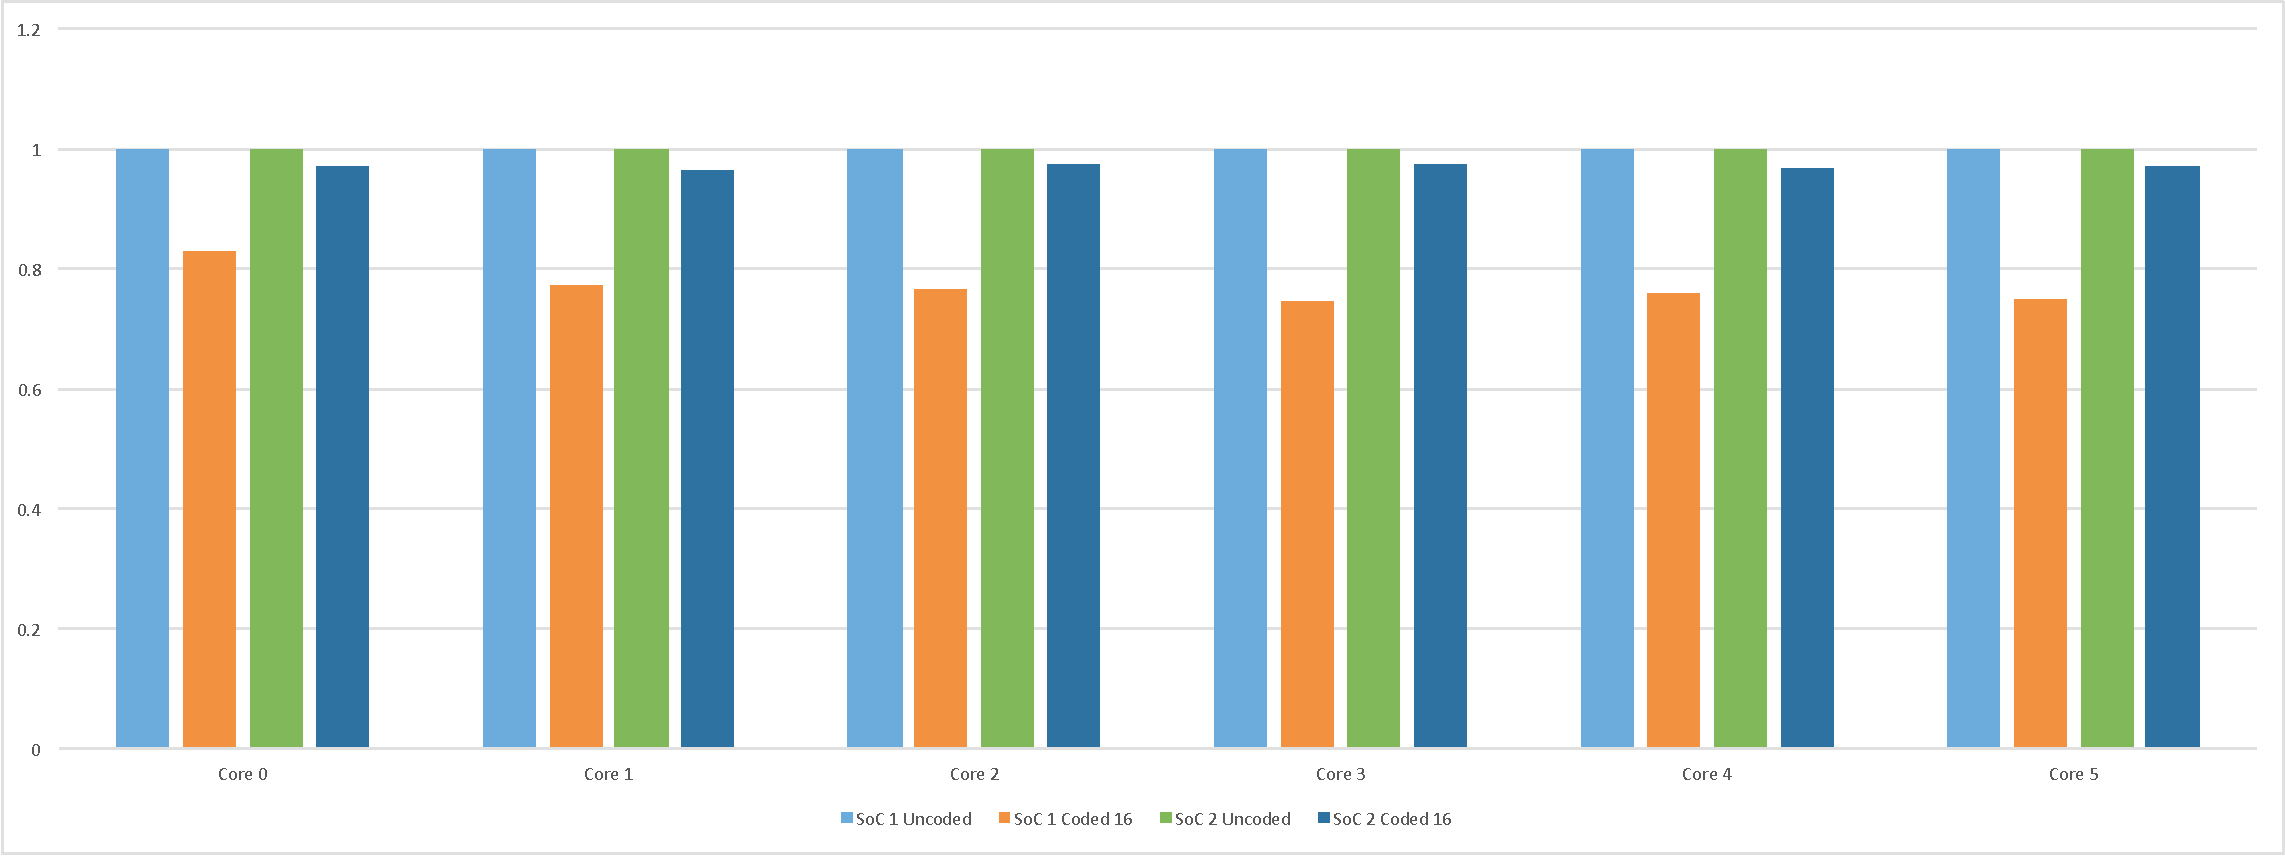
\includegraphics[width=0.75\linewidth]{figures/soc.pdf} 
\caption{Simulated Number of active DRAM cycles: Baseline HBM versus Coded HBM across application-driven wireless SoC traces (reorder buffer size $16$) }
\label{fig:lte_umts}
\end{figure*}

%
%\begin{figure}[htb] \centering
%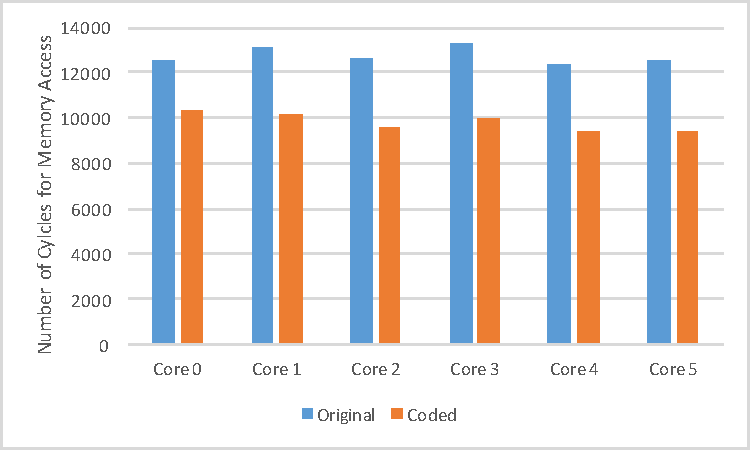
\includegraphics[width=1\linewidth]{figures/lte.pdf} 
%\caption{Simulated Number of active DRAM cycles: Baseline HBM versus Coded HBM across application-driven LTE traces (with reorder buffer size of $16$) }
%\label{fig:lte}
%\end{figure}
%
%\begin{figure}[htb] \centering
%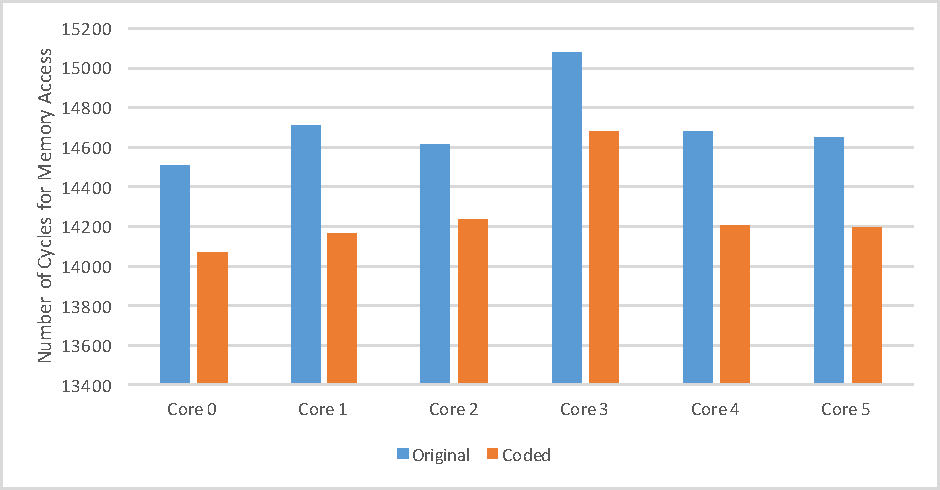
\includegraphics[width=1\linewidth]{figures/umts.pdf} 
%\caption{Simulated Number of active DRAM cycles: Baseline HBM versus Coded HBM across application-driven UTMS traces (with reorder buffer size of $16$) \Ethan{10 bits or 16 bits?}}
%\label{fig:umts}
%\end{figure}


%\subsection{Cost Analysis} 
% Table \ref{tab:size} shows the reorder buffer size as a function of depth. 
% \Ankit{This subsection is just $1$ line?!}\Ethan{Yes, explain figures more}

%\begin{table}
%\begin{tabular}{|l|l|l|l|l|l|}
%\hline \bf Depth & 8 & 16 & 32 & 64 & 128 \\ \hline
%\bf Size & 8KB & 16KB & 32.2KB & 64.5KB & 129KB \\ 
%\hline
%\end{tabular}
%\caption{Reorder Buffer Size under Different Depth}\label{tab:size}
%\end{table}

%%%%%%%%%%%%%%%%%%%%%%%%%%%%%%%%%%%
\begin{figure*}[htb] \centering
%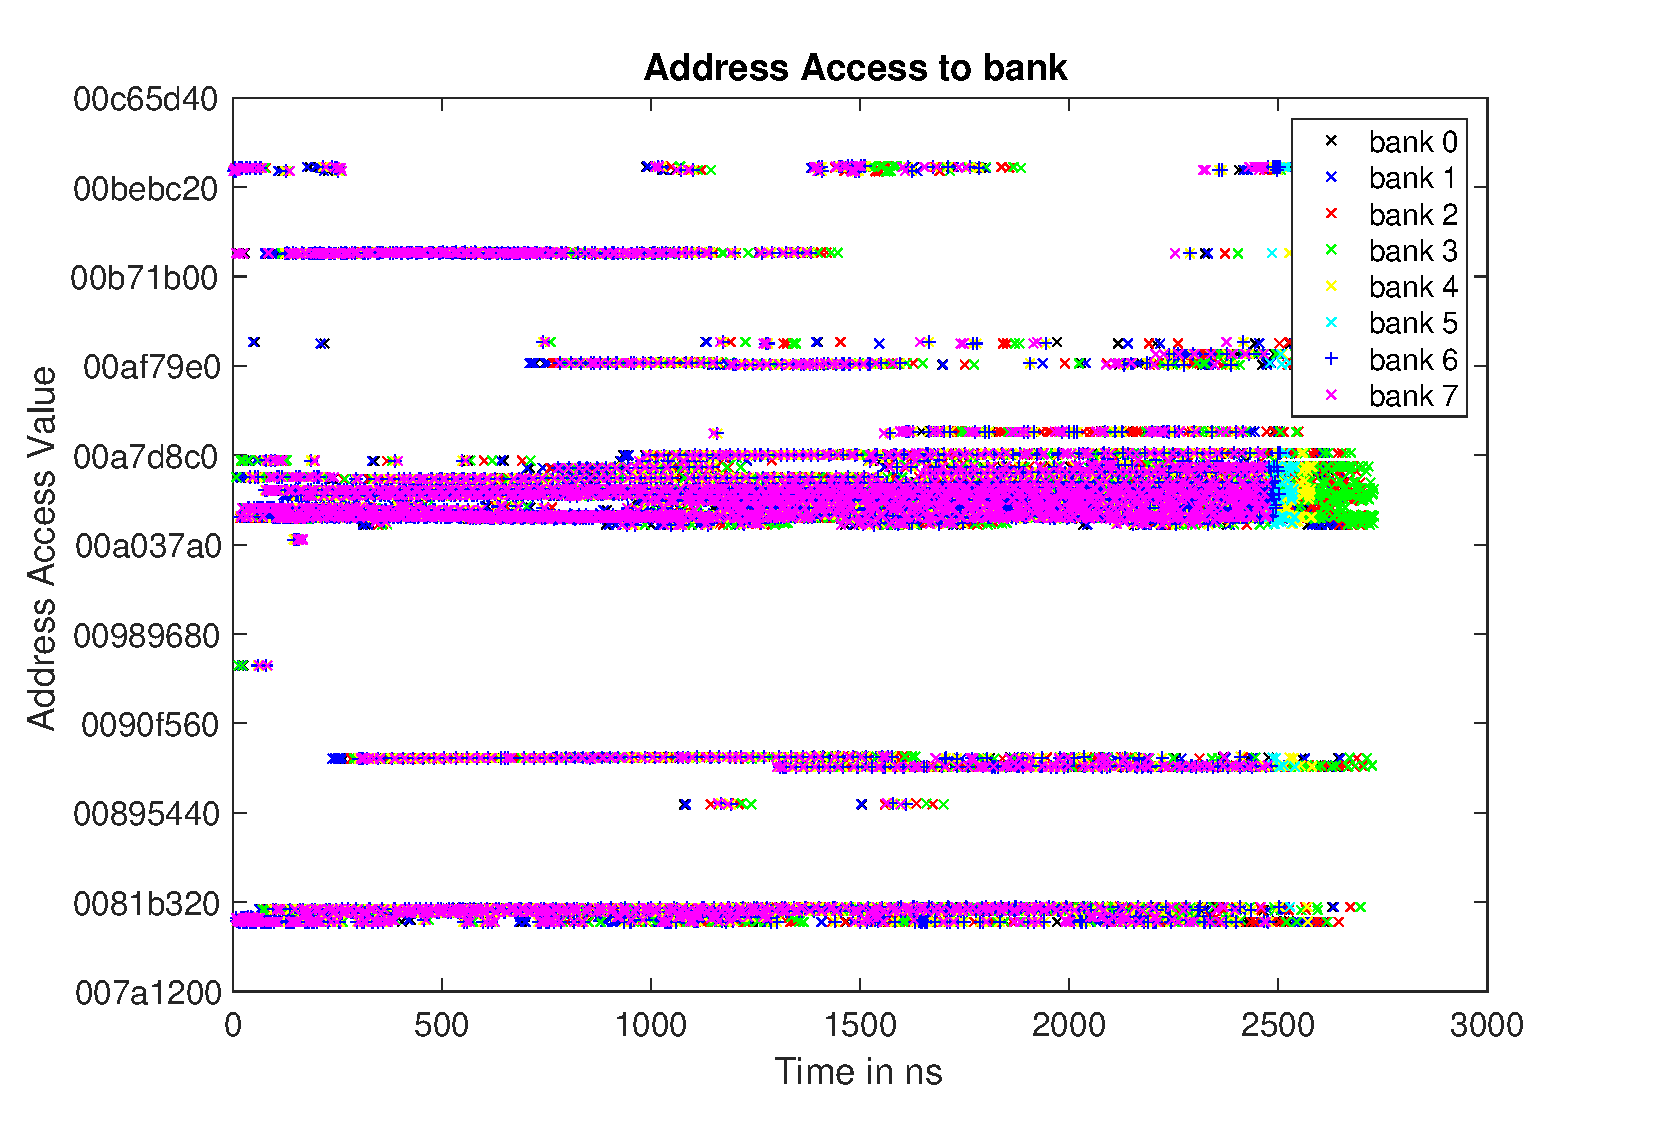
\includegraphics[width=0.50\linewidth]{figures/prefetch1.eps} 
%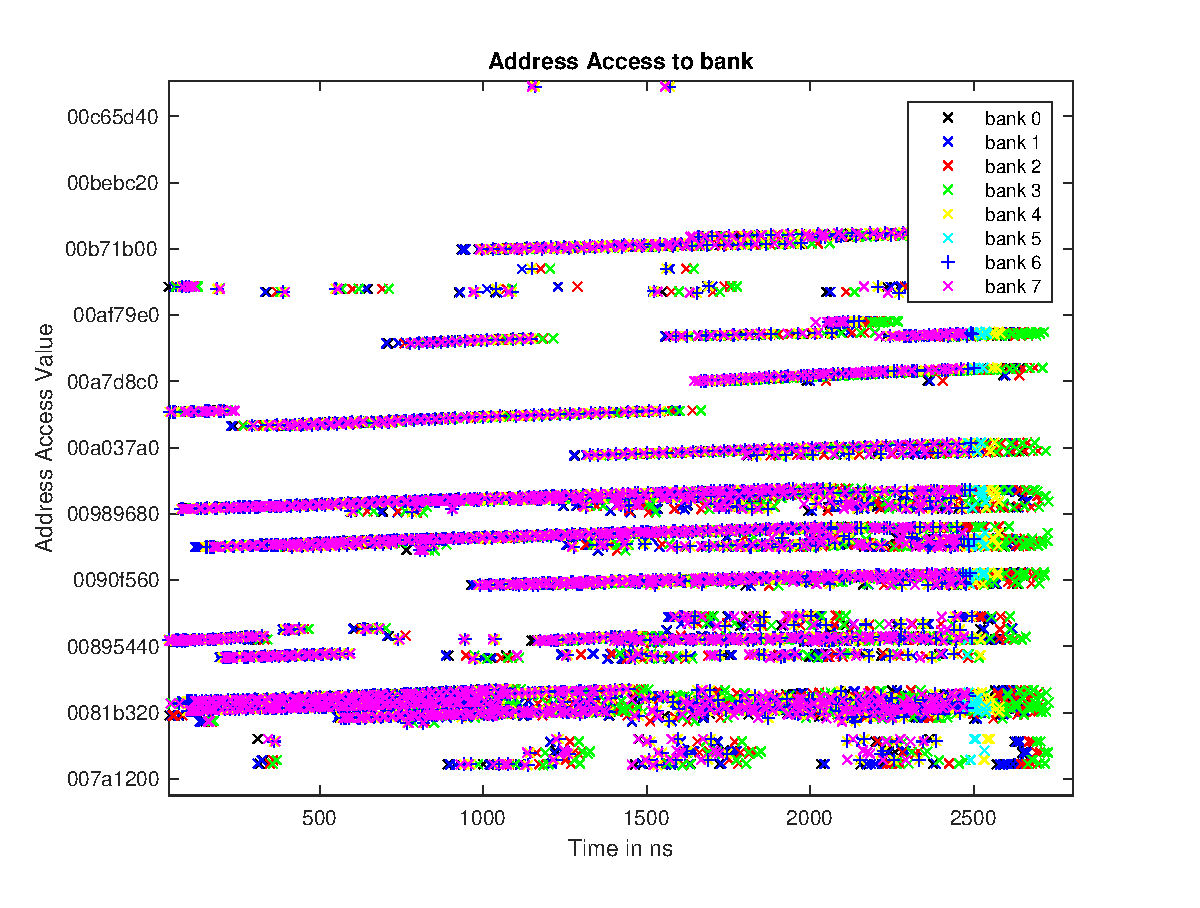
\includegraphics[width=0.46\linewidth]{figures/prefetch2.eps} 
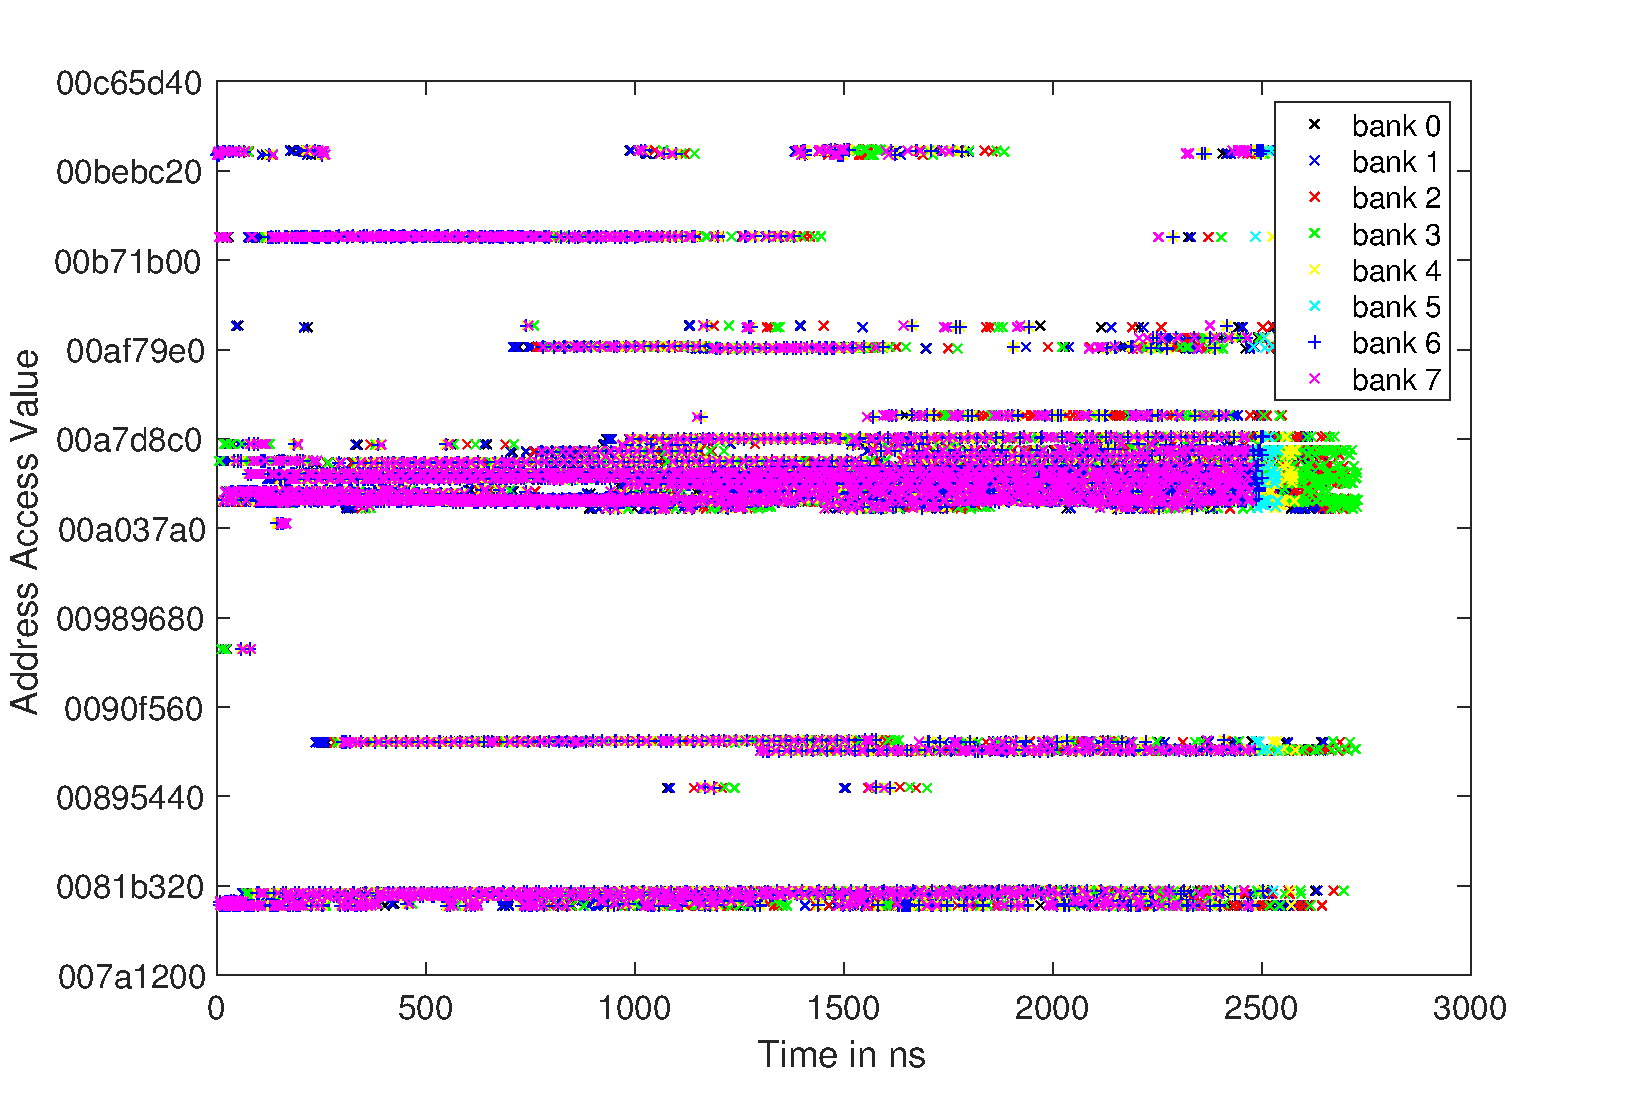
\includegraphics[width=3in,height=0.2\textheight]{figures/prefetch1.pdf}
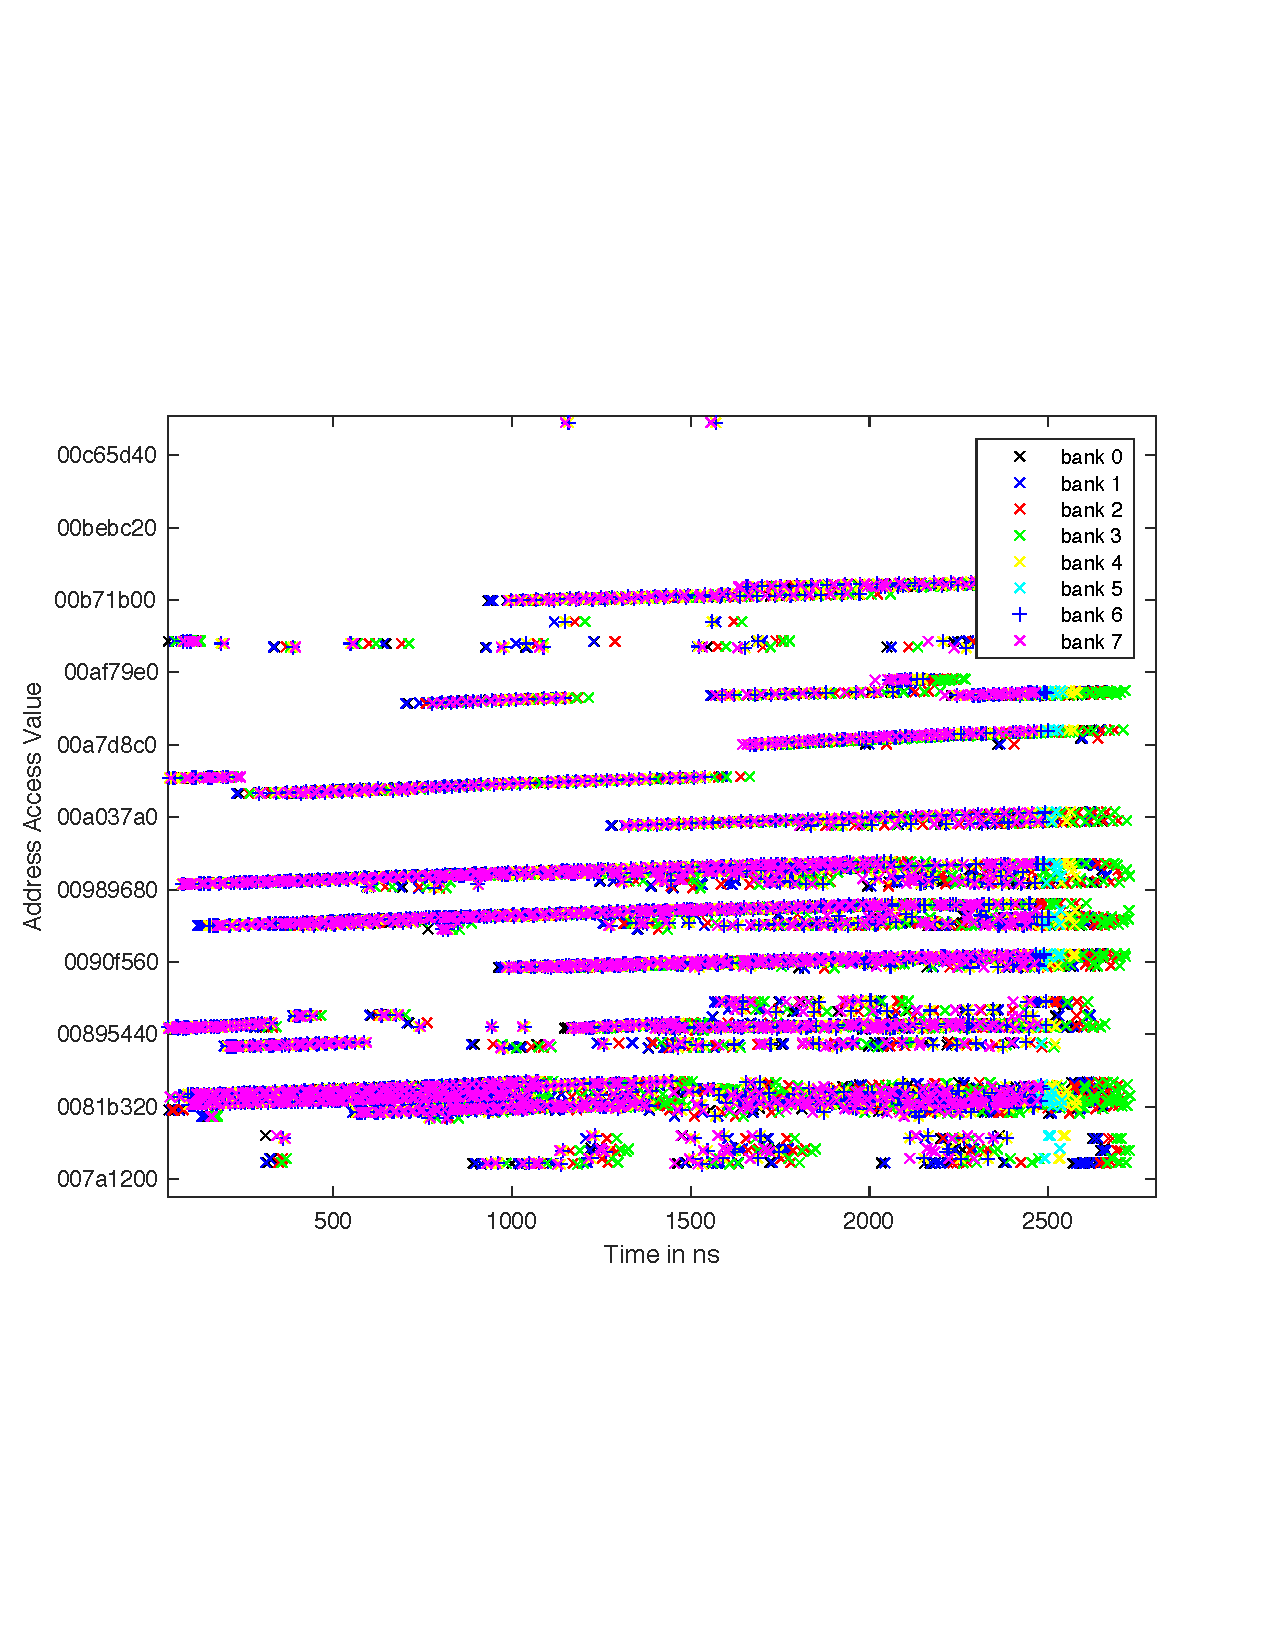
\includegraphics[width=2.6in,height=0.2\textheight]{figures/prefetch2.pdf}
\caption{Memory bank accesses across a 3 $\mu$s trace, which suggest linear access patterns. The right figure is an enlarged version of the top half of the left figure. }
\label{fig:prefetch1}
\end{figure*}
%%%%%%%%%%%%%%%%%%%%%%%%%%%%%%%%%%%

%{\color{blue} \noindent \textbf{Potential improvement using prefetching:}~
%\Ethan{Remove entire subsection?}
%We explore the implementation of a memory prefetching unit, similar to an instruction or cache prefetching unit. This unit can detect linear access patterns to regions in memory.  For example, if a string of memory accesses are issued in sequential byte sized order, then the prefetching unit will predict the next access to be in byte increments. The memory prefetching works by fetching a predicted address from the parity bank during accesses that the parity bank is idle. When future memory accesses are issued, they are first checked with the prefetched data to see if they can be used to decode any subsequent accesses memory accesses. If so, the memory access is obtained from the current accesses and prefetched data. 
%
%For example, say the prefetcher sees 2 consecutive memory requests in a row. It then predicts that the next two accesses, locations $a_0$ and $b_0$, are likely to be accessed in the near future. It reads $a_0 + b_0$ from the parity bank for future use. Next, access to location $a_0$ and $b_0$ are issued to the memory. Now, instead of reading both $a_0$ and $b_0$, only a single location has to be read from in memory, while the other location can be obtained from the prefetched data. This allows for an additional access to be issued from the now free memory bank.  In these cases, it is possible to obtain up to two additional memory accesses in a given cycle, one from the prefetched data and one from the parity bank.
%
%%Implementation of a memory prefetch should only require overhead for space and the associated logic to implement it. Since memory accesses are often stalled due to bank conflicts, checking pending accesses to the prefetched data should require no additional time overhead. As memory accesses wait to be issued in the bank queues, they can simultaneously be checked with the prefetched data. Thus, no extra latency is anticipated by the addition of a memory prefetching unit.
%
%Figure~\ref{fig:prefetch1} shows two plots of memory accesses to a bank with respect to time. The left figure shows the accesses to the memory bank by various cores. The right side figure shows a zoomed view of the accesses in the dense access region. This figure suggests the linearity of accesses. The system can look ahead in the queue to detect the consecutive address request for a memory bank and schedule a prefetch of the associated code.
%
%\noindent {\bf Coding and prefetching:~}One of the ideas explored in this paper is that of proactive prefetching of data from (unused) memory banks to buffers based on the pattern of pending access requests at the memory controller. This creates the opportunities to serve multiple access requests in a given memory cycles and also tries to utilize all the available memory banks throughout the operation of the memory system. Such prefetching based memory designs in the context of {\em uncoded} memory systems has been previously studied in the literature (see e.g.,~\cite{Kim2016, Kadjo2014, Shevgoor2015, JL2013}). To the best of our knowledge, the application of prefetching schemes with coded memory systems has not been explored before.}


%%%%%%%%%%%%%%%%%%%%%%%%%%%%%%%%%%%%%%%%%%%%%%
% Conclusion
%%%%%%%%%%%%%%%%%%%%%%%%%%%%%%%%%
\section{Conclusion}
\label{sec:conclusion}
%\Ethan{Duplicate of abstract?}
This paper proposes a coded memory system that is amenable to multi-bank DRAM architectures such as HBM. Our Reed-Solomon based coding scheme reduces bank conflicts by creating many redundant ways to access a requested data element. This is achieved by assigning some banks to be dedicated parity banks. A memory scheduler then decides which frequently-used data elements should be stored in these parity banks. Simulations on the PARSEC benchmarks show significant reduction in CPU latency when the scheduler's reorder buffer has both finite and infinite size.

%In this paper, we explore the use of coding theory in DDR and high bandwidth memory (HBM) system. Conventional DDR systems use timing optimization techniques around DDR protocol to improve the efficiency of accesses. In this work we propose increasing redundancy to help distribute access across DRAM pages. This will help in efficient retrieval of data. These schemes will be evaluated and optimized with several iterations. The aim is to find the best performing code design scheme given the performance requirement compared to alternatives. Our proposed scheme results in a decrease in the number of contended memory accesses between cores, therefore reducing the overall latency of the system. The reduction in the latency can be seen directly as an increase in the overall system performance. We show that with a memory overhead of  $15$\%, we can enable $4$ extra accesses to a bank while remaining within the given design parameters. We also included emphasis on the code design and optimization of the access scheduler and made significant process in improving the design emulation on the Ramulator platform.
%
%This paper explores the use of coding theory in double data rate (DDR) and high bandwidth memory (HBM) systems. Conventional DDR systems use timing optimization techniques around the DDR protocol to improve access efficiency. This paper proposes utilization of coding techniques to store data across DRAM pages in a redundant manner. The introduced redundancy creates multiple alternatives to access a particular data element stored in the DRAM; consequently making the data retrieval more efficient. This paper proposes a memory design which is based on Reed Solomon codes. The proposed design decreases the number of contended memory accesses between cores. This helps reduce the overall latency of the system, leading to increased performance. Various benchmarking experiments carried out on the proposed design show that the designed memories can enable $4$ extra accesses to a bank while incurring a storage overhead of only $15$\% and remaining within the acceptable values of other design parameters. 

%{\color{blue} \noindent \textbf{Potential improvement using prefetching:}~
%\Ethan{Remove entire subsection?}
%\noindent \textbf{Future Work--Prefetching:}~
\Matt{Is prefetching worth bringing up? Shouldn't this be somewhere before the conclusion?} One potential source of improvement is the addition of a memory prefetching unit, similar to an instruction or cache prefetching unit, which can detect linear access patterns to memory regions. For example, if a sequence of memory accesses is issued in increasing order spaced one byte apart, then a prefetching unit would predict the next access to be one byte past the previous one. 
Prefetching-based memory designs have been studied only in the context of {\em uncoded} memory systems~\cite{Kim2016, Kadjo2014, Shevgoor2015, JL2013}. We can augment our scheme by fetching a predicted address from a parity bank during accesses for which it remains valid but idle. Then for future memory accesses, the controller can check the prefetched data and attempt to complete the request using current accesses and prefetched data. This means that previously occupied banks are available to serve more accesses per cycle. As memory accesses wait to be issued in the bank queues, they can simultaneously be checked with prefetched data. Thus, no extra latency is anticipated by the addition of a memory prefetching unit.
%
Figure~\ref{fig:prefetch1} shows two plots of memory accesses for several banks across time. Both figures suggest linear access patterns and thus larger performance improvements when coding caching is combined with prefetching for this application.

%
%To the best of our knowledge, the application of prefetching schemes with coded memory systems has not been explored before.
%
%For example, say the prefetcher sees 2 consecutive memory requests in a row. It then predicts that the next two accesses, locations $a_0$ and $b_0$, are likely to be accessed in the near future. It reads $a_0 + b_0$ from the parity bank for future use. Next, access to location $a_0$ and $b_0$ are issued to the memory. Now, instead of reading both $a_0$ and $b_0$, only a single location has to be read from in memory, while the other location can be obtained from the prefetched data. This allows for an additional access to be issued from the now free memory bank.  In these cases, it is possible to obtain up to two additional memory accesses in a given cycle, one from the prefetched data and one from the parity bank.
%
%Implementation of a memory prefetch should only require overhead for space and the associated logic to implement it. Since memory accesses are often stalled due to bank conflicts, checking pending accesses to the prefetched data should require no additional time overhead. 
%
%\noindent {\bf Coding and prefetching:~}One of the ideas explored in this paper is that of proactive prefetching of data from (unused) memory banks to buffers based on the pattern of pending access requests at the memory controller. This creates the opportunities to serve multiple access requests in a given memory cycles and also tries to utilize all the available memory banks throughout the operation of the memory system. Such prefetching based memory designs in the context of {\em uncoded} memory systems has been previously studied in the literature (see e.g.,~\cite{Kim2016, Kadjo2014, Shevgoor2015, JL2013}). To the best of our knowledge, the application of prefetching schemes with coded memory systems has not been explored before.


%%%%%%%%%%%%%%%%%%%%%%%%%%%%%%%%%%%%%%%%%%%%%%
% Acknowledgements
%%%%%%%%%%%%%%%%%%%%%%%%%%
% \comment{
% \section{Acknowledgements}
% We would like to thank Dr. Alan Gatherer and Hao Luan from Futurewei Technologies, and Chuiye Kong from The University of Texas at Austin for their guidance and feedback on the work described in this paper. 
% }
%%%%%%% -- PAPER CONTENT ENDS -- %%%%%%%%

\newpage 

%%%%%%%%% -- BIB STYLE AND FILE -- %%%%%%%%
\bibliographystyle{ieeetr}
\bibliography{tex_files/ref}
%%%%%%%%%%%%%%%%%%%%%%%%%%%%%%%%%%%%

\end{document}



%%%%%%%%%%%%%%%%%%%%%%%%%%%%%%%%%%%%%%%%%%%%%%
% Appendices
%%%%%%%%%%%%%%%%%%%%%%%%%%%%%%%%%
%\section{Conclusion}
\label{sec:conclusion}
%\Ethan{Duplicate of abstract?}
This paper proposes a coded memory system that is amenable to multi-bank DRAM architectures such as HBM. Our Reed-Solomon based coding scheme reduces bank conflicts by creating many redundant ways to access a requested data element. This is achieved by assigning some banks to be dedicated parity banks. A memory scheduler then decides which frequently-used data elements should be stored in these parity banks. Simulations on the PARSEC benchmarks show significant reduction in CPU latency when the scheduler's reorder buffer has both finite and infinite size.

%In this paper, we explore the use of coding theory in DDR and high bandwidth memory (HBM) system. Conventional DDR systems use timing optimization techniques around DDR protocol to improve the efficiency of accesses. In this work we propose increasing redundancy to help distribute access across DRAM pages. This will help in efficient retrieval of data. These schemes will be evaluated and optimized with several iterations. The aim is to find the best performing code design scheme given the performance requirement compared to alternatives. Our proposed scheme results in a decrease in the number of contended memory accesses between cores, therefore reducing the overall latency of the system. The reduction in the latency can be seen directly as an increase in the overall system performance. We show that with a memory overhead of  $15$\%, we can enable $4$ extra accesses to a bank while remaining within the given design parameters. We also included emphasis on the code design and optimization of the access scheduler and made significant process in improving the design emulation on the Ramulator platform.
%
%This paper explores the use of coding theory in double data rate (DDR) and high bandwidth memory (HBM) systems. Conventional DDR systems use timing optimization techniques around the DDR protocol to improve access efficiency. This paper proposes utilization of coding techniques to store data across DRAM pages in a redundant manner. The introduced redundancy creates multiple alternatives to access a particular data element stored in the DRAM; consequently making the data retrieval more efficient. This paper proposes a memory design which is based on Reed Solomon codes. The proposed design decreases the number of contended memory accesses between cores. This helps reduce the overall latency of the system, leading to increased performance. Various benchmarking experiments carried out on the proposed design show that the designed memories can enable $4$ extra accesses to a bank while incurring a storage overhead of only $15$\% and remaining within the acceptable values of other design parameters. 

%{\color{blue} \noindent \textbf{Potential improvement using prefetching:}~
%\Ethan{Remove entire subsection?}
%\noindent \textbf{Future Work--Prefetching:}~
\Matt{Is prefetching worth bringing up? Shouldn't this be somewhere before the conclusion?} One potential source of improvement is the addition of a memory prefetching unit, similar to an instruction or cache prefetching unit, which can detect linear access patterns to memory regions. For example, if a sequence of memory accesses is issued in increasing order spaced one byte apart, then a prefetching unit would predict the next access to be one byte past the previous one. 
Prefetching-based memory designs have been studied only in the context of {\em uncoded} memory systems~\cite{Kim2016, Kadjo2014, Shevgoor2015, JL2013}. We can augment our scheme by fetching a predicted address from a parity bank during accesses for which it remains valid but idle. Then for future memory accesses, the controller can check the prefetched data and attempt to complete the request using current accesses and prefetched data. This means that previously occupied banks are available to serve more accesses per cycle. As memory accesses wait to be issued in the bank queues, they can simultaneously be checked with prefetched data. Thus, no extra latency is anticipated by the addition of a memory prefetching unit.
%
Figure~\ref{fig:prefetch1} shows two plots of memory accesses for several banks across time. Both figures suggest linear access patterns and thus larger performance improvements when coding caching is combined with prefetching for this application.

%
%To the best of our knowledge, the application of prefetching schemes with coded memory systems has not been explored before.
%
%For example, say the prefetcher sees 2 consecutive memory requests in a row. It then predicts that the next two accesses, locations $a_0$ and $b_0$, are likely to be accessed in the near future. It reads $a_0 + b_0$ from the parity bank for future use. Next, access to location $a_0$ and $b_0$ are issued to the memory. Now, instead of reading both $a_0$ and $b_0$, only a single location has to be read from in memory, while the other location can be obtained from the prefetched data. This allows for an additional access to be issued from the now free memory bank.  In these cases, it is possible to obtain up to two additional memory accesses in a given cycle, one from the prefetched data and one from the parity bank.
%
%Implementation of a memory prefetch should only require overhead for space and the associated logic to implement it. Since memory accesses are often stalled due to bank conflicts, checking pending accesses to the prefetched data should require no additional time overhead. 
%
%\noindent {\bf Coding and prefetching:~}One of the ideas explored in this paper is that of proactive prefetching of data from (unused) memory banks to buffers based on the pattern of pending access requests at the memory controller. This creates the opportunities to serve multiple access requests in a given memory cycles and also tries to utilize all the available memory banks throughout the operation of the memory system. Such prefetching based memory designs in the context of {\em uncoded} memory systems has been previously studied in the literature (see e.g.,~\cite{Kim2016, Kadjo2014, Shevgoor2015, JL2013}). To the best of our knowledge, the application of prefetching schemes with coded memory systems has not been explored before.

\comment{
\section{HBM details: removed from background sections}

% Each HBM channel is expected to provide a 128-bit data interface that supports up to 1-2 Gbps of data rate per signal equivalent to 500-1000MHz of DDR memory. This is equivalent to 16-32 GB/sec of bandwidth per channel. With 8 channels stacked together it can provide 128-256 GB/sec of access bandwidth per stack. 

% The HBM specification document lists two modes of operation: legacy mode and pseudo channel mode. A memory controller can support either the legacy or the pseudo channel mode. 

% In case of the legacy mode, each read or write transaction transfers 256 bits in a burst that consists of 2 cycles of 128 bits each. In pseudo channel mode, the 128-bit bus is split into 2 individual 64-bit segments. On each segment, a read or write transaction transfers 256 bits as well, but in a burst that lasts 4 cycles (of 64 bits each). The pseudo channel conceptually divides the memory of a single channel in half and assigns each half to a fixed pseudo channel. The pseudo channels share the same address and command bus: you can send a command and addresses to one pseudo channel or the other, but not to both.
% }
